\documentclass[18pt, a4paper]{extarticle}
\usepackage[utf8]{inputenc}
\usepackage[english,russian]{babel}
\usepackage[14pt]{extsizes}
\usepackage[left=5mm, top=5mm, right=5mm, bottom=20mm, nohead, footskip=5mm]{geometry}
\usepackage{indentfirst}
\usepackage{misccorr}
\usepackage{graphicx}
\usepackage{tikz}
\usetikzlibrary{positioning}
\usepackage{amsmath}
\usepackage{amsfonts}
\usepackage{longtable}
\usepackage{amssymb}
\usepackage{multirow}
\usepackage{hhline}
\usepackage{extarrows}
\usepackage{hyperref}
\usepackage{mmap}
\usepackage{wrapfig}

\title{Математическая логика и теория алгоритмов}
\author{Лекции Д.Е. Пальчунова для 1 курса ФИТ НГУ}
\date{2 семестр, 2019 г.}

\newcommand{\opred}[1]{\textbf{\textsc{Определение #1}}}
\newcommand{\predl}[1]{\textbf{\textsc{Предложение #1}}}
\newcommand{\sled}[1]{\textbf{\textsc{Следствие #1}}}
\newcommand{\teor}[1]{\textbf{\textsc{Теорема #1}}}
\newcommand{\zam}[1]{\textbf{\textsc{Замечание #1}}}
\newcommand{\lemma}[1]{\textbf{\textsc{Лемма #1}}}

\newcommand{\opredT}[2]{\textbf{\textsc{Определение #1}(#2).}}
\newcommand{\predlT}[2]{\textbf{\textsc{Предложение #1}(#2).}}
\newcommand{\sledT}[2]{\textbf{\textsc{Следствие #1}(#2).}}
\newcommand{\teorT}[2]{\textbf{\textsc{Теорема #1}(#2).}}

\newcommand{\lot}[3]{#1_#2,\dots,#1_#3}

\newcommand{\anonsection}[1]{\section*{\S #1}\addcontentsline{toc}{subsection}{\S #1}}
\newcommand{\ampersand}{\;\&\;}
\newcommand{\Gm}{\Gamma}
\newcommand{\vp}{\varphi}
\newcommand{\vd}{\vdash}
\newcommand{\vD}{\vDash}
\newcommand{\al}{\alpha}
\newcommand{\sg}{\sigma}
\newcommand{\ovl}[1]{\overline{#1}}
\newcommand{\centr}[1]{\makebox[\linewidth]{#1}}
\newcommand{\primer}{\textbf{Пример:\;}}
\newcommand{\rightdok}{\boxed{(\Rightarrow)}}
\newcommand{\leftdok}{\boxed{(\Leftarrow)}}
\newcommand{\mA}{\mathfrak{A}}
\newcommand{\mB}{\mathfrak{B}}
\newcommand{\mC}{\mathfrak{C}}
\newcommand{\mJ}{\mathfrak{J}}
\newcommand{\mL}{\mathfrak{L}}
\newcommand{\mR}{\mathfrak{N}}
\newcommand{\mM}{\mathfrak{M}}
\newcommand{\dok}{\textsc{Доказательство:}}
\newcommand{\dokup}{\textsc{Доказательство: упражнение.}}
\newcommand{\bezdok}{\textsc{Без доказательства.}}
\DeclareUnicodeCharacter{22AD}{\nvDash}
\DeclareUnicodeCharacter{22AC}{\nvdash}

\definecolor{linkc}{rgb}{0.33,	0.51,	0.78}

\hypersetup{
    colorlinks=true,
    urlcolor=linkc,
    linkcolor=black,
    linkbordercolor=red,
    pdfborderstyle={/S/U/W 1}
    pdfpagemode=FullScreen,
    }

\begin{document}
\linespread{1.3}
 \fontsize{19pt}{22pt}\selectfont
\maketitle

\tableofcontents
\leavevmode\begin{center}
    Если нашли очепятки, то пишите \href{https://vk.com/id177003653}{\underline{мне}}, я поправлю :)
\end{center}

\newpage
\anonsection{10. Секвенциальное исчисление высказываний}

В начале курса мы изучали логику высказываний. Высказывание - это повествовательное предложение о состоянии мира, которое может быть истинным или ложным. Например, высказывание "\textit{Число 2 - это простое число}"{} является истинным, а высказывание "\textit{В неделе 5 дней}"{} ложным. Чтобы понять секвенции, мы определим следующие вещи.\\

\textbf{\textsc{Определение 10.1.}} 

Пусть $\Gamma = \langle\varphi_1,\ldots,\varphi_n\rangle$ - конечная последовательность формул.

Тогда \textbf{cеквенциями} называются выражения вида:

\qquad 1) \;\;$\Gamma \vdash \varphi$ \;\;(из $\Gamma$ выводимо $\varphi$)

\qquad 2) \;\;$\vdash \varphi$ \;\;($\varphi$ выводится)

\qquad 3) \;\;$\Gamma \vdash$ \;\;($\Gamma$ противоречиво)

\textbf{Аксиома:} $\varphi \vdash \varphi$.\\

\textbf{Правила вывода:}\\

\begin{tabular}{ll}
    1) $\displaystyle \frac{\Gamma \vdash \varphi; \; \Gamma \vdash \psi}{\Gamma \vdash (\varphi \ampersand \psi)}$ & \qquad
    2) $\displaystyle \frac{\Gm \vdash (\varphi \ampersand \psi)}{\Gm \vdash \varphi}$
    \\\\
    3) $\displaystyle \frac{\Gm \vdash (\varphi \ampersand \psi)}{\Gm \vdash \psi}$ & \qquad
    4) $\displaystyle \frac{\Gm \vdash \varphi}{\Gm \vdash (\varphi\vee\psi)}$
    \\\\
    5) $\displaystyle \frac{\Gm \vdash \psi}{\Gm \vdash (\varphi\vee\psi)}$ & \qquad
    6) $\displaystyle \frac{\Gm,\varphi \vdash \xi; \; \Gm,\psi \vdash \xi; \; \Gm \vdash (\varphi \vee \psi)}{\Gm \vdash \xi}$
    \\\\
    7) $\displaystyle \frac{\Gm,\varphi \vdash \psi}{\Gm\vdash (\varphi\to\psi)}$ & \qquad
    8) $\displaystyle \frac{\Gm\vdash\varphi;\;\Gm\vdash(\varphi\to\psi)} {\Gm\vdash\psi}$ (modus ponens)
\end{tabular}

\begin{tabular}{ll}
    9) $\displaystyle \frac{\Gm,\lnot \varphi \vdash}{\Gm\vdash\varphi}$ & \qquad
    10) $\displaystyle \frac{\Gm\vdash\lnot\varphi;\;\Gm\vdash\varphi}{\Gm\vdash}$
    \\\\
    11) $\displaystyle \frac{\Gm,\varphi,\psi,\Gm_1 \vdash \xi}{\Gm,\psi,\varphi,\Gm_1 \vdash \xi}$ & \qquad
    12) $\displaystyle \frac{\Gm\vdash\varphi}{\Gm,\psi\vdash\varphi}$
\end{tabular}\leavevmode\\

Секвенциальное исчисление высказываний (ИВ) - это, в некотором смысле, попытка смоделировать логическое мышление человека, попытка описать некоторые простейшие способы рассуждений, которые позволяют переходить от одних истинных утверждений к другим истинным утверждениям, т.е. переходить от одних секвенций к другим секвенциям с помощью правил вывода, сохраняя логичное следование высказываний.

Знак $\vd$ обозначает логическое следование. Запись вида $\lot \vp 1 n\vd\psi$ читается, как "\textit{из формул $\lot \vp 1 n$ (логически) следует формула $\psi$}"{}. Запись вида $\lot \vp 1 n\vd$ читается, как "\textit{формулы $\lot \vp 1 n$ противоречивы}"{}. Запись вида $\vd\psi$ читается, как "\textit{формула $\psi$ доказуема}"{}.\\

\textbf{\textsc{Определение 10.2.}} 

Последовательность секвенций $S_1,\ldots,S_n$ называется \textbf{доказательством}, если каждая секвенция $S_i$ -  это либо аксиома, либо получена из предыдущих однократным применением некоторого правила вывода.

Секвенция $S$ называется \textbf{доказуемой}, если $\exists$ доказательство $S_1,\ldots,S_n$, заканчивающееся на $S$, т.е. $S_n = S$.\\

\textbf{\textsc{Лемма 10.3.}}

a) Если последовательность $S_1,\ldots S_n$ -  доказательство, где $k\leqslant n$, то\\ $S_1,\ldots,S_k$ -  доказательство:

б) $S_1,\ldots S_n$ -  доказательство, где $k\leqslant n \Rightarrow S_k$ -  доказуема.\\

\textbf{\textsc{Определение 10.4.}}

Дадим определение \textbf{дерева секвенций}:

1) Каждая секвенция $S$ -  дерево;

2) Если $D_1,\ldots D_k$ -  деревья секвенций, $S$ -  секвенция, то такая 

конструкция: $\displaystyle \frac{D_1;\ldots;D_k}{S}$ -  дерево секвенций;

3) Других деревьев секвенций нет.\\

Данные деревья секвенций - как раз те самые логические цепи, где мы от одного суждения переходим к другому, не теряя логичность рассуждения. Все деревья начинаются с одной единственной аксиомы $\vp\vd\vp$, где мы подставляем за место $\vp$ нашу формулу. Далее к аксиоме, что мы установили, применяем правило вывода, делая \textit{новый уровень} дерева. В дальнейшем работа с секвенциями будет проходить именно с помощью деревьев. Чуть позже мы рассмотрим примеры таких деревьев.\\

\textbf{\textsc{Определение 10.5.}}

Для удобства в будущих доказательствах мы введём следующие определения:

а) $V(D)$ -  множество \textbf{вершин} дерева $D$.

\qquad 1) Если $D = S$, то $V(D) = S$.

\qquad 2) Если $D = \displaystyle \frac{D_1;\ldots;D_k}{S}$, то $V(D) = V(D_1)\cup\ldots\cup V(D_k)$.

б) $p(D)$ -  \textbf{переходы.}

\qquad 1) Если $D = S$, то $p(D) = \varnothing$.

\qquad 2) Если $D = \displaystyle \frac{D_1;\ldots;D_k}{S}$, то $p(D) = p(D_1)\cup\ldots\cup p(D_k) \cup \displaystyle \Big\{ \frac{S_1;\ldots;S_k}{S}\Big\}$,

\qquad где $D_i = \displaystyle\frac{\cap}{S_i}$.

Здесь $\cap$ - верхняя часть дерева. Ещё $\cap$ иногда обозначают просто многоточием.

в) $h(D)$ -  \textbf{высота} дерева.

\qquad 1) Если $D = S$, то $h(D) = 1$.

\qquad 2) Если $D = \displaystyle \frac{D_1;\ldots;D_k}{S}$, то $h(D) = \max (h(D_1),\ldots h(D_k)) + 1$.\\

\textbf{\textsc{Определение 10.6.}} 

Дерево секвенций называется \textbf{деревом вывода}, если все его вершины являются аксиомами, а все переходы являются частными случаями правил вывода.\\

\textbf{\textsc{Предложение 10.7.}} 

Секвенция $S$ является доказуемой $\Leftrightarrow \exists$ дерево вывода $D = \displaystyle\frac{\cap}{S}$, заканчивающееся на эту секвенцию. \\

\textsc{Доказательство:} 

$\boxed{(\Rightarrow)}$ Пусть $S$ - доказуема, тогда $\exists S_1,\ldots,S_n = S$ - доказательство. Далее по индукции:

1) \underline{$n = 1$}: $S_1 = S$ ($S$ -  аксиома). $D = S$ -  дерево вывода.

2) \underline{$<n\to n$} (индукция по построению):

Есть $S_{i_1},\ldots,S_{i_m}; \; i_1,\ldots,i_m < n;$ $\displaystyle \frac{S_{i_1};\ldots;S_{i_m}}{S}, \; m = $1, 2 или 3.

Если $S_1,\ldots,S_{i_k}$ -  доказательство, $k\leqslant m, \; i_k < n \Rightarrow$ (по индукционному предположению) $\exists D_{i_k} = \displaystyle \frac{\cap}{S_{i_k}}$ -  дерево вывода.\\

$\displaystyle \frac{D_{i_1};\ldots; D_{i_m}}{S} = \frac{\displaystyle \frac{\cap}{S_{i_1}};\ldots;\frac{\cap}{S_{i_m}}}{S}$ -  дерево вывода (\textit{упражнение}).\\

$\boxed{(\Leftarrow)}$ Пусть $D = \displaystyle \frac{\cap}{S}$ -  дерево вывода. Обозначим $n = h(D)$. Далее по индукции:

1) $\underline{n = 1}$: $D = S$ -  аксиома $\Rightarrow$ $S$ -  доказательство.

2) $\underline{<n\to n}$: $D = \displaystyle\frac{D_1;\ldots;D_m}{S}$, где $D_k = \displaystyle\frac{\cap}{S_k}$, откуда $\displaystyle \frac{S_1;\ldots;S_m}{S}$ -  правило вывода.

Тогда $D = \displaystyle\frac{\displaystyle\frac{\cap}{S_1};\ldots;\frac{\cap}{S_m}}{S}$, где $m\leqslant 3$, поскольку у нас нет правил вывода, где есть более трёх поддеревьев наверху.

Поскольку $h(D_k)<n \Rightarrow \exists$ последовательность $S^k_1,\ldots,S^k_{i_k} = S_k$ - доказательство. Откуда $S^1_1,\ldots,S^1_{i_1},\ldots,S_1^m,\ldots,S^m_{i_m}, S$ -  доказательство (\textit{упражнение}).

Предложение доказано.\\

\textbf{\textsc{Определение 10.8.}} 

Дерево секвенций $\displaystyle \frac{S_1;\dots;S_n}{S}\;$ высоты 2 называется \textbf{производным правилом вывода}, если $\exists D =\;\displaystyle \frac{\cap}{S}$, у которого все переходы являются правилами вывода, а вершины - либо аксиомы, либо секвенции $S_1,\dots,S_n$.

Дерево секвенций высоты 2 называется \textbf{допустимым правилом вывода}, если при его добавлении в качестве нового правила вывода множество доказуемых секвенций \underline{не увеличивается}.\\

\textbf{\textsc{Замечание 10.9.}} 

Любое производное правило вывода является \textbf{допустимым}.

\textsc{Доказательство: упражнение.} \\

Важно отметить, что \underline{не любое допустимое правило вывода будет произво}-\underline{дным}.\\\\

\textbf{\textsc{Замечание 10.10.}} 

Следующие правила вывода являются допустимыми:\\

\begin{tabular}{l}
а) $\displaystyle \frac{\psi_1,\dots,\psi_n \vdash \varphi}{\xi_1,\dots,\xi_k \vdash \varphi},\;\{\psi_1,\dots,\psi_n\} \subseteq \{\xi_1,\dots,\xi_k\}$\\\\

б) $\displaystyle \frac{\psi_1,\dots,\psi_n \vdash }{\xi_1,\dots,\xi_k \vdash},\;\{\psi_1,\dots,\psi_n\} \subseteq \{\xi_1,\dots,\xi_k\}$
\end{tabular}\leavevmode\\\\

\begin{tabular}{lll}
в) $\displaystyle \frac{\Gamma \vdash \varphi;\;\Gamma, \varphi \vdash \psi }{\Gamma \vdash \psi}$ \qquad& e) $\displaystyle \frac{\Gamma \vdash}{\Gamma \vdash \varphi}$ \qquad & и) $\displaystyle \frac{\Gamma, \varphi\vdash\psi}{\Gamma,\lnot\psi\vdash\lnot\varphi}$\\\\

г) $\displaystyle \frac{\Gamma_1,\;\varphi,\;\psi,\;\Gamma_2 \vdash \xi}{\Gamma_1, (\varphi\ampersand\psi), \Gamma_2 \vdash \xi}$ \qquad & ж) $\displaystyle \frac{\Gamma,\;\varphi\vdash}{\Gamma\vdash\lnot\varphi}$ \qquad & к) $\displaystyle \frac{\Gamma,\lnot\varphi\vdash\lnot\psi}{\Gamma,\psi\vdash\varphi}$\\\\

д) $\displaystyle \frac{\Gamma \vdash (\varphi\ampersand\lnot\varphi)}{\Gamma\vdash}$ \qquad & з) $\displaystyle \frac{\Gamma\vdash\varphi}{\Gamma,\lnot\varphi\vdash}$ & л) $\displaystyle \frac{\varphi\vdash\psi;\;\psi\vdash\xi}{\varphi\vdash\xi}$\\\\
\end{tabular}\leavevmode\\

\textbf{\textsc{Определение 10.11.}(Семантика исчисления секвенций)}

а) Секвенция $\varphi_1,\dots,\varphi_n\vdash\psi$ называется истинной при данных значениях пропозициональных переменных, если либо $\exists i\leqslant n: \varphi_i\; -\;$ ложная, либо
$\psi\;-\;$ истинная;

б) $\vdash\psi$ истинная, если $\psi\;-\;$ истинная при данных значениях пропозициональных переменных;

в) $\varphi_1,\dots,\varphi_n\vdash$ истинная, если $\exists i\leqslant n: \varphi_i\;-\;$ ложна;

г) $S$ тождественно истинная, если она является истинной при любых входящих в неё значениях пропозициональных переменных.
\newpage

\textbf{\textsc{Теорема 10.12.}(о корректности исчисления секвенций)}

Если секвенция доказуема, то она тождественно истинна.

\textsc{Доказательство:}

Пусть $S\;-\;$ доказуема, тогда $\exists S_1,\dots,S_n\;=\;S\;-\;$ доказательство.

1) $\underline{n=1}$, тогда $S$ -  аксиома, $S=(\varphi\vdash\varphi)$;

2) $\underline{<n\Rightarrow n}.\;\;S_1,\dots, S_n=S$ -  доказательство, $\displaystyle \frac{S_{i_1};\dots;S_{i_m}}{S}\;-\;$ правило вывода.

Очевидно, $i_k < n$. Тогда $S_1,\dots,S_{i_k}$ -  доказательство $\Rightarrow\newline\Rightarrow S_{i_k}$ -  доказуема $\Rightarrow\;$ $S_{i_k}$ -  т.и.

Тогда $\displaystyle \frac{S_{i_1};\dots;S_{i_m}}{S}$ - правило вывода $\Rightarrow S$ - т.и. (\textit{упражнение}).

Теорема доказана.\\

\textbf{\textsc{Определение 10.13.}} 

Пусть $\rho: F \to F,\;F$ -  множество всех формул. Это отображение называется \textbf{подстановкой}, если оно перестановочно с логическими связками.

1) $\rho(\varphi\vee\psi)=(\rho(\varphi)\vee\rho(\psi));$

2) $\rho(\varphi\ampersand\psi)=(\rho(\varphi)\ampersand\rho(\psi));$

3) $\rho(\varphi\to\psi)=(\rho(\varphi)\to\rho(\psi));$

4) $\rho(\lnot\varphi)=\lnot\rho(\varphi)$.\\

\textbf{\textsc{Теорема 10.14.}(о подстановке)} 

Каждая подстановка сохраняет доказуемость секвенций, то есть если \\$\rho$ -  подстановка, $S$ -  секвенция, $S$ -  доказуема, то $\rho(S)$ -  доказуема. Тогда\\
$S=(\varphi_1,\dots,\varphi_n)\vdash(\psi)$ -  доказуема $\Rightarrow (\rho(\varphi_1),\dots,\rho(\varphi_n))\vdash\rho(\psi)$ -  доказуема.

\textsc{Доказательство: упражнение.} \\\\

Рассмотрим дерево вывода $D$, тогда $\rho(D)$ -  дерево вывода.

$D=\displaystyle \frac{\cap}{S}\;\Rightarrow\;\rho(D)=\displaystyle \frac{\cap}{\rho(S)}$

$\displaystyle \frac{S_1;\dots;S_m}{S}$ -  правило вывода $\Rightarrow \displaystyle \frac{\rho(S_1);\dots;\rho(S_m)}{\rho(S)}$ -  правило вывода.\\

\textbf{\textsc{Определение 10.15.}} 

Формула $\varphi$ называется \textbf{доказуемой}, если секвенция $\vdash\varphi$ -  доказуема.\\

\textbf{\textsc{Следствие 10.16.}} 

Если $\rho$ -  подстановка, $\varphi$ -  доказуема, то $\rho(\varphi)$ -  доказуема.\\

\textbf{\textsc{Определение 10.17.}} 

Формулы $\varphi$ и $\psi$ называются \textbf{равносильными} $(\varphi\equiv\psi)$, если секвенции $\varphi\vdash\psi$ и $\psi\vdash\varphi$ являются доказуемыми.\\

\textbf{\textsc{Предложение 10.18.}} 

$\equiv$ -  отношение эквивалентности.

\textsc{Доказательство:}

а) $\varphi\vdash\varphi\;\Rightarrow\;\varphi\equiv\varphi;$

б) $\varphi\equiv\psi\;\Rightarrow\vp\vd\psi,\;\psi\vd\vp\;-\;\text{доказуемы}\;\Rightarrow\;\psi\equiv\varphi;$

в) $\varphi\equiv\psi,\;\psi\equiv\xi\;\Rightarrow\;\varphi\vdash\psi,\;\psi\vdash\varphi,\;\psi\vdash\xi,\;\xi\vdash\psi$ -  доказуемы\\

$\displaystyle \frac{\varphi\vdash\psi;\;\psi\vdash\xi}{\varphi\vdash\xi},\;\;\frac{\xi\vdash\psi;\;\psi\vdash\varphi}{\xi\vdash\varphi}$ (правило сечения).\\

$\varphi\vdash\xi,\;\xi\vdash\varphi$ -  доказуемы $\Rightarrow \varphi\equiv\xi$.

Предложение доказано.\\\\

\textbf{\textsc{Предложение 10.19.}} 

Равносильность формул сохраняет их доказуемость. Если $\varphi$ -  доказуема, $\varphi\equiv\psi$, то $\psi$ -  доказуема.

\textsc{Доказательство:}

$\displaystyle \frac{\vdash\varphi;\;\varphi\vdash\psi}{\vdash\psi}\;$ (\textit{упражнение})

Предложение доказано.\\

\textbf{\textsc{Предложение 10.20.}} 

Пусть $\varphi\equiv\varphi_1,\;\psi\equiv\psi_1$, тогда:

1) $(\varphi\vee\psi)\equiv(\varphi_1\vee\psi_1);$

2) $(\varphi\ampersand\psi)\equiv(\varphi_1\ampersand\psi_1);$

3) $(\varphi\to\psi)\equiv(\varphi_1\to\psi_1);$

4) $\lnot\varphi\equiv\lnot\varphi_1$.

\dokup\\

\textbf{\textsc{Теорема 10.21.}(о замене)} 

Пусть $\psi\equiv\psi',\;\psi$ -  одно конкретное вхождение в $\varphi,\;\varphi'$ -  получена из $\varphi$ заменой первого вхождения $\psi$ на $\psi'$(рис.1). 

\begin{center}
\begin{tikzpicture}
\draw[color=black, very thick](0, -2) -- (6, -2);
\draw[color=black, very thick](0, -4) -- (6, -4);
\draw[color=black, very thick](8, -3) -- (14, -3);

\draw[color=black, very thick](0, -3.8) -- (0, -4.2);
\draw[color=black, very thick](0, -1.8) -- (0, -2.2);
\draw[color=black, very thick](6, -3.8) -- (6, -4.2);
\draw[color=black, very thick](6, -1.8) -- (6, -2.2);
\draw[color=black, very thick](8, -2.8) -- (8, -3.2);
\draw[color=black, very thick](14, -2.8) -- (14, -3.2);

\draw[color=black, very thick](2.7, -3.8) -- (2.7, -4.2);
\draw[color=black, very thick](2.7, -1.8) -- (2.7, -2.2);
\draw[color=black, very thick](3.3, -3.8) -- (3.3, -4.2);
\draw[color=black, very thick](3.3, -1.8) -- (3.3, -2.2);

\draw[color=black, very thick](8.7, -2.8) -- (8.7, -3.2);
\draw[color=black, very thick](9.4, -2.8) -- (9.4, -3.2);
\draw[color=black, very thick](10, -2.8) -- (10, -3.2);
\draw[color=black, very thick](10.7, -2.8) -- (10.7, -3.2);
\draw[color=black, very thick](11.4, -2.8) -- (11.4, -3.2);
\draw[color=black, very thick](13.4, -2.8) -- (13.4, -3.2);

\node[] at (3,-1.6) {$\psi$};
\node[] at (3,-3.6) {$\psi'$};
\node[] at (6.4,-2) {$\varphi$};
\node[] at (6.4,-4) {$\varphi'$};
\node[] at (3,-2.8) {$\downarrow$};

\node[] at (9.7,-3.4) {$\underbrace{\qquad\;\;\;\;\;}$};
\node[] at (12.4,-3.4) {$\underbrace{\qquad\;\;\;\;\;}$};

\node[] at (9.7,-2.9) {\;\;\;};
\node[] at (9.7,-2.4) {$\psi$};
\node[] at (9.8,-3.9) {$\varphi_1$};

\node[] at (11.05,-2.7) {$\vee$};
\node[] at (12.5,-3.9) {$\varphi_2$};

\node[] at (14.3,-3) {$\varphi$};

\end{tikzpicture}
\end{center}

\qquad\qquad\qquad\;\;\;\;\;Рис.1\qquad\qquad\qquad\qquad\qquad\;\;\;\;\; Рис.2

Тогда $\varphi\equiv\varphi'$.
\newpage
\textsc{Доказательство:}

Пусть $n = \text{ln}(\varphi)$ -  длина формулы.

1) \underline{\vphantom{$\psi$}$n=1$}$,\qquad\;\varphi=A$ (переменная)$,\;\varphi=\psi\;\Rightarrow\;\varphi'=\psi'\;\Rightarrow\;\varphi\equiv\varphi';$

2) \underline{$n=\text{ln}(\psi)$}$,\;\varphi=\psi\;\Rightarrow\;\varphi'=\psi'\;\Rightarrow\;\varphi\equiv\psi;$

3) \underline{\vphantom{$\psi$}$<n\to n$}$,\;\;\varphi=(\varphi_1\vee\varphi_2),\;\varphi=(\varphi_1\ampersand\varphi_2),\;\varphi=(\varphi_1\to\varphi_2),\;\varphi=\lnot\varphi_1$.

Тогда $\varphi'=(\varphi_1'\vee\varphi_2'),\;\varphi'=(\varphi_1'\ampersand\varphi_2'),\;\varphi'=(\varphi_1'\to\varphi_2'),\;\varphi'=\lnot\varphi_1'$.

$\psi$ входит ровно в одну формулу из $\varphi_1,\;\varphi_2$. (рис. 2)

После замены: $\varphi_i'$ -  замена в $\varphi_i\;\;\psi$ на $\psi',\;\varphi_j'=\varphi_j,\;\{i,j\}\;=\;\{1,2\}$.%FIXME%

$\text{ln}(\varphi_1),\;\text{ln}(\varphi_2)<n=\text{ln}(\varphi)\;\Rightarrow\;\varphi_1'\equiv\varphi_1,\;\varphi_2'\equiv\varphi_2\;\Rightarrow\;\varphi\equiv\varphi'$.

Теорема доказана.\\

\textbf{\textsc{Следствие 10.22.}} 

Пусть $\psi\equiv\psi'$, тогда $\varphi'=[\varphi]_{\psi'}^\psi$ -  результат однократной замены всех вхождений $\psi$ на $\psi'$. Тогда $\varphi\equiv\varphi'$.

\textsc{Доказательство:} доказываем индукцией по числу вхождения равносильных формул. 

Следствие доказано.\\

\textbf{\textsc{Предложение 10.23.}} 

Имеют место следующие равносильности:

1) $\lnot(\varphi\vee\psi)\equiv(\lnot\varphi\ampersand\lnot\psi);$

2) $\lnot(\varphi\ampersand\psi)\equiv(\lnot\varphi\vee\lnot\psi);$

3) $(\varphi\vee\psi)\equiv(\psi\vee\varphi);$

4) $(\varphi\ampersand\psi)\equiv(\psi\ampersand\varphi);$

5) $(\varphi\vee(\psi\vee\xi))\equiv((\varphi\vee\psi)\vee\xi);$

6) $(\varphi\ampersand(\psi\ampersand\xi))\equiv((\varphi\ampersand\psi)\ampersand\xi);$

7) $(\varphi\vee(\psi\ampersand\xi))\equiv((\varphi\vee\psi)\ampersand(\varphi\vee\xi));$

8) $(\varphi\ampersand(\psi\vee\xi))\equiv((\varphi\ampersand\psi)\vee(\varphi\ampersand\xi));$

9) $\lnot\lnot\varphi\equiv\varphi;$

10) $(\varphi\to\xi)\equiv(\lnot\varphi\vee\xi);$

11) $((\varphi\vee(\psi\ampersand\lnot\psi))\vee\xi)\equiv(\varphi\vee\xi);$

12) $((\varphi\ampersand(\psi\vee\lnot\psi))\ampersand\xi)\equiv(\varphi\ampersand\xi)$.

\textsc{Доказательство: упражнение.}\\

\textbf{\textsc{Теорема 10.24.}} 

Для любой формулы $\varphi$ существует равносильная ей $\psi$ такая, что $\psi$ -  КНФ.

\textsc{Доказательство:}

1) По тождеству 10 (из 10.23) избавляемся от импликаций;

2) По тождествам 1, 2, 9 вносим отрицания до пропозициональных переменных и получаем формулу с тесными отрицаниями;

3) По тождествам 7, 8 выносим конъюнкцию наружу;

4) По тождествам 5, 6 убираем скобки.

В результате получаем КНФ, равносильную изначальной формуле.

Теорема доказана.\\

\textbf{\textsc{Теорема 10.25.}} 

КНФ является тождественно истинной $\Leftrightarrow$ в любую её элементарную дизъюнкцию хотя бы одна пропозициональная переменная входит как с отрицанием, так и без него.

\textsc{Доказательство:}

Пусть $\varphi=(\varphi_1\ampersand\dots\ampersand\varphi_n),\;$ где $\varphi_i$ -  элементарная дизъюнкция.

$\boxed{(\Rightarrow)}$ $\varphi$ -  т.и. $\Rightarrow \forall i$ $\varphi_i$ -  т.и.

Докажем от противного.

Пусть $i\leqslant n$ и $\varphi_i$ нарушает условие (в этой формуле каждая переменная входит либо с отрицанием, либо без него). Пусть $A_1,\dots,A_k$ входят в $\varphi_i$. Припишем им значения:

$A_j = 
 \begin{cases}
   \text{"и"\ ,\;\;\;$\lnot A_j$ входит в $\varphi_i$}\\
   \text{"л"\ ,\;\;\;\;\;$A_j$\; входит в $\varphi_i$}
 \end{cases} \Rightarrow \varphi_i="$л$"\ $. Приходим к противоречию.

$\boxed{(\Leftarrow)}$ Пусть условие выполняется. Рассмотрим $i\leqslant n$, пусть $A_j$ и $\lnot A_j$ входят в $\varphi_i$. Тогда $\varphi_i=(\varphi_i'\vee A_j\vee \varphi_i'' \vee \lnot A_j\vee \varphi_i''')$ -  т.и. $\forall i\leqslant n\;\Rightarrow\;$

$\Rightarrow\varphi=(\varphi_1\ampersand\dots\ampersand\varphi_n)$ -  т.и.

Теорема доказана.\\

\textbf{\textsc{Замечание 10.26.}} 

$\vdash(\varphi\vee\lnot\varphi)\;-\;$доказуема. Более того,

$\vdash(\psi_1\vee\varphi\vee\psi_2\vee\lnot\varphi\vee\psi_3)\;-\;$доказуема.

\textsc{Доказательство: упражнение}\\

\textbf{\textsc{Теорема 10.27.}} 

КНФ доказуема $\Leftrightarrow$ в каждую её элементарную дизъюнкцию хотя бы одна пропозициональная переменная входит как с отрицанием, так и без него.

\textsc{Доказательство:} 

Пусть $\varphi=(\varphi_1\ampersand\dots\ampersand\varphi_n),\;$ где $\varphi_i$ -  элементарная дизъюнкция.

$\boxed{(\Rightarrow)}$ Пусть $\varphi$ -  доказуема $\Rightarrow\;\varphi$ -  т.и. $\Rightarrow$ условие выполнено (см. теорему 10.25).

$\boxed{(\Leftarrow)}$ Пусть $i\leqslant n,\;\varphi_i=(\psi_1\vee A_j\vee\psi_2\vee\lnot A_j\vee\psi_3)$. Тогда по замечанию 10.26\;\; $\varphi_i$ -  доказуема.
\vspace{-1mm}
\begin{center}
$\displaystyle \frac{\displaystyle \frac{\displaystyle \frac{\displaystyle \frac{\vdash\varphi_1,\;\vdash\varphi_2}{\vdash(\varphi_1\ampersand\varphi_2)\;;\;\vdash\varphi_3}}{\vdash((\varphi_1\ampersand\varphi_2)\ampersand\varphi_3)}}{\dots}}{\vdash\varphi}$ (упр.)
\end{center}

Теорема доказана.\\

\textbf{\textsc{Теорема 10.28.}} 

КНФ доказуема $\Leftrightarrow$ она т.и.\\

\textbf{\textsc{Теорема 10.29 }(о полноте).} 

Формула т.и. $\Rightarrow$ она доказуема.

\textsc{Доказательство:}

Пусть $\vp$ - т.и. $\Rightarrow\exists$ КНФ $\psi$: $\psi\equiv\vp\Rightarrow\vp\vd\psi$ - доказуема $\Rightarrow$ \newline$\Rightarrow\vp\vd\psi$ - т.и. $\Rightarrow\psi$ - т.и. $\Rightarrow\psi$ - доказуема $\Rightarrow\;\vd\!\psi$ - доказуема. 

Тогда $\displaystyle \frac{\vd\psi;\;\psi\vd\vp}{\vd\vp}\Rightarrow\;\vd\!\vp$ - доказуема $\Rightarrow\vp$ - доказуема.

Теорема доказана.\\

\textbf{\textsc{Теорема 10.30.}}

а) Формула $\varphi$ т.и. $\Leftrightarrow$ доказуема;

б) Секвенция $S$ т.и. $\Leftrightarrow$ доказуема;

\textsc{Доказательство:}

а) Теорема о корректности (10.12) $+$ теорема о полноте;

б) Пусть $S$ -  секвенция.

$\boxed{(\Rightarrow)}$ $S$ доказуема $\Rightarrow\;S$ т.и. (теорема о корректности).

$\boxed{(\Leftarrow)}$ $S$ -  т.и. $\Rightarrow\;S$ доказуема. 

$S=(\varphi_1,\dots,\varphi_n\vdash\psi)$ -  т.и. $\Rightarrow$ 

$\Rightarrow$ формула $\xi=((\varphi_1\ampersand\dots\ampersand\varphi_n)\to\psi)$ -  т.и. (упр.)

$\Rightarrow$ по предыдущему пункту $\xi$ -  доказуема.

\begin{center}
\scalebox{0.86}
{
$\displaystyle \frac{\vdash((\varphi_1\ampersand\dots\ampersand\varphi_n)\to\psi)\;;\;(\varphi_1\ampersand\dots\ampersand\varphi_n)\vdash(\varphi_1\ampersand\dots\ampersand\varphi_n)}{\underset{\displaystyle \underset{\displaystyle \underset{\displaystyle \overline{\varphi_1,\dots,\varphi_n\vdash\psi}}{\dots}}{\underline{(\varphi_1\ampersand\dots\ampersand\varphi_{n-1})\dots}}}{\underline{((\varphi_1\ampersand\dots)\ampersand\varphi_n)\vdash\psi}}}$ (упр.)
}
\end{center}
Теорема доказана.\\

\textbf{\textsc{Следствие 10.31.}} 

Формулы эквивалентны $\Leftrightarrow$ они равносильны. $\varphi\sim\psi\Leftrightarrow\varphi\equiv\psi$.

\anonsection{11. Исчисление высказываний Гильбертовского типа}

Исчисление высказываний, построенное в прошлой главе, называется \textbf{генценовским}, т.к. она была предложена математиком Г.Генценом. 

Рассмотрим ещё одну формализацию исчисления высказываний. Она была предложена Д.Гильбертом и включает 10 аксиом и 1 правило вывода (напомним, что в генценовском ИВ 1 аксиома и 12 правил вывода). Отличие двух схем друг от друга носит чисто технический характер, т.е. множество доказуемых утверждений у них одно и то же.\\

\textbf{\textsc{Теорема 11.1.} Аксиомы:}

1) $(\varphi\to(\psi\to\varphi));$

2) $((\varphi\to\psi)\to((\varphi\to(\psi\to\xi))\to(\vp\to\xi)));$

3) $((\varphi\ampersand\psi)\to\varphi);$

4) $((\varphi\ampersand\psi)\to\psi);$

5) $((\varphi\to\psi)\to((\varphi\to\xi)\to(\varphi\to(\psi\ampersand\xi))));$

6) $(\varphi\to(\varphi\vee\psi));$

7) $(\psi\to(\varphi\vee\psi));$

8) $((\varphi\to\xi)\to((\psi\to\xi)\to((\varphi\vee\psi)\to\xi)));$

9) $((\varphi\to\psi)\to((\varphi\to\lnot\psi)\to\lnot\varphi));$

10) $(\lnot\lnot\varphi\to\varphi)$.

Правило вывода: 
$\displaystyle \frac{\varphi\;;\;\varphi\to\psi}{\psi}$

\textbf{\textsc{Определение 11.2.}} 

$\varphi_1,\dots,\varphi_n$ (последовательность формул) называется \textbf{доказательством}, если каждая формула $\varphi_i$ является либо аксиомой, либо получена из предыдущих однократным применением правила вывода.

Формула $\varphi$ называется \textbf{доказуемой}, если $\exists$ доказательство $\varphi_1,\dots,\varphi_n=\;=\varphi$, заканчивающаяся на формулу $\varphi$. Обозначается $\rhd\;\varphi$.

Формула $\varphi$ \textbf{доказуема из множества формул $\Gamma$}, если $\exists\;\varphi_1,\dots,\varphi_n=\varphi$, что каждое $\varphi_i$ является либо аксиомой, либо принадлежит множеству формул $\Gamma$, либо получена из предыдущего однократным применением правила вывода.  \\

\textbf{\textsc{Теорема 11.3.}(о дедукции)}

$\Gamma\cup\{\varphi\}\rhd\psi\Leftrightarrow\Gamma\rhd(\varphi\to\psi)$\\

\textbf{\textsc{Теорема 11.4.}(об эквивалентности секвенциального и гильбертовского типов исчисления высказываний)}

1) $\varphi_1,\dots,\varphi_n\vdash\varphi$ -  доказуема $\Leftrightarrow\;\{\varphi_1,\dots,\varphi_n\}\rhd\varphi$;

2) $\vdash\varphi\;\Leftrightarrow\;\rhd\varphi$.

\newpage

\anonsection{12. Гомоморфизм и конгруэнция}

В прошлом семестре мы рассмотрели отображения между различными множествами. В этой и следующей главах мы их рассмотрим более подробно, выявив некоторые интересные свойства. \\

\textbf{\textsc{Определение 12.1.}} 

Пусть задана сигнатура $\sigma,\;\mathfrak{A}$ и $\mathfrak{B} \in K(\sigma)$.

Пусть задано отображение $h:|\mathfrak{A}|\to |\mathfrak{B}|\;,\;\mathfrak{A}=\langle|\mathfrak{A}|;\sigma\rangle,\; |\mathfrak{A}|=A$.

$h$ называется \textbf{гомоморфизмом}, если $\forall P^n,\;f^n,\;c \in \sigma,\;\forall a_1,\dots,a_n \in |\mathfrak{A}|$ выполняется:

1) $\mathfrak{A} \vDash P^\mathfrak{A}(a_1,\dots,a_n) \Rightarrow \mathfrak{B} \vDash P^\mathfrak{B}(h(a_1),\dots,h(a_n));$

2) $h(f^\mathfrak{A}(a_1,\dots,a_n))=f^\mathfrak{B}(h(a_1),\dots,h(a_n));$

3) $h(c^\mathfrak{A})=c^\mathfrak{B}\;$.\\

\textbf{\textsc{Определение 12.2.}} 

Отображение $h : |\mathfrak{A}| \to |\mathfrak{B}|$ называется \textbf{эпиморфизмом}, если $h$ -  гомоморфизм и так же является \textit{сюръекцией (отображением "на")}.\\

\textbf{\textsc{Определение 12.3.}} 

Отображение $h$ называется \textbf{изоморфизмом}, если:

1) $h$ -  биекция;

2) $\forall P^n,\;f^n,\;c \in \sigma,\;\forall a_1,\dots,a_n \in |\mathfrak{A}|$ выполняется:

\qquad а) $\mathfrak{A} \vDash P^\mathfrak{A}(a_1,\dots,a_n) \Leftrightarrow \mathfrak{B} \vDash P^\mathfrak{B}(h(a_1),\dots,h(a_n));$

\qquad б) $h(f^\mathfrak{A}(a_1,\dots,a_n))=f^\mathfrak{B}(h(a_1),\dots,h(a_n));$

\qquad в) $h(c^\mathfrak{A})=c^\mathfrak{B}\;$.\\

\textbf{\textsc{Определение 12.4.}} 

Отображение $h : |\mathfrak{A}| \to |\mathfrak{B}|$ называется \textbf{изоморфным вложением}, если:

1) $h$ -  инъекция (разнозначное отображение);

2) $\forall P^n,\;f^n,\;c \in \sigma,\;\forall a_1,\dots,a_n \in |\mathfrak{A}|$ выполняется:

\qquad а) $\mathfrak{A} \vDash P^\mathfrak{A}(a_1,\dots,a_n) \Leftrightarrow \mathfrak{B} \vDash P^\mathfrak{B}(h(a_1),\dots,h(a_n));$

\qquad б) $h(f^\mathfrak{A}(a_1,\dots,a_n))=f^\mathfrak{B}(h(a_1),\dots,h(a_n));$

\qquad в) $h(c^\mathfrak{A})=c^\mathfrak{B}\;$.\\

\begin{center}
\begin{tikzpicture}
\draw[color=black, very thick](0,-2) circle (1.5) node[anchor=center] {$\mathfrak{A}$};
\draw[color=black, very thick](4,-2) circle (1.5);
\node[] at (4.2,-0.9) {$\mathfrak{B}$};
\draw[color=black, very thick](4,-2) circle (0.8);

\draw[color=black, very thick](0, -0.5) -- (4, -1.2);
\draw[color=black, very thick](0, -3.5) -- (4, -2.8);

\node[] at (2,-0.55) {$h$};
\end{tikzpicture}
\end{center}

\textbf{\textsc{Замечание 12.5.}}

а) $h$ -  эпиморфизм $\Leftrightarrow\;h$ -  гомоморфизм и \textit{сюрьекция ("на");}

б) $h$ -  изоморфизм $\Leftrightarrow\;h$ -  эпиморфизм и изоморфное вложение.\\

\anonsection{13. Подмодели и основная теорема о гомоморфизмах}

\textbf{\textsc{Определение 13.1.}} 

Пусть $\mathfrak{A, B} \in K(\sigma)$.

$\mathfrak{A}$ -  \textbf{подмодель} $\mathfrak{B}$ (обозначается $\mathfrak{A}\leqslant\mathfrak{B})$, если:

1) $|\mathfrak{A}|\subseteq |\mathfrak{B}|$;

2) $\forall P^n\in\sigma,\;\forall a_1,\dots,a_n\in|\mathfrak{A}|$ выполняется:

\qquad$\mathfrak{A}\vDash P^{\mathfrak{A}}(a_1,\dots,a_n)\;\Leftrightarrow\;\mathfrak{B}\vDash P^{\mathfrak{B}}(a_1,\dots,a_n)$;

3) $\forall f^n\in\sigma,\; f^{\mathfrak{A}}(a_1,\dots,a_n)=f^{\mathfrak{B}}(a_1,\dots,a_n)$;

4) $\forall c\in\sigma,\; c^{\mathfrak{A}}=c^{\mathfrak{B}}$.\\

\textbf{\textsc{Замечание 13.2.}} 

Если $\mathfrak{A}\leqslant\mathfrak{B}$, то $id_A:|\mathfrak{A}|\to|\mathfrak{B}|$ является изоморфным вложением.\\

\textbf{\textsc{Определение 13.3.}} 

Пусть $\mathfrak{B}\in K(\sigma), \;A\subseteq|\mathfrak{B}|$. Будем говорить, что множество $A$ \textbf{замкнуто относительно операций}
 модели $\mathfrak{B}$, если:
 
 1) $\forall f^n\in\sigma,\;\forall a_1,\dots,a_n\in A$ имеем $f^{\mathfrak{B}}(a_1,\dots,a_n)\in A$;
 
 2) $\forall c\in\sigma,\;c^{\mathfrak{B}}\in A$.\\
 
\textbf{\textsc{Предложение 13.4.}} 

Пусть $\mathfrak{B}\in K(\sigma), A\subseteq|\mathfrak{B}|$. Множество $A$ определяет некоторую подмодель модели $\mathfrak{B}\;\Leftrightarrow\;$ множество $A$ замкнуто относительно операций в модели $\mathfrak{B}$. Это необходимое и достаточное условие.

\textsc{Доказательство:}

$\boxed{(\Rightarrow)}$ Пусть $\mathfrak{A}\in K(\sigma),\;\mathfrak{A}\leqslant\mathfrak{B},\;|\mathfrak{A}|=A$. Тогда:

1) $f^{\mathfrak{B}}(a_1,\dots,a_n)=f^{\mathfrak{A}}(a_1,\dots,a_n)\in|\mathfrak{A}|=A$;

2) $c^{\mathfrak{B}}=c^{\mathfrak{A}}\in A=|\mathfrak{A}|$.

$\boxed{(\Leftarrow)}$ Пусть $A-$ замкнуто. Определим $\mathfrak{A}=\langle A;\sigma\rangle:\;P^n,f^n, c\in\sigma,\newline a_1,\dots,a_n\in A$. Тогда определим, что:

1) $\mathfrak{A}\vDash P^{\mathfrak{A}}(a_1,\dots,a_n)\;\Leftrightarrow\;\mathfrak{B}\vDash P^{\mathfrak{B}}(a_1,\dots,a_n)$;

2) $f^{\mathfrak{A}}(a_1,\dots,a_n)=f^{\mathfrak{B}}(a_1,\dots,a_n)\in A$;

3) $c^{\mathfrak{A}}=c^{\mathfrak{B}}$.

Следовательно, $\mathfrak{A}\in K(\sigma),\;\mathfrak{A}\leqslant\mathfrak{B}$.

Предложение доказано.\\

\newpage

\textbf{\textsc{Предложение 13.5.}} 

Пусть $\mathfrak{A},\;\mathfrak{B}\in K(\sigma),\;h:\mathfrak{A}\to\mathfrak{B}$ -  гомоморфизм. Тогда множество $C=h(A)=\{h(a)\;|\;a\in|\mathfrak{A}|\}$ -  замкнуто относительно операций в $\mathfrak{B}$. 

Т.е. существует модель $\mathfrak{C}=\langle C;\sigma\rangle :\mathfrak{C}\leqslant\mathfrak{B}$ (образ гомоморфизма модели является подмоделью).

\textsc{Доказательство:}

1) Пусть $f^n,\;c\in\sigma,\;b_1,\dots,b_n\in C$. Следовательно, $\exists a_1,\dots,a_n\in|\mathfrak{A}|:\newline:h(a_1)=b_1,\dots,h(a_n)=b_n$.

Тогда: $f^{\mathfrak{B}}(b_1,\dots,b_n)=f^{\mathfrak{B}}(h(a_1),\dots,h(a_n))=h(f^{\mathfrak{A}}(a_1,\dots,a_n))=h(a)$, где $a=f^{\mathfrak{A}}(a_1,\dots,a_n)\in|\mathfrak{A}|\;\Rightarrow\;f^{\mathfrak{B}}(b_1,\dots,b_n)\in C$;

2) $c^{\mathfrak{B}}=h(c^{\mathfrak{A}})\in C$, т.к. $c^{\mathfrak{A}}\in|\mathfrak{A}|$.

Следовательно, $\exists\mathfrak{C}\in K(\sigma):\;|\mathfrak{C}|=C,\;\mathfrak{C}\leqslant\mathfrak{B}$.

Предложение доказано.\\

\textbf{\textsc{Предложение 13.6.}} 

Пусть $\mathfrak{B}\in K(\sigma)$. 

Множество $H=\{\mathfrak{A}\in K(\sigma)\;|\;\mathfrak{A}\leqslant\mathfrak{B}\},\; H\neq\varnothing$. Тогда множество $C=\underset{\mathfrak{A}\in H}{\bigcap}|\mathfrak{A}|$ замкнуто в $\mathfrak{B}$ относительно операций, т.е. $\exists\mathfrak{C}\leqslant\mathfrak{B}:\;|\mathfrak{C}|=C$.

\textsc{Доказательство:}

Пусть $f^n, c\in\sigma,\;a_1,\dots,a_n\in C$. 

Тогда $\forall\mathfrak{A}\in H:\; c^{\mathfrak{B}}=c^{\mathfrak{A}}\in|\mathfrak{A}|\;\Rightarrow\;c^{\mathfrak{B}}\in\underset{\mathfrak{A}\in H}{\bigcap}|\mathfrak{A}|=C$.

$\forall\mathfrak{A}\in H:\;\mathfrak{A}\leqslant\mathfrak{B},\;a_1,\dots,a_n\in|\mathfrak{A}|\Rightarrow f^{\mathfrak{B}}(a_1,\dots,a_n)=\\=f^{\mathfrak{A}}(a_1,\dots,a_n)\in|\mathfrak{A}|\;\Rightarrow\;f^{\mathfrak{B}}(a_1,\dots,a_n)\in\underset{\mathfrak{A}\in H}{\bigcap}|\mathfrak{A}|=C$.

Предложение доказано.\\\\

\textbf{\textsc{Предложение 13.7.}} 

Пусть $\mathfrak{B}\in K(\sigma),\;X\subseteq|\mathfrak{B}|,\;X\neq\varnothing$. Тогда существует подмодель $\mathfrak{C}\leqslant\mathfrak{B}$, которая является наименьшей по включению среди таких подмоделей $\mathfrak{A}\leqslant\mathfrak{B}:\;X\subseteq|\mathfrak{A}|$ (среди всех подмоделей, содержащих $X$, существует наименьшая подмодель). Эта подмодель называется \textbf{подмоделью, порождаемой множеством $X$}.  $\mathfrak{C}=\text{sub}_{\mathfrak{B}}(X)$.

\textsc{Доказательство:}

Рассмотрим $H=\{\mathfrak{A}\leqslant\mathfrak{B}\;|\;X\subseteq|\mathfrak{A}|\}\neq\varnothing,\;$т.к$.\;\mathfrak{B}\in H\Rightarrow H\neq\varnothing$.

Тогда $C=\underset{\mathfrak{A}\in H}{\bigcap}|\mathfrak{A}|,\;X\subseteq C,\;X\neq\varnothing\Rightarrow C\neq\varnothing\Rightarrow\exists\mathfrak{C}\leqslant\mathfrak{B}:|\mathfrak{C}|=C\Rightarrow\\\Rightarrow X\subseteq|\mathfrak{C}|$. 

Кроме того, если $\mathfrak{A}\leqslant\mathfrak{C},\; X\subseteq|\mathfrak{A}|$, то $\mathfrak{A}\in H\Rightarrow C\subseteq|\mathfrak{A}|\Rightarrow|\mathfrak{C}|\subseteq|\mathfrak{A}|$.

Предложение доказано.\\

\textbf{\textsc{Замечание 13.8.}} 

Пусть  $\mathfrak{A}\leqslant\mathfrak{B},\;\mathfrak{C}\leqslant\mathfrak{B},\;|\mathfrak{C}|\subseteq|\mathfrak{A}|$. Тогда $\mathfrak{C}\leqslant\mathfrak{A}$.

\textsc{Доказательство: }

Рассмотрим $P^n,\;f^n,\;c\in\sigma,\;a_1,\dots,a_n\in|\mathfrak{C}|\Rightarrow a_1,\dots,a_n\in|\mathfrak{A}|$ и выполнено:

1) $\mathfrak{C}\vDash P(a_1,\dots,a_n)\Leftrightarrow\mathfrak{B}\vDash P(a_1,\dots,a_n)\Leftrightarrow\mathfrak{A}\vDash P(a_1,\dots,a_n)$;

2) $f^{\mathfrak{C}}(a_1,\dots,a_n)=f^{\mathfrak{B}}(a_1,\dots,a_n)=f^{\mathfrak{A}}(a_1,\dots,a_n)$;

3) $c^{\mathfrak{C}}=c^{\mathfrak{B}}=c^{\mathfrak{A}}$.

Замечание доказано.\\

\textbf{\textsc{Следствие 13.9.}} 

а) Если $\mathfrak{A}\leqslant\mathfrak{B},\;\mathfrak{C}\leqslant\mathfrak{B}$, то $|\mathfrak{C}|\subseteq|\mathfrak{A}|\Leftrightarrow\mathfrak{C}\leqslant\mathfrak{A}$;

б) Если $X\subseteq|\mathfrak{B}|,\;X\neq\varnothing$, то $\exists\mathfrak{C}\leqslant\mathfrak{B}$ такая, что $
X\subseteq|\mathfrak{C}|$ и для\\ $\forall\mathfrak{A}\leqslant\mathfrak{B}:\;(X\subseteq|\mathfrak{A}|\Rightarrow\mathfrak{C}\leqslant\mathfrak{A})$.

\textbf{\textsc{Замечание 13.10.}} 

Для всех сигнатур $\sigma,\;\forall A\;\exists\mathfrak{A}\in K(\sigma):\;|\mathfrak{A}|=A$.

\textsc{Доказательство: упражнение.}\\

\textbf{\textsc{Замечание 13.11.}} 

$K(\sigma)$ -  не множество.

\textsc{Доказательство: упражнение.}\\

\textbf{\textsc{Предложение 13.12.}} 

Пусть $\mathfrak{A},\;\mathfrak{B}\in K(\sigma),\;\mathfrak{A}\leqslant\mathfrak{B}$, \\ терм $t(x_1,\dots,x_n)\in T(\sigma),\;a_1,\dots,a_n\in|\mathfrak{A}|$.

Тогда $t^{\mathfrak{A}}(a_1,\dots,a_n)=t^{\mathfrak{B}}(a_1,\dots,a_n)$.

\textsc{Доказательство:} Индукция по построению терма: 

1) $t(x)=x,\;t^{\mathfrak{A}}(a)=a=t^{\mathfrak{B}}(a),\; t=c,\;t^{\mathfrak{A}}=c^{\mathfrak{A}}=c^{\mathfrak{B}}=t^{\mathfrak{B}};$

2) $t=f(t_1(\overline{x}),\dots,t_k(\overline{x}))$, тогда $t^{\mathfrak{A}}(\overline{a})=f^{\mathfrak{A}}(t^{\mathfrak{A}}_1(\overline{a}),\dots,t^{\mathfrak{A}}_k(\overline{a}))=\newline =f^{\mathfrak{A}}(t^{\mathfrak{B}}_1(\overline{a}),\dots,t^{\mathfrak{B}}_k(\overline{a}))=f^{\mathfrak{B}}(t^{\mathfrak{B}}_1(\overline{a}),\dots,t^{\mathfrak{B}}_k(\overline{a}))=t^{\mathfrak{B}}(\overline{a})$.

Предложение доказано.\\

\textbf{\textsc{Теорема 13.13.}} 

Пусть $\mathfrak{A},\;\mathfrak{B}\in K(\sigma),\;\mathfrak{A}\leqslant\mathfrak{B},\;\varphi(x_1,\dots,x_n)\in F(\sigma),\newline a_1,\dots,a_n\in|\mathfrak{A}|$. Тогда $\mathfrak{A}\vDash\varphi(\overline{a})\;\Leftrightarrow\;\mathfrak{B}\vDash\varphi(\overline{a}),\;\varphi$ -  бескванторная.

\textsc{Доказательство:}  Индукция по построению формул:

а) Пусть $\varphi(\overline{x})=(t_1(\overline{x})=t_2(\overline{x}))$. Тогда $\mathfrak{A}\vDash\varphi(\overline{a})\Leftrightarrow t_1^{\mathfrak{A}}(\overline{a})=t_2^{\mathfrak{A}}(\overline{a})\Leftrightarrow\newline\Leftrightarrow t_1^{\mathfrak{B}}(\overline{a})=t_2^{\mathfrak{B}}(\overline{a})\Leftrightarrow\mathfrak{B}\vDash\varphi(\overline{a})$.

б) $\varphi(\overline{x})=P(\overline{x})$. Тогда $\mathfrak{A}\vDash\varphi(\overline{a})\Leftrightarrow\mathfrak{A}\vDash P(\overline{a})\;\Leftrightarrow\mathfrak{B}\vDash P(\overline{a})\Leftrightarrow\mathfrak{B}\vDash\varphi(\overline{a})$.

$\varphi=(\varphi_1\ampersand\varphi_2)$. Тогда $\mathfrak{A}\vDash\varphi(\overline{a})\Leftrightarrow\mathfrak{A}\vDash\varphi_1(\overline{a})$ и $\mathfrak{A}\vDash$ $\varphi_2(\overline{a})\Leftrightarrow\mathfrak{B}\vDash\varphi_1(\overline{a})$ и $\mathfrak{B}\vDash$ $\varphi_2(\overline{a})\Leftrightarrow\mathfrak{B}\vDash\varphi(\overline{a})$. Далее упражнение.

\textbf{\textsc{Теорема 13.14.}} 

Пусть $\mathfrak{A},\;\mathfrak{B}\in K(\sigma),\;\mathfrak{A}\leqslant\mathfrak{B},\;\varphi(x_1,\dots,x_n)$ -  бескванторная.

Тогда:

а) Если $\mathfrak{A}\vDash\exists x_1,\dots,\exists x_n\varphi(x_1,\dots,x_n)$, то $\mathfrak{B}\vDash\exists x_1,\dots,\exists x_n\varphi(\overline{x})$;

б) Если $\mathfrak{B}\vDash\forall x_1,\dots,\forall x_n\varphi(x_1,\dots,x_n)$, то $\mathfrak{A}\vDash\forall x_1,\dots,\forall x_n\varphi(\overline{x})$.

\textsc{Доказательство:}

а) $\mathfrak{A}\vDash\exists x_1,\dots,\exists x_n\varphi(\overline{x})\Rightarrow\exists a_1,\dots,a_n\in|\mA|:\;\mathfrak{A}\vDash\varphi(a_1,\dots,a_n)$, где $\varphi$ -  бескванторная $\Rightarrow\mathfrak{B}\vDash\varphi(a_1,\dots,a_n)\Rightarrow\mathfrak{B}\vDash\exists x_1,\dots,\exists x_n\varphi(\overline{x});$

б) $\mB\vD\forall x_1,\dots,\forall x_n\vp(\overline{x})\Leftrightarrow\forall a_1,\dots,a_n\in|\mB|:\mB\vD\vp(a_1,\dots,a_n)$, где $\vp$ -  бескванторная $\Rightarrow\mA\vD\vp(a_1,\dots,a_n)\Rightarrow\mA\vD\forall x_1,\dots,\forall x_n\vp(\overline{x})$.

Теорема доказана.\\

\textbf{\textsc{Определение 13.15.}} 

Рассмотрим $\mathfrak{A}\in K(\sigma),\;\sim$ -  эквивалентность на $A=|\mathfrak{A}|$ называется \textbf{конгруэнцией} на $\mathfrak{A}$, если для $\forall f^n\in\sigma,\;\forall a_1,\dots,a_n,\newline b_1,\dots,b_n\in|\mathfrak{A}|$, если $a_1\sim b_1,\dots,a_n\sim b_n$, то $f(a_1,\dots,a_n)\sim f(b_1,\dots,b_n)$. Иначе говоря, конгруэнция - это отношение эквивалентности, перестановочное с операциями.\\

\textbf{\textsc{Определение 13.16.}} 

Пусть $\mathfrak{A}\in K(\sigma),\;\sim$ -  конгруэнция на $\mathfrak{A}.\newline a/_\sim=[a]_\sim=[a]=\{b\in|\mathfrak{A}|\;|\;a\sim b\}$ -  \textbf{класс эквивалентности} (смежный класс). 

Пусть $A=|\mathfrak{A}|,\;\mathfrak{A}=\langle A;\sigma\rangle$, тогда $A/_\sim=\{[a]_\sim\;|\;a\in A\},\;\newline\mathfrak{A}/_\sim=\langle A/_\sim;\sigma\rangle$ -  \textbf{фактор-модель}. 

Пусть $P^n,\;f^n,\;c\in\sigma,\;a_1\dots a_n\in|\mathfrak{A}|$. Тогда:

а) $\mathfrak{A}/_\sim\vDash P([a_1],\dots,[a_n])\Leftrightarrow\exists b_1\dots b_n\in|\mathfrak{A}|\!\!:a_1\sim b_1,\dots,a_n\sim b_n$ и\;\; $\mathfrak{A}\vDash P(b_1,\dots,b_n);$

б) $f([a_1],\dots,[a_n])=[f(a_1,\dots,a_n)];$

в) $c^{\mA/_\sim}=[c^\mA]$.\\

\textbf{\textsc{Предложение 13.17.}} 

Определение фактор-модели корректно.

\textsc{Доказательство: }

Пусть $f^n\in\sigma,\;a_1\dots a_n,\;b_1\dots b_n\in|\mathfrak{A}|\;:\;b_1\in[a_1],\dots,b_n\in[a_n]$.

Покажем, что $[f(a_1,\dots,a_n)]=[f(b_1,\dots,b_n)].\; a_1\sim b_1,\dots,a_n\sim b_n\Rightarrow\newline\Rightarrow f(a_1,\dots,a_n)\sim f(b_1,\dots,b_n)\Rightarrow [f(a_1,\dots,a_n)]=[f(b_1,\dots,b_n)]$.

Предложение доказано.\\

\textbf{\textsc{Замечание 13.18.}} 

Конгруэнция - это в точности такое отношение эквивалентности на алгебраической системе, по которому можно корректно проводить операцию факторизации.\\

\textbf{\textsc{Теорема 13.19.}} 

Пусть $\mathfrak{A}\in K(\sigma),\;\sim$ -  конгруэнция на $\mathfrak{A}$. Рассмотрим $h:|\mathfrak{A}|\to|\mathfrak{A}|/_\sim,\\ h(a)=[a]_\sim$. Тогда $h$ -  эпиморфизм.

\textsc{Доказательство:} Сначала покажем, что $h$ -  гомоморфизм.

Пусть $P^n,\;f^n,c\in\sigma,\;a_1,\dots, a_n\in|\mathfrak{A}|$. Тогда:

а) $\mathfrak{A}\vDash P(a_1,\dots,a_n)\Rightarrow\mathfrak{A}/_\sim\vDash P([a_1],\dots,[a_n])$, т.е. 

\qquad$\mathfrak{A}/_\sim\vDash P(h(a_1),\dots,h(a_n));$

б) $h(f^{\mathfrak{A}}(a_1,\dots,a_n))=[f(a_1,\dots,a_n)]=f([a_1],\dots,[a_n])=$

\qquad $= f(h(a_1),\dots,h(a_n));$

в) $h(c^{\mathfrak{A}})=[c]=c^{\mathfrak{A}/_\sim}$.

Заметим, что если $[a]\in\mathfrak{A}/_\sim\Rightarrow h(a)=[a]\Rightarrow h$ -  \textit{сюръекция ("на")} $\Rightarrow \newline \Rightarrow h$ -  эпиморфизм.

Теорема доказана.\\

\textbf{\textsc{Предложение 13.20.}} 

Пусть $\mathfrak{A},\;\mathfrak{B}\in K(\sigma),\;h:\mathfrak{A}\to\mathfrak{B}$ -  гомоморфизм.

$a,\;b\in|\mathfrak{A}|,\;a\sim b\;:\;h(a)=h(b)$. Тогда $\sim$ -  конгруэнция на $\mathfrak{A}$.

\textsc{Доказательство: упражнение}.

\begin{center}
\begin{tikzpicture}
\draw[color=black, very thick](0,-2) circle (1.5);
\draw[color=black, very thick](4,-2) circle (1.5);
\draw[color=black, very thick](0, -1.5) -- (4, -2);
\draw[color=black, very thick](0, -2.5) -- (4, -2);

\node[] at (4,-4) {$\mathfrak{B}$};
\node[] at (0,-4) {$\mathfrak{A}$};
\node[] at (2,-1.4) {$h$};
\node[] at (0,-1.3) {$a$};
\node[] at (0,-2.8) {$b$};

\end{tikzpicture}
\end{center}

\textbf{\textsc{Теорема 13.21.}} 

Пусть сигнатура $\sigma$ не содержит предикатных символов, $\mathfrak{A},\mathfrak{B}\in K(\sigma),\\h:\mathfrak{A}\to\mathfrak{B}$ -  эпиморфизм. $a\sim b\;:\;h(a)=h(b)$. Тогда $\mathfrak{A}/_\sim$ изоморфно $\mathfrak{B}$, а именно $g:\mathfrak{A}/_\sim\to\mathfrak{B}\;:\;g([a])=h(a)$, где $g$ -  изоморфизм $\mathfrak{A}/_\sim$ и $\mathfrak{B}$. 

\textsc{Доказательство:} Пусть $[a]=[b]\Rightarrow b\in[a]\Rightarrow b\sim a\Rightarrow a\sim b\Rightarrow h(a)=\newline=h(b)$.

1. Покажем, что $g$ -  взаимно однозначное:

\qquad а) $g$ -  "на".

\qquad Пусть $b\in|\mathfrak{B}|\Rightarrow\exists a\in\mathfrak{A}\;:\;h(a)=b\Rightarrow g([a])=h(a)=b\Rightarrow g$ -  "на".

\qquad б) $g$ -  разнозначное.

\qquad Пусть $g([a])=g([b])$. Тогда $h(a)=g([a])=g([b])=h(b)\Rightarrow a\sim b\Rightarrow$

\qquad$\Rightarrow[a]=[b]\Rightarrow g$ -  разнозначное.

Значит $g$ -  взаимно однозначное.

2. Покажем, что $g$ сохраняет операции:

Пусть $f^n,\;c\in\sigma,\;a_1,\dots,a_n\in\mathfrak{A}$. Тогда: $g(f([a_1],\dots,[a_n]))=$ 

$=g([f(a_1,\dots,a_n)])=h(f(a_1,\dots,a_n))=f(h(a_1),\dots,h(a_n))=$ 

$=f(g([a_1]),\dots,g([a_n]))$.

$g(c^{\mathfrak{A}/_\sim})=g(c/_\sim)=g([c^\mathfrak{A}])=h(c^\mathfrak{A})=c^\mathfrak{B}\Rightarrow g$ -  изоморфизм.

Теорема доказана.\\

\textbf{\textsc{Замечание 13.22.}} 

Любой гомоморфизм является композицией эпиморфизма и изоморфного вложения. Сигнатуры данных гомоморфизмов не содержат предикатных символов.

\textsc{Доказательство:}

Рассмотрим $h:\mathfrak{A}\to\mathfrak{B}$ -  гомоморфизм. Рассмотрим $\mathfrak{C}=h(\mathfrak{A})$. 

Тогда $\mathfrak{C}\leqslant\mathfrak{B}$. Рассмотрим $g:\mathfrak{A}\to\mathfrak{C},\;g(a)=h(a)$. 

Тогда $C=|\mathfrak{C}|=\{h(a)\;|\;a\in\mathfrak{A}\}=\{g(a)\;|\;a\in\mathfrak{A}\}\Rightarrow g$ -  эпиморфизм.

Рассмотрим $\text{id}_C:\mathfrak{C}\to\mathfrak{B}$. Тогда $\text{id}_C(a)=a\Rightarrow h(a)=\text{id}_C(g(a))$, т.е. $h=g\circ \text{id}_C$.

\begin{center}
\begin{tikzpicture}
\draw[color=black, very thick](0,-2) circle (1.5);
\draw[color=black, very thick](6,-2) circle (1.5);
\draw[color=black, very thick](3.5,-2) circle (0.6);
\draw[color=black, very thick](6,-2) circle (0.6);

\draw[color=black, very thick](3.5, -1.4) -- (6, -1.4);
\draw[color=black, very thick](3.5, -2.6) -- (6, -2.6);

\node[] at (3.5,-2) {$\mathfrak{C}$};
\node[] at (6,-2) {$\mathfrak{C}$};
\node[] at (0,-2) {$\mathfrak{A}$};
\node[] at (6,-4) {$\mathfrak{B}$};
\node[] at (2.25,-2.3) {$g$};
\node[] at (2.25,-2) {$\longrightarrow$};

\end{tikzpicture}
\end{center}
Мы показали, что эпиморфизм является композицией факторизации по некоторой конгруэнции и изоморфизму $(\mathfrak{A}\underset{\text{факт.}}{\to}\mathfrak{A}/_\sim\underset{\vphantom{\text{ф}}\text{из.}}{\to}\mathfrak{B})$.

Замечание доказано.\\\\

\textbf{\textsc{Теорема 13.23.}(Основная теорема о гомоморфизмах)} 

Любой гомоморфизм является композицией факторизации и изоморфного вложения. Сигнатуры данных гомоморфизмов не содержат предикатных символов.

\textsc{Доказательство:}

Пусть $h:\mathfrak{A}\to\mathfrak{B}$ -  гомоморфизм. $\mathfrak{C}=h(\mathfrak{A}),\;q:\mathfrak{A}\to\mathfrak{C}$ -  эпиморфизм, $\text{id}_C:\mathfrak{C}\to\mathfrak{B}$ -  изоморфное вложение, $h=q\circ id_C$. Положим отношение эквивалентности $a\sim b\;:\;h(a)=h(b)\Leftrightarrow q(a)=q(b)$.

Рассмотрим $g:\mathfrak{A}/_\sim\to\mathfrak{C},\;g([a])=q(a)$, тогда $g$ -  изоморфизм. Т.е. имеем цепь преобразований $\mathfrak{A}\underset{u}{\to}\mathfrak{A}/_\sim\underset{g}{\overset{\overset{\sim}{=}}{\to}}\mathfrak{C}\underset{\text{id}_C}{\to}\mathfrak{B}$, где $u:\mathfrak{A}\to\mathfrak{A}/_\sim$ -  факторизация модели.

Обозначим $v=g\circ id_C,\;v:\mathfrak{A}/_\sim\to\mathfrak{B}$. Тогда: $v$ -  изоморфное вложение (упр.). Тогда очевидно, что $h=u\circ g\circ \text{id}_C=u\circ v$, где как раз $u$ -  факторизация, а $v$ -  изоморфное вложение, что и требовалось доказать.

Теорема доказана.\\

\anonsection{14. Секвенциальное исчисление предикатов}

Секвенциальное исчисление высказываний (ИВ) - достаточно мощный инструмент для доказательств. Но не все вещи в нашей жизни можно описать только \textit{логикой высказываний}. Вспомним, что у нас есть ещё такая вещь как \textit{логика первого порядка} или же \textit{логика предикатов}, которая, по сути, является расширением логики высказываний. Почему она расширяет логику высказываний? С помощью предикатных и кванторных символов, что появляются в логике предикатов, мы можем строить новые суждения и учитывать, с какими переменными мы работаем для какого-то конкретного высказывания. Но тогда нам нужно рассмотреть новые аксиомы и новые правила вывода для логики предикатов. Поэтому важно рассмотреть \textbf{секвенциальное исчисление предикатов}, которое, кстати, тоже предложил Г.Генцен.\\ 

\textbf{\textsc{Определение 14.1.}(аксиомы)}

1) $\varphi\vdash\varphi;$

2) $\vdash\forall x(x=x);$

3) $\vdash\forall x \forall y(x=y\to y=x);$

4) $\vdash\forall x\forall y\forall z(x=y\ampersand y=z\to x=z);$

5) $t_1=q_1,\dots,\;t_n=q_n,\;[\vp]^{x_1,\dots,x_n}_{t_1,\dots,t_n}\vdash[\vp]^{x_1,\dots,x_n}_{q_1,\dots,q_n}$

или же

$t_1=q_1,\dots,t_n=q_n,\;\varphi(t_1,\dots,t_n)\vdash\varphi(q_1,\dots,q_n)$

При замене $x_1$ на $t_1$,\dots$,x_n$ на $t_n$ не возникают коллизии, т.е.\\ $\forall i\leqslant n,\;\forall y\in FV(t_i)\;x_i$ не входит в область действия кванторов по $y$.\\

\textbf{Правила вывода:}

1) $\displaystyle \frac{\Gamma \vdash \varphi; \; \Gamma \vdash \psi}{\Gamma \vdash (\varphi \ampersand \psi)}$
\qquad 2) $\displaystyle \frac{\Gm \vdash (\varphi \ampersand \psi)}{\Gm \vdash \varphi}$
\qquad 3) $\displaystyle \frac{\Gm \vdash (\varphi \ampersand \psi)}{\Gm \vdash \psi}$\\

4) $\displaystyle \frac{\Gm \vdash \varphi}{\Gm \vdash (\varphi\vee\psi)}$
\qquad\;\;\;5) $\displaystyle \frac{\Gm \vdash \psi}{\Gm \vdash (\varphi\vee\psi)}$\qquad\;\;6) $\displaystyle \frac{\Gm,\varphi \vdash \xi; \; \Gm,\psi \vdash \xi; \; \Gm \vdash (\varphi \vee \psi)}{\Gm \vdash \xi}$\\

7) $\displaystyle \frac{\Gm,\varphi \vdash \psi}{\Gm\vdash (\varphi\to\psi)}$
\qquad\;8) $\displaystyle \frac{\Gm\vdash\varphi;\;\Gm\vdash(\varphi\to\psi)} {\Gm\vdash\psi}$ (modus ponens)\\

9) $\displaystyle \frac{\Gm,\lnot \varphi \vdash}{\Gm\vdash\varphi}$
\qquad\qquad\;10) $\displaystyle \frac{\Gm\vdash\lnot\varphi;\;\Gm\vdash\varphi}{\Gm\vdash}$\;\;\;11) $\displaystyle \frac{\Gm,\varphi,\psi,\Gm_1 \vdash \xi}{\Gm,\psi,\varphi,\Gm_1 \vdash \xi}$
\qquad\\

12) $\displaystyle \frac{\Gm\vdash\varphi}{\Gm,\psi\vdash\varphi}$\qquad\;\;\;\;\;\;\;13) $\displaystyle \frac{\Gm\vdash\varphi}{\Gm\vdash\forall x\varphi}\;,\;x\notin FV(\Gm)$\\

14) $\displaystyle \frac{\Gm,\;[\varphi]^x_t\vdash\psi}{\Gm,\;\forall x\varphi\vdash\psi}$\qquad\;\;15) $\displaystyle \frac{\Gm\vdash[\varphi]^x_t}{\Gm\vdash\exists x\varphi}$\qquad\;\;16) $\displaystyle \frac{\Gm,\varphi\vdash\psi}{\Gm,\;\exists x\;\varphi\vdash\psi}\;,\;x\notin FV(\Gm\cup\{\psi\})$.\\

\newpage

\textbf{\textsc{Определение 14.2.}} 

Последовательность секвенций $S_1,\ldots,S_n$ называется \textbf{доказательством}, если каждая секвенция $S_i$ -  это либо аксиома, либо получена из предыдущих однократным применением некоторого правила вывода.\\

\textbf{\textsc{Определение 14.3.}} 

Секвенция $S$ называется \textbf{доказуемой}, если $\exists$ доказательство $S_1,\ldots,S_n$, заканчивающееся на $S$ ($S_n = S$).\\

\textbf{\textsc{Замечание 14.4.}} 

Если последовательность $S_1,\ldots S_n$ -  доказательство, то $\forall k\leqslant n:$ 

а) $S_1,\ldots,S_k$ -  доказательство:

б) $S_k$ -  доказуема.

Любая секвенция, входящая в доказательство, является доказуемой.

\textsc{Доказательство: упражнение.}\\

\textbf{\textsc{Определение 14.5.}}

\textbf{Дерево секвенций}: $D,\;h(D),\;V(D):$

1) Если $S$ -  секвенция, то $S$ -  дерево, $V(D)=S,\;h(D)=1;$

2) Пусть $D_1,\ldots D_k$ -  деревья, $S$ -  секвенция, тогда 

конструкция $\displaystyle D=\frac{D_1;\ldots;D_k}{S}$ -  дерево, 

\qquad$h(D) = \max (h(D_1),\ldots h(D_k)) + 1$,

\qquad$V(D)=V(D_1)\cup\dots\cup V(D_k)$.

3) Других деревьев нет.\\

\newpage

\textbf{\textsc{Определение 14.6.}} 

Дерево секвенций называется \textbf{деревом вывода}, если все его вершины являются аксиомами, а все переходы являются частными случаями правил вывода.\\

\textbf{\textsc{Предложение 14.7.}} 

Секвенция $S$ является доказуемой $\Leftrightarrow \exists$ дерево вывода $D = \displaystyle\frac{\cap}{S}$, заканчивающееся на эту секвенцию.

\textsc{Доказательство:} аналогично 10.7.\\

\textbf{\textsc{Определение 14.8.}} 

Дерево секвенций $\displaystyle \frac{S_1;\dots;S_n}{S}\;$ высоты 2 называется \textbf{производным правилом вывода}, если $\exists D =\;\displaystyle \frac{\cap}{S}$, заканчивающееся на эту секвенцию $S$, у которого все переходы являются частными случаями правил вывода, а вершины - либо аксиомы, либо одна из секвенций $S_1,\dots,S_n$.\\

\textbf{\textsc{Определение 14.9.}} 

Дерево секвенций высоты 2 называется \textbf{допустимым правилом вывода}, если при его добавлении в качестве нового правила вывода множество доказуемых секвенций \underline{не увеличивается}.\\

\textbf{\textsc{Замечание 14.10.}} 

Любое производное правило вывода является \textbf{допустимым}.

\textsc{Доказательство: упражнение.} \\

\newpage

\textbf{\textsc{Предложение 14.11.}} 

а) Если секвенция логики предикатов получена из доказуемой секвенции
логики высказываний подстановкой формул логики предикатов вместо
пропозициональных переменных, то эта секвенция доказуема в
секвенциальном исчислении предикатов.

б) Правила вывода, допустимые (производные) в секвенциальном
исчислении высказываний, являются допустимыми (производными) и в секвенциальном исчислении предикатов.

\textsc{Доказательство: упражнение.}

Подсказка к доказательству:\\
Берем дерево вывода $D=\displaystyle \frac{\cap}{S}$ логики высказываний. В этом $D$ каждую переменную $A_i$ заменяем на формулы: $D'=[D]^{A_i}_{\varphi_i}$. Тогда аксиома $\varphi\vdash\varphi$ выполнится, а 12 правил вывода в логике высказываний станут теми же самыми, что и в логике предикатов $\Rightarrow D'$ -  дерево вывода в логике предикатов.\\

\textbf{\textsc{Предложение 14.12.}} 

Следующие деревья секвенций высоты 2 являются допустимыми правилами вывода в секвенциальном исчислении предикатов:

\begin{tabular}{lll}
1) $\displaystyle \frac{\varphi\vdash\psi}{(\varphi\ampersand\xi)\vdash(\psi\ampersand\xi)}$ & 2) $\displaystyle \frac{\varphi\vdash\psi}{(\xi\ampersand\varphi)\vdash(\xi\ampersand\psi)}$ & 3) $\displaystyle \frac{\varphi\vdash\psi}{(\varphi\vee\xi)\vdash(\psi\vee\xi)}$\\\\

4) $\displaystyle \frac{\varphi\vdash\psi}{(\xi\vee\varphi)\vdash(\xi\vee\psi)}$ & 5) $\displaystyle \frac{\varphi\vdash\psi}{(\psi\to\xi)\vdash(\varphi\to\xi)}$ & 6) $\displaystyle \frac{\varphi\vdash\psi}{(\xi\to\varphi)\vdash(\xi\to\psi)}$\\\\

7) $\displaystyle \frac{\varphi\vdash\psi}{\lnot\psi\vdash\lnot\varphi}$ & 8) $\displaystyle \frac{\Gm\vdash\forall x\varphi}{\Gm\vdash\varphi}$ & 9) $\displaystyle \frac{\varphi\vdash\psi}{\forall x\varphi\vdash\forall x\psi}$\\\\

10) $\displaystyle \frac{\varphi\vdash\psi}{\exists x\varphi\vdash\exists x\psi}$ &  & 
\end{tabular}\vspace{3mm}

\textsc{Доказательство: упражнение.}

\textbf{\textsc{Определение 14.13.}} 

Формулы $\varphi$ и $\psi$ называются \textbf{равносильными} $(\varphi\equiv\psi)$, если секвенции $\varphi\vdash\psi$ и $\psi\vdash\varphi$ являются доказуемыми.\\

\textbf{\textsc{Предложение 14.14.}} 

$\equiv$ -  отношение эквивалентности.

\textsc{Доказательство: упражнение.}\\

\textbf{\textsc{Предложение 14.15.}} 

Пусть $\varphi\equiv\varphi_1,\;\psi\equiv\psi_1$, тогда:

1) $(\varphi\vee\psi)\equiv(\varphi_1\vee\psi_1);$

2) $(\varphi\ampersand\psi)\equiv(\varphi_1\ampersand\psi_1);$

3) $(\varphi\to\psi)\equiv(\varphi_1\to\psi_1);$

4) $\lnot\varphi\equiv\lnot\varphi_1;$

5) $\forall x\varphi\equiv\forall x\varphi_1;$

6) $\exists x\varphi\equiv\exists x\varphi_1$.

\textsc{Доказательство: упражнение.}\\

\textbf{\textsc{Предложение 14.16.}}

Пусть $\psi\equiv\psi',\;\psi$ -  одно конкретное вхождение в $\varphi,\;\varphi'$ -  получена из $\varphi$ заменой одного вхождения $\psi$ на $\psi'$.

Тогда $\varphi\equiv\varphi'$.


\begin{center}
\begin{tikzpicture}
\draw[color=black, very thick](0, -2) -- (6, -2);
\draw[color=black, very thick](0, -4) -- (6, -4);

\draw[color=black, very thick](0, -3.8) -- (0, -4.2);
\draw[color=black, very thick](0, -1.8) -- (0, -2.2);
\draw[color=black, very thick](6, -3.8) -- (6, -4.2);
\draw[color=black, very thick](6, -1.8) -- (6, -2.2);

\draw[color=black, very thick](2.7, -3.8) -- (2.7, -4.2);
\draw[color=black, very thick](2.7, -1.8) -- (2.7, -2.2);
\draw[color=black, very thick](3.3, -3.8) -- (3.3, -4.2);
\draw[color=black, very thick](3.3, -1.8) -- (3.3, -2.2);

\node[] at (3,-1.6) {$\psi$};
\node[] at (3,-3.6) {$\psi'$};
\node[] at (6.4,-2) {$\varphi$};
\node[] at (6.4,-4) {$\varphi'$};
\node[] at (3,-2.8) {$\downarrow$};

\end{tikzpicture}
\end{center}

\leavevmode

\dok

1) Если формула $\psi$ не входит в формулу $\varphi$, то $\varphi\equiv\varphi'$.

2) Пусть формула $\psi$ входит в формулу $\varphi$. Тогда длина ln$(\psi)\leqslant$ ln$(\varphi)$. Далее будем доказывать индукцией по длине ln$(\varphi)$ формулы $\varphi$.

а) Базис индукции. Пусть $n = \text{ln}(\psi) = \text{ln}(\varphi)$. Тогда $\psi = \varphi$. Следовательно, $\psi' = \varphi'$. А значит, $\varphi = \psi \equiv \psi' = \varphi'$, т.е. $\varphi\equiv\varphi'$.

б) Пусть для любой формулы, длина которой меньше $n$, утверждение верно. Докажем, что для формулы $\varphi$ длины $\text{ln}(\varphi) = n$ утверждение также верно.

Пусть $\varphi = (\varphi_1 \ampersand \varphi_2)$. Тогда $\varphi' = [\varphi_1]^\psi_{\psi'}\ampersand\varphi_2$ или $\varphi' = \varphi_1\ampersand [\varphi_2]^\psi_{\psi'}$. Следовательно, имеем
\begin{center}
    $\displaystyle\underline{\frac{\varphi_1\equiv [\varphi_1]^\psi_{\psi'}}{\displaystyle\frac{\varphi_1\vd [\varphi_1]^\psi_{\psi'}}{\varphi_1\ampersand \varphi_2 \vd [\varphi_1]^\psi_{\psi'}\ampersand \varphi_2}}\;\;\;
    \frac{\varphi_1\equiv [\varphi_1]^\psi_{\psi'}}{\displaystyle\frac{[\varphi_1]^\psi_{\psi'} \vd \varphi_1}{[\varphi_1]^\psi_{\psi'}\ampersand \varphi_2 \vd \varphi_1\ampersand \varphi_2}}}$\\
    $\varphi_1 \ampersand \varphi_2 \equiv [\varphi_1]^\psi_{\psi'}\ampersand\varphi_2$
\end{center}

Или, соответственно,
\begin{center}
    $\displaystyle\underline{\frac{\varphi_2\equiv [\varphi_2]^\psi_{\psi'}}{\displaystyle\frac{\varphi_2\vd [\varphi_2]^\psi_{\psi'}}{\varphi_1\ampersand \varphi_2 \vd \varphi_1\ampersand [\varphi_2]^\psi_{\psi'}}}\;\;\;
    \frac{\varphi_2\equiv [\varphi_2]^\psi_{\psi'}}{\displaystyle\frac{[\varphi_2]^\psi_{\psi'} \vd \varphi_2}{\varphi_1\ampersand[\varphi_2]^\psi_{\psi'} \vd \varphi_1\ampersand \varphi_2}}}$\\
    $\varphi_1 \ampersand \varphi_2 \equiv \varphi_1\ampersand [\varphi_2]^\psi_{\psi'}$
\end{center}

Таким образом, получаем, что $\varphi\equiv\varphi'$.

Аналогично доказываем для случаев, когда $\varphi = (\varphi_1\vee\varphi_2)$, $\varphi = (\varphi_1\to\varphi_2)$, $\varphi = \lnot\varphi_1$, $\varphi = \forall x\varphi_1$ и $\varphi = \exists x\varphi_1$.\\

\newpage

\textbf{\textsc{Определение 14.17.}} 

1) Секвенция $\varphi_1,\dots,\varphi_n\vdash\varphi$  называется тождественно истинной, если \newline$\forall\mathfrak{A}\in K(\sigma(\{\varphi_1,\dots,\varphi_n,\;\varphi\})\;\text{и}\;\forall\gamma:FV(\{\varphi_1,\dots,\varphi_n,\;\varphi\})\to|\mathfrak{A}|$ имеет место следующее утверждение: если $\mathfrak{A}\vDash\varphi_1[\gamma],\dots,\mathfrak{A}\vDash\varphi_n[\gamma]$, то $\mathfrak{A}\vDash\varphi[\gamma];$

2) Секвенция $\vdash\varphi$ называется тождественно истинной, если $\forall\mathfrak{A}\in K(\sigma(\varphi))\;\text{и}\newline\;\forall\gamma:FV(\varphi)\to|\mathfrak{A}|\;\text{выполняется}\;\mathfrak{A}\vDash\varphi[\gamma];$

3) Секвенция $\varphi_1,\dots,\varphi_n\vdash$ называется тождественно истинной, если \newline$\forall\mathfrak{A}\in K(\sigma(\{\varphi_1,\dots,\varphi_n\}))\;\text{и}\;\forall\gamma:FV(\{\varphi_1,\dots,\varphi_n\})\to|\mathfrak{A}|\;\;\exists i\leqslant n:\\:\mathfrak{A}\nvDash\varphi_i[\gamma]$.\\

\textbf{\textsc{Замечание 14.18.}} 

а) Секвенция $\vdash\varphi$ -  тождественно истинная $\Leftrightarrow\;\varphi$ -  тождественно истинная;

б) Секвенция $\varphi_1,\dots,\varphi_n\vdash$ -  тождественно истинная $\Leftrightarrow\;(\varphi_1\ampersand\dots\ampersand\varphi_n)$ -  тождественно ложная.

\textsc{Доказательство: упражнение.}\\

\textbf{\textsc{Теорема 14.19.}(о корректности секвенциального исчисления предикатов)} Если секвенция доказуема, то она тождественно истинная.

\dok

Сначала сформулируем вспомогательное утверждение.\\

\textbf{\textsc{Лемма 14.20.}} 

а) Аксиомы исчисления предикатов являются тождественно истинными; 

б) Правила вывода секвенциального исчисления предикатов сохраняют
тождественную истинность секвенций, т.е. $\forall\;\text{правила вывода}\;\displaystyle \frac{S_1;\dots;S_k}{S}\newline(k=1,2,3)$ если секвенции $S_1,\dots,S_k$ являются тождественно истинными, то секвенция $S$ также является тождественно истинной.

\textsc{Доказательство: упражнение.}\\

Перейдем к доказательству теоремы. Пусть секвенция $S$ доказуема. Тогда существует доказательство $S_1,\ldots,S_n = S$.

Будем доказывать индукцией по длине доказательства $n$.

Базис индукции: $n=1$. В этом случае секвенция $S$ является аксиомой. Поэтому, по Лемме 14.20.(а), секвенция $S$ является тождественно истинной.

Допустим, что для любого $k<n$ утверждение теоремы является верным. Докажем это утверждение для секвенции $S$, длина доказательства $S_1,\ldots,S_n$ которой равно $n$.

Из того, что $S_1,\ldots,S_n = S$ является доказательством, по определению доказательства имеем: для секвенции $S_n= S$ существуют такие доказуемые секвенции $S_{k_1},\ldots S_{k_l}$ (где $k_1,\ldots,k_l < n$), что дерево $\displaystyle\frac{S_{k_1};\ldots;S_{k_l}}{S}$ является правилом вывода. По индукционному предположению получаем, что секвенции $S_{k_1},\ldots,S_{k_l}$ являются тождественно истинными, так как длина доказательства каждой из них равна $k_i$, которое меньше $n$. Поэтому, применяя Лемму 14.20.(б), получаем, что секвенция $S$ также является тождественно истинной.

Теорема 14.19. доказана.\\

\textbf{\textsc{Предложение 14.21.}} 

Пусть $x\notin FV(\xi)$, тогда имеют место следующие эквивалентности:

1) $\forall x\xi\equiv\xi;$

2) $\exists x\xi\equiv\xi;$

3) $\forall x\forall y\varphi\equiv\forall y\forall x\varphi;$

4) $\exists x\exists y\varphi\equiv\exists y\exists x\varphi;$

5) $\lnot\exists x\varphi\equiv\forall x\lnot\varphi;$

6) $\lnot\forall x\varphi\equiv\exists x\lnot\varphi;$

7) $(\forall x\varphi\ampersand\forall x\psi)\equiv\forall x(\varphi\ampersand\psi);$

8) $(\exists x\varphi\vee\exists x\psi)\equiv\exists x(\varphi\vee\psi);$

9) $((\forall x\varphi)\ampersand\xi)\equiv\forall x(\varphi\ampersand\xi);$

10) $((\exists x\varphi)\ampersand\xi)\equiv\exists x(\varphi\ampersand\xi);$

11) $((\forall x\varphi)\vee\xi)\equiv\forall x(\varphi\vee\xi);$

12) $((\exists x\varphi)\vee\xi)\equiv\exists x(\varphi\vee\xi);$

13) $\forall x[\varphi]^z_x\equiv\forall y[\varphi]^z_y$, или $\forall x\varphi(x)\equiv\forall y\varphi(y)$ (если не возникает коллизий);

14) $\exists x[\varphi]^z_x\equiv\exists y[\varphi]^z_y$, или $\exists x\varphi(x)\equiv\exists y\varphi(y)$ (если не возникает коллизий).

\textsc{Доказательство: упражнение.}\\

\textbf{\textsc{Определение 14.22.}(каноническая форма)} 

Говорят, что формула $\varphi$ находится в \textbf{предваренной нормальной форме (ПНФ)}, если она имеет вид: $\varphi=Q_1x_1\dots Q_nx_n\psi(x_1,\dots,x_n)$, где $\psi$ -  бескванторная, $Q_i\in\{\forall,\;\exists\}$.\\

\textbf{\textsc{Теорема 14.23.}} 

Для всех формул $\varphi$ существует эквивалентная ей формула $\psi\equiv\varphi$, находящаяся в ПНФ.

\textsc{Доказательство:} Алгоритм приведения формулы к ПНФ:

1) Избавляемся от импликаций;

2) С помощью тождеств 5, 6 из 14.21., а также законов де Моргана и снятия двойного отрицания, вносим отрицание под кванторы.

3) С помощью тождеств 13, 14 переобозначаем переменные так, чтобы:

\qquad а) разные кванторы действовали по разным переменным;

\qquad б) каждая переменная имела либо только свободное, либо только

\qquad\qquad связанное вхождение.

4) С помощью 9-12 выносим кванторы наружу.

В результате получим формулу, эквивалентную изначальной, но находящейся в ПНФ.

Теорема доказана.\\

В секвенциальном исчислении предикатов мы уже можем описывать и рассуждать всё, что нам захочется. В будущем мы будем использовать, как правило, только исчисление предикатов(очень важно не путать исчисление предикатов и исчисление высказываний!). 

Само исчисление секвенций - достаточно мощный, но громоздкий аппарат. В следующем курсе мы так же узнаем, как люди пытались создать некий аналог \textit{искусственного интеллекта}, используя нами изученные секвенции. Ну а теперь пора начать главу, в которой мы расскажем одни из самых важных теорем в \textit{теории моделей}. Некоторые из этих теорем мы будем использовать вплоть до самого конца курса математической логики.

\anonsection{15. Теорема о существовании модели}

\textbf{\textsc{Определение 15.1.}} 

Пусть $\sigma$ -  сигнатура, $\Gm\subseteq F(\sigma),\;\varphi\in F(\sigma)$. Тогда:

1) $\Gm\vd\vp$, если $\exists\vp_1,\dots,\vp_n\in\Gm$ такие, что секвенция $\vp_1,\dots,\vp_n\vd\vp$ -  доказуема;

2) $\Gm\vd$, если $\exists\vp_1,\dots,\vp_n\in\Gm$ такие, что секвенция $\vp_1,\dots,\vp_n\vd$ -  доказуема;

3) $\Gm\nvdash$, если $\forall\vp_1,\dots,\vp_n\in\Gm$ секвенция $\vp_1,\dots,\vp_n\vd$ -  недоказуема;

4) $\Gm\subseteq S(\sigma)$ называется \textbf{теорией} (в сигнатуре $\sigma$), если оно (множество $\Gm$) является \textbf{дедуктивно замкнутым}, т.е. $\forall\vp\in S(\sigma):\;(\Gm\vd\vp\Rightarrow\vp\in\Gm);$

5) Множество $\Gm\subseteq S(\sigma)$ -  \textbf{полное} на сигнатуре $\sigma$, если $\forall\vp\in S(\sigma):\\(\vp\in\Gm\;\text{или}\;\lnot\vp\in\Gm)$.\\

\textbf{\textsc{Замечание 15.2.}} 

Пусть $T$ - теория сигнатуры $\sigma$, тогда:

1) $\forall\vp\in S(\sigma):\;\vp\in T\Leftrightarrow\;T\vd\vp;$

2) Если $\sigma\subseteq\sigma_1,\;\sigma\neq\sigma_1$, то $T$ - не теория сигнатуры $\sigma_1$.

\textsc{Доказательство:}

1) $\boxed{(\Rightarrow)}\;\vp\in T,\;\vp\vd\vp$ - доказуема $\Rightarrow\;T\vd\vp$.

$\boxed{(\Leftarrow)}\;T\vd\vp,\;T$ - теория $\Rightarrow\;\vp\in T;$

2) Пусть $\sigma\leqslant\sigma_1,\;\sigma\neq\sigma_1\Rightarrow\exists q\in\sigma_1\;\text{и}\;q\notin\sigma\Rightarrow\exists\vp\in S(\sigma_1)$ такая, что $q\in\sigma(\vp)$ (упр.).

$\vd(\vp\vee\lnot\vp)\text{ (упр.)}\Rightarrow T\vd(\vp\vee\lnot\vp)$.

$ (\vp\vee\lnot\vp)\notin S(\sigma).\;\;T\subseteq S(\sigma)\Rightarrow(\vp\vee\lnot\vp)\notin T\Rightarrow T$ -  не теория сигнатуры $\sigma_1$.

Замечание доказано.\\

\textbf{\textsc{Предложение 15.3.}} 

Непротиворечивое, полное множество предложений является теорией, т.е. если $T\subseteq S(\sigma),\;T$ - полное, $T\nvdash$, то $T$ -  теория.

\textsc{Доказательство:}

Пусть $T$ -  не теория $\Rightarrow\exists\vp\in S(\sigma)$ такое, что $T\vd\vp,\;\varphi\notin T\Rightarrow\lnot\vp\in T\Rightarrow\newline\Rightarrow\exists\vp_1,\dots,\vp_n\in T$ такие, что секвенция $\vp_1,\dots,\vp_n\vd\vp$ - доказуема. Тогда
$\displaystyle \frac{\vp_1,\dots,\vp_n\vd\vp\;;\;\lnot\vp\vd\lnot\vp}{\vp_1,\dots,\vp_n,\lnot\vp\vd}\Rightarrow\;\text{секвенция}\;\vp_1,\dots,\vp_n,\lnot\vp\vd$ доказуема.

Следовательно, множество предложений $T$ противоречиво. Получаем противоречие.

Предложение доказано.

\textbf{\textsc{Определение 15.4.}} 

Пусть $\mathfrak{A}\in K(\sigma)$, тогда \textbf{элементарной теорией} модели $\mathfrak{A}$ называют: $\text{Th}(\mathfrak{A})=\{\vp\in S(\sigma)\;|\;\mathfrak{A}\vDash\vp\}$.\\

\textbf{\textsc{Определение 15.5.}} 

Пусть $\mathfrak{A},\mathfrak{B}\in K(\sigma)$. Модели $\mathfrak{A}\;\text{и}\;\mathfrak{B}$ называют \textbf{элементарно эквивалентными} ($\mathfrak{A}\equiv\mathfrak{B})$, если их элементарные теории совпадают, т.е.\\$\text{Th}(\mathfrak{A})=\text{Th}(\mathfrak{B})$, т.е. $\forall\vp\in S(\sigma):\;(\mathfrak{A}\vDash\vp\Leftrightarrow\mathfrak{B}\vDash\vp)$.\\

\textbf{\textsc{Замечание 15.6.}} 

Элементарная теория модели $\mathfrak{A}\in K(\sigma),\;\text{Th}(\mathfrak{A})$ -  полная непротиворечивая теория $\sigma$.

\textsc{Доказательство:}

а) $\text{Th}(\mathfrak{A})$ -  полная.

Пусть $\vp\in S(\sigma),\;\vp\notin \text{Th}(\mathfrak{A})\Rightarrow\mathfrak{A}\nvDash\vp\Rightarrow\mathfrak{A}\vDash\lnot\varphi\Rightarrow\lnot\vp\in \text{Th}(\mathfrak{A})\Rightarrow\newline\Rightarrow \text{Th}(\mathfrak{A})$ -  полная.

б) $\text{Th}(\mathfrak{A})$ -  непротиворечивая.

Пусть $\text{Th}(\mathfrak{A})$ -  противоречивая $\Rightarrow\;\exists\vp_1,\dots,\vp_n\in \text{Th}(\mathfrak{A})$ такие, что секвенция $\vp_1,\dots,\vp_n\vd$ -  доказуема $\Rightarrow\;\vp_1,\dots,\vp_n\vd$ -  тождественно истинная $\Rightarrow\;\exists i:\mathfrak{A}\nvDash\vp_i$, но $\vp_i\in \text{Th}(\mathfrak{A})\Rightarrow\mathfrak{A}\vDash\vp_i$. Противоречие.

Замечание доказано.\\

\textbf{\textsc{Замечание 15.7.}} 

Пусть $T\subseteq S(\sigma),\;T$ - теория сигнатуры $\sigma$. Тогда эквивалентны следующие условия:

а) $T\vd$;

б) $\forall\vp\in S(\sigma):\;\vp\in T$ (т.е. $T=S(\sigma))$;

в) $\exists\vp\in S(\sigma):\;\vp,\lnot\vp\in T$.

\textsc{Доказательство:}

($\text{а}\Rightarrow \text{б})$: Пусть $T\vd\;\Rightarrow\exists\vp_1,\dots,\vp_n\in T$ такие, что секвенция $\vp_1,\dots,\vp_n\vd$ доказуема.

Тогда для $\vp\in S(\sigma)$ имеем: $\displaystyle \frac{\displaystyle \frac{\vp_1,\dots,\vp_n\vd}{\vp_1,\dots,\vp_n,\;\lnot\vp\vd}}{\vp_1,\dots,\vp_n\vd\vp}\Rightarrow\;T\vd\vp\Rightarrow\vp\in T$.\\

($\text{б}\Rightarrow \text{в})\text{:}\;\vp\in S(\sigma)\Rightarrow\lnot\vp\in S(\sigma)\Rightarrow\vp,\lnot\vp\in T$.\\

($\text{в}\Rightarrow \text{а})$: Пусть $\vp,\lnot\vp\in T$. Тогда $\displaystyle \frac{\vp\vd\vp\;;\;\lnot\vp\vd\lnot\vp}{\vp,\;\lnot\vp\vd}\Rightarrow$ секвенция $\vp,\lnot\vp\vd$ доказуема $\Rightarrow\;T\vd$.

Замечание доказано.\\

\textbf{\textsc{Следствие 15.8.}} 

Пусть $T$ -  теория сигнатуры $\sigma,\;T\vd\;\Leftrightarrow T=S(\sigma)$.\\

В практике мы часто будем использовать именно элементарные теории, так как теории помогают нам хорошо описать некоторые свойства рассматриваемой модели.\\

\textbf{\textsc{Теорема 15.9.}} 

Пусть $A,B$ -  множества, $B$ -  бесконечно, $\|A\|\leqslant\|B\|$. \\Тогда $\|A\cup B\|=\|B\|$.

\bezdok\\

\textbf{\textsc{Теорема 15.10.}} 

Пусть $A$ -  бесконечное,

$A^*=\underset{n\in \mathbb N}{\bigcup}A^n=\{(a_1,\dots,a_n)\;|\;a_i\in A,\;n\in \mathbb N\}$. Тогда $\|A^*\|=\|A\|$.\\

\textbf{\textsc{Теорема 15.11.}} 

Для любого множества $A$ существует такой кардинал $\alpha$, что $\|A\|=\|\alpha\|$.\\

\textbf{\textsc{Теорема 15.12.}} 

$\forall A,B$ выполняется: $\|A\|\leqslant\|B\|$ или $\|B\|\leqslant\|A\|$.

\textsc{Доказательство:}

Пусть существуют кардиналы $\alpha,\beta$ такие, что $\|A\|=\|\alpha\|,\;\|B\|=\|\beta\|$. Но т.к. $\alpha,\beta$ -  кардиналы, выполняется $\alpha\leqslant\beta$ или $\beta\leqslant\alpha$. Тогда выполняется и условие: $\|A\|\leqslant\|B\|$ или $\|B\|\leqslant\|A\|$. 

Теорема доказана.\\

\textbf{\textsc{Предложение 15.13.}} 

Если $\alpha$ - бесконечный кардинал, то $\alpha$ - предельный ординал.

\textsc{Доказательство:}

Докажем от противного. Пусть $\alpha$ - бесконечный кардинал и непредельный ординал, т.е. $\alpha=\beta+1\Rightarrow\beta$ - бесконечный ординал и $\alpha=\beta\cup\{\beta\}$. Но тогда по теореме 15.9. выходит, что $\|\alpha\|=\|\beta\|$, откуда следует, что $\alpha$ не кардинал. Получаем противоречие, т.к. предположили, что $\alpha$ - непредельный ординал $\Rightarrow\alpha$ - предельный ординал.

Предложение доказано.\\

\textbf{\textsc{Определение 15.14.}} 

Пусть модель $\mathfrak{A}\in K(\sigma)$ и $X$ -  множество переменных. Тогда отображение $\gamma:X\to|\mathfrak{A}|$ называется \textbf{интерпретацией (означиванием)} переменных из $X$ на $\mathfrak{A}$. 

Рассмотрим $\Gm\subseteq F(\sigma)\;\text{и}\;FV(\Gm)=\{x\;|\;\exists\vp\in\Gm:x\in FV(\vp)\}$. Пусть $FV(\Gm)\subseteq X$. Тогда говорят, что \textbf{$\Gm$ истинно на модели $\mathfrak{A}$ при означивании $\gamma$} и пишут $\mathfrak{A}\vDash\Gm[\gamma]$, если $\forall\varphi\in\Gm:\mathfrak{A}\vDash\vp[\gamma]$.

Говорят, что \textbf{$\Gm$ выполнимо на модели $\mathfrak{A}$}, если $\exists\gamma:FV(\Gm)\to|\mathfrak{A}|$ такое, что $\mathfrak{A}\vDash\Gm[\gamma]$.

Говорят, что \textbf{$\Gm$ выполнимо (или имеет модель)}, если $\exists\mathfrak{A}\in K(\sigma(\Gm))\;\text{и}\newline\exists\gamma:FV(\Gm)\to|\mathfrak{A}|$ такие, что $\mathfrak{A}\vDash\Gm[\gamma]$.\\

\textbf{\textsc{Теорема 15.15.}(теорема о существовании модели)} 

Любое непротиворечивое множество формул имеет модель, т.е.\newline $\forall\Gm\subseteq F(\sigma)\;\text{таких, что}\;\Gm\nvdash$, выполняется:

\begin{center}
$\exists\mathfrak{A}\in K(\sigma)\;\text{и}\;\exists\gamma:FV(\Gm)\to|\mathfrak{A}|\;\text{такие, что}\;\mathfrak{A}\vDash\Gm[\gamma]$.
\end{center}

\dok

Пусть есть $\Gm\subseteq F(\sigma),\;\Gm\nvdash,\;X=FV(\Gm)$. Рассмотрим множество констант $D$ такое, что $D\cap\sigma=\varnothing,\;\|D\|=\|X\|$. Тогда существует $\gamma:X\to D$ -  взаимно-однозначное. 

$\Gm'=\Gm[\gamma]=\{\vp(d_1,\dots,d_n)=[\vp(x_1,\dots,x_n)]_{d_i}^{x_i}\;|\;\vp\in\Gm$,

\qquad\qquad\qquad$FV(\vp)=\{x_1,\dots,x_n\},\;\gamma(x_i)=d_i\in D\}$,
$\Gm'\subseteq S(\sigma\cup D)$.\\

\textbf{\textsc{Лемма 15.16.}} 

Множество предложений $\Gm'\nvdash$ (непротиворечиво).

\dok

Докажем от противного. Пусть $\Gm'\vdash\;\Rightarrow\exists\vp_1',\dots,\vp_n'\in\Gm':\vp_1',\dots,\vp_n'\vdash$ -  доказуема. Значит, существует дерево вывода $\displaystyle D'=\frac{\cap}{\vp_1',\dots,\vp_n'\vdash}$. Поменяем назад все константы на переменные (в $D$ нет переменных из $X$). Пусть $FV(D')\cap X=\varnothing$. Теперь рассмотрим \begin{center}$D=[D']_{\gamma^{-1}(d)\in X}^{d\in D}\;(\gamma:X\underset{\text{вз-одн.}}{\to}D\Rightarrow\exists\gamma^{-1}:D\to X)$.\end{center} 

Тогда $D$ -  дерево вывода, так как аксиомы переходят в аксиомы, правила вывода переходят в правила вывода. При этом $D=\displaystyle \frac{\cap}{\vp_1,\dots,\vp_n\vdash},\newline$ 
где $\vp_i=[\vp_i']_{x=\gamma^{-1}(d)}^d,\;\text{где}\;x=\gamma^{-1}(d):\gamma(x)=d\in D,\;x\in X\Rightarrow\vp_i'\in\Gm'\Rightarrow\newline\Rightarrow\vp_i=[\vp_i']_{\gamma^{-1}(d)\in X}^{d\in D}\in\Gm$, т.е. $\vp_i\in\Gm$. 

Тогда получается, что $\vp_1,\dots,\vp_n\vdash$ -  доказуема, $\vp_1,\dots,\vp_n\in\Gm\Rightarrow\Gm\vdash$, что противоречит условию теоремы $\Rightarrow\Gm'$ -  не противоречиво.

Лемма доказана.\\

Рассмотрим кардинал $\delta=\max\{\omega,\;\|\sigma\|,\;\|X\|\}$. Рассмотрим множество констант $C$ такое, что $\|C\|=\delta,\;C\cap(\sigma\cup D)=\varnothing$. 

Обозначим $\sigma'=\sigma\cup D\cup C$, тогда $\Gm'\subseteq S(\sigma'),\;S(\sigma')\subseteq(\sigma'\cup\{x_i\;|\;i\in\mathbb N\}\cup\\\cup\{(,),"\,,"\,,\&,\vee,\to,\lnot,\exists,\forall\})^*$ -  множество конечных слов алфавита. 

Так как $\|\sigma'\|=\max\{\|\sigma\|,\;\|X\|,\; \|C\|\}=\delta$, то $\|S(\sigma')\|\geqslant \delta$.

С другой стороны, $\|S(\sigma')\|\leqslant\|(\sigma'\cup\{\dots\dots,\exists,\forall\})^*\|=\delta\Rightarrow\\\Rightarrow\|S(\sigma')\|\leqslant\delta\Rightarrow\|S(\sigma')\|=\delta$. 

Пусть $\delta=\{\alpha\;|\;\alpha<\delta\}$ -  множество ординалов, меньших $\delta$.

$\|\delta\|=\|\{\alpha\;|\;\alpha<\delta\}\|=\|S(\sigma')\|$. 

Теперь можно записать, что $S(\sigma')=\{\vp_\alpha\;|\;\alpha<\delta\}$, где отображение $\alpha\to\vp_\alpha$ взаимно-однозначное, $\vp_i$ -  предложение.

$\Gm'\subseteq T'\subseteq S(\sigma')$. Нужно вложить $\Gm'$ в $T'$ -  полное, непротиворечивое множество. Это нужно сделать с помощью \textbf{трансфинитной индукции}:

\textbf{Шаг 0:} \underline{$T_0=\Gm'$}$,\;T_0\nvdash$ (т.к. $\Gm'\nvdash$). $T_0$ - множество предложений.

\textbf{Шаг $\beta$:} $0<\beta\leqslant\delta$.

\qquad \textsc{Случай 1:} Пусть $\beta$ - непредельный ординал, т.е. $\beta=\alpha+1$. Считаем, что $T_\alpha$ построена. Рассмотрим случаи с $\vp_\alpha$.

Т.к. $\beta\leqslant\delta,\;\beta\;-\;\text{непредельный ординал}\;\Rightarrow\beta<\delta,\;\alpha<\delta$.

\qquad\qquad \textsc{Случай 1.1:} Пусть $T_\alpha\cup\{\vp_\alpha\}\nvdash$, причем $\vp_\alpha\neq\exists x\psi(x)$.

\qquad\qquad Положим \underline{$T_\beta=T_\alpha\cup\{\vp_\alpha\}$}.
 
\qquad\qquad \textsc{Случай 1.2:}  $T_\alpha\cup\{\vp_\alpha\}\nvdash$, но $\vp_\alpha=\exists x\psi(x)$. 

\qquad\qquad Тогда $\alpha<\delta$ и $\delta$ -  кардинал $\Rightarrow\;\|\alpha\|<\|\delta\|:$

\qquad\qquad\qquad а) Если $\alpha$ -  бесконечный ординал, то $\|C\cap\sigma(T_\alpha)\|\leqslant\|\alpha\|$

\qquad\qquad\qquad и $\|C\cap\sigma(T_\alpha)\|<\|\delta\|\;\;(\|\alpha\|=\|\alpha \times\alpha\|,\;\alpha\times\omega\leqslant\alpha\times\alpha)$ (упр.)

\qquad\qquad\qquad б) Если $\alpha$ -  конечный ординал, то $\|C\cap\sigma(T_\alpha)\|$ -  конечно и, 

\qquad\qquad\qquad следовательно, $\|C\cap\sigma(T_\alpha)\|<\|\delta\|$. 

\qquad\qquad Следовательно, во всех случаях имеем $\|C\cap\sigma(T_\alpha)\|<\|\delta\|$, но

\qquad\qquad $\|C\|=\|\delta\|\Rightarrow\|C\textbackslash\sigma(T_\alpha)\|=\|C\textbackslash(C\cap\sigma(T_\alpha))\|=\|\delta\|\Rightarrow $

\qquad\qquad $\Rightarrow C\textbackslash\sigma(T_\alpha)\neq\varnothing\Rightarrow\exists c_\alpha\in C\textbackslash\sigma(T_\alpha)$, тогда положим 

\qquad\qquad \underline{$T_\beta=T_\alpha\cup\{\vp_\alpha,\;\psi_\alpha(c_\alpha)\}$}.

\qquad\qquad \textsc{Случай 1.3:} Пусть $T_\alpha\cup\{\vp_\alpha\}\vdash$. Тогда \underline{$T_\beta=T_\alpha\cup\{\lnot\vp_\alpha\}$}.

\qquad \textsc{Случай 2:} $\beta$ -  предельный ординал, тогда положим \underline{$T_\beta=\underset{\alpha<\beta}{\bigcup}T_\alpha$.}\\

И так продолжаем процесс трансфинитной индукцией по всем ординалам $\beta<\delta$, после чего в конце получаем $T'=T_\delta=\underset{\beta<\delta}{\bigcup}T_\beta$.

Далее мы докажем, что $T'$ является полной теорией сигнатуры $\sigma'$. На множестве
предложений $T'$ далее и основывается доказательство теоремы о существовании
модели.\\

\textbf{\textsc{Лемма 15.17.}} 

Пусть $\triangle\subseteq F(\sigma),\;\vp\in F(\sigma),\;x\notin FV(\triangle),\;c\in\sigma(\vp),\\c\notin\sigma(\triangle),\;x$ не входит в $\vp$ как слово. Тогда если секвенция $\triangle,\vp\vd$ -  доказуема, то секвенция $\triangle,\;[\vp]_x^c\vd$ -  доказуема.

\dok

Пусть $\triangle,\;\vp\vd\;\Rightarrow\exists\vp_1,\dots,\vp_n\in\triangle:\;\vp_1,\dots,\vp_n,\;\vp\vd$ -  доказуема. Тогда существует дерево вывода $D=\displaystyle \frac{\cap}{\vp_1,\dots,\vp_n,\;\vp\vd}$. Пусть $x$ не входит в $D$. Тогда, следовательно, $D'=[D]_x^c$ -  дерево вывода, аксиомы перейдут в аксиомы, правила вывода перейдут в правила вывода. 

Так как $[D]_x^c=\displaystyle \frac{\cap}{\vp_1,\dots,\vp_n,\;[\vp]_x^c\vd}\Rightarrow D'$ - доказуема.

Лемма доказана.\\

\textbf{\textsc{Лемма 15.18.}(Хенкина)}

а) $T'$ -  непротиворечивое;

б) $T'$ -  полное;

в) $T'$ -  теория;

г) $(\vp\ampersand\psi)\in T'\Leftrightarrow\vp\in T'\;\text{и}\;\psi\in T';$

д) $(\vp\vee\psi)\in T'\Leftrightarrow\vp\in T'\;\text{или}\;\psi\in T';$

е) $\lnot\vp\in T'\Leftrightarrow\vp\notin T';$

ж) $(\vp\to\psi)\in T'\Leftrightarrow\text{если}\;\vp\in T',\;\text{то}\;\psi\in T';$

з) $\exists x\psi(x)\in T'\Leftrightarrow\exists c\in C:\psi(c)\in T'\Leftrightarrow$

\qquad\qquad$\Leftrightarrow\exists t\in T(\sigma'):FV(t)=\varnothing\;(\text{замкнутый терм})\;\text{и}\;\psi(t)\in T';$

и) $\forall x\psi(x)\in T'\Leftrightarrow\forall c\in C:\psi(c)\in T'\Leftrightarrow$

\qquad\qquad$\Leftrightarrow\forall t\in T(\sigma'):$ если $FV(t)=\varnothing\;(\text{замкнутый терм})\;\text{, то}\;\psi(t)\in T'$.

\dok

\textbf{а)} Будем доказывать трансфинитной индукцией по построению $T'$:

\textbf{Шаг 0:} $T_0=\Gm'\Rightarrow T_0\nvdash;$

\textbf{Шаг $\beta$:} Пусть $\forall\alpha<\beta\;\text{выполнено}\;T_\alpha\nvdash$. Докажем, что $T_\beta\nvdash$:

\qquad \textsc{Случай 1:} Пусть $\beta=\alpha+1,\;T_\alpha\nvdash:$

\qquad\qquad \textsc{Случай 1.1:} $T_\alpha\cup\{\vp_\alpha\}\nvdash,\;T_\beta=T_\alpha\cup\{\vp_\alpha\}\Rightarrow T_\beta\nvdash;$

\qquad\qquad \textsc{Случай 1.2:} $T_\alpha\cup\{\vp_\alpha\}\nvdash,\;\vp_\alpha=\exists x\psi(x),\;T_\beta=T_\alpha\cup\{\vp_\alpha,\;\psi_\alpha(c_\alpha)\}$.

\qquad\qquad Пусть $T_\beta\vdash\;\Rightarrow\exists\xi_1,\dots,\xi_n\in T_\alpha:\xi_1,\dots,\xi_n,\;\vp_\alpha,\;\psi_\alpha(c_\alpha)\vdash$ -  

\qquad\qquad доказуема. Заметим, что $c_\alpha\notin\sigma(\{\xi_1,\dots,\xi_n,\vp_\alpha\})\Rightarrow$

\qquad\qquad $\Rightarrow\xi_1,\dots,\xi_n,\vp_\alpha,\psi_\alpha(x)\vdash$ -  доказуема $\Rightarrow$ получим:

\begin{center}
    $\displaystyle \frac{\displaystyle \frac{\displaystyle \frac{\xi_1,\dots,\xi_n,\;\exists x\psi_\alpha(x),\;\psi_\alpha(x)\vd}{\xi_1,\dots,\xi_n,\;\psi_\alpha(x)\vd\lnot\exists x\psi_\alpha(x)}}{\xi_1,\dots,\xi_n,\;\exists x\psi_\alpha(x)\vd\lnot\exists x\psi_\alpha(x)}\;\;\;\; \displaystyle \frac{\exists x\psi_\alpha(x)\vd\exists x\psi_\alpha(x)}{\xi_1,\dots,\xi_n,\;\exists x\psi_\alpha(x)\vd\exists x\psi_\alpha(x)}}{\underset{\displaystyle\xi_1,\dots,\xi_n,\;\vp_\alpha\vd}{\underline{\xi_1,\dots,\xi_n,\;\exists x\psi_\alpha(x)\vd}}}$
\end{center}

\qquad\qquad где секвенция $\xi_1,\dots,\xi_n,\;\vp_\alpha\vd$ -  доказуема $\Rightarrow\;T_\alpha\cup\{\vp_\alpha\}\vd\;\;\Rightarrow$

\qquad\qquad $\Rightarrow$ получаем противоречие $\Rightarrow\;T_\beta\nvdash;$

\qquad\qquad \textsc{Случай 1.3:} Пусть $T_\alpha\cup\{\vp_\alpha\}\vdash$. Тогда $T_\beta=T_\alpha\cup\{\lnot\vp_\alpha\}$.

\qquad\qquad Пусть $T_\beta\vd,\;\text{т.е.}\;T_\alpha\cup\{\lnot\vp_\alpha\}\vd\;\Rightarrow\exists\xi_1,\dots,\xi_k,\xi_{k+1},\dots,\xi_n\in T_\alpha:$

\qquad\qquad $\;\xi_1,\dots,\xi_k,\vp_\alpha\vd,\;\xi_{k+1},\dots,\xi_n,\;\lnot\vp_\alpha\vd$ -  доказуемы. Строим 

\qquad\qquad дерево вывода:

\begin{center}
    $\displaystyle \frac{\displaystyle \frac{\displaystyle \frac{\xi_1,\dots,\xi_k,\;\vp_\alpha\vd}{\xi_1,\dots,\xi_k\vd\lnot\vp_\alpha}}{\xi_1,\dots,\xi_n\vd\lnot\vp_\alpha}\;\;\;\; \displaystyle \frac{\displaystyle \frac{\xi_{k+1},\dots,\xi_n,\;\lnot\vp_\alpha\vd}{\xi_{k+1},\dots,\xi_n\vd\lnot\lnot\vp_\alpha}}{\xi_1,\dots,\xi_n\vd\lnot\lnot\vp_\alpha}}{\xi_1,\dots,\xi_n\vd}$
\end{center}

\qquad\qquad где $\xi_1,\dots,\xi_n\vd$ -  доказуема $\Rightarrow T_\alpha\vd$. Получаем противоречие 

\qquad\qquad $\Rightarrow\;T_\beta\nvdash;$\\

\qquad\textsc{Случай 2:} $\beta$ - предельный ординал, тогда $T_\beta=\underset{\alpha<\beta}{\bigcup}T_\alpha$.

\qquad\qquad Пусть $T_\beta\vd\Rightarrow\exists\xi_1,\dots,\xi_n\in T_\beta:\xi_1,\dots,\xi_n\vd$ - доказуема

\qquad\qquad $\Rightarrow\exists\alpha_1,\dots,\alpha_n<\beta:\xi_1\in T_{\alpha_1},\dots,\xi_n\in T_{\alpha_n}$. 

\qquad\qquad Пусть $\alpha=\max\{\alpha_1,\dots,\alpha_n\}\Rightarrow\alpha<\beta,\;\forall k\leqslant n:T_{\alpha_k}\subseteq T_\alpha\Rightarrow$

\qquad\qquad $\Rightarrow\xi_1,\dots,\xi_n\in T_\alpha\Rightarrow T_\alpha\vd\;\Rightarrow$ получаем противоречие $\Rightarrow T_\beta\nvdash$.

Т.к. во всех шагах мы получили $T_0\nvdash$ и $T_\beta\nvdash\;\Rightarrow T_\delta\nvdash$, но $T'=T_\delta\Rightarrow $\underline{$T'\nvdash$}.\\

\textbf{б)} Пусть $\vp\in S(\sigma')=\{\vp_\alpha\;|\;\alpha<\delta\}\Rightarrow\exists\alpha<\delta:\vp=\vp_\alpha$. Рассмотрим шаг \underline{$\alpha+1$}. В случаях 1.1, 1.2: $\vp_\alpha\in T_{\al+1}$, а в случае 1.3: $\lnot\vp_\al\in T_{\al+1},\newline T_{\al+1}\subseteq T_\delta\Rightarrow\vp_\al\in T_\delta=T'$, либо же $\lnot\vp_\al\in T_\delta=T'$, что и требовалось доказать.\\

\textbf{в)} Из пунктов \textbf{а)} и \textbf{б)} по предложению \textbf{15.3} выходит, что $T'$ -  теория и $\Gm'\subseteq T'$.\\

\textbf{г)} $\boxed{(\Rightarrow)}$ $(\vp\ampersand\psi)\in T'$. Тогда получаем $\displaystyle \frac{(\vp\ampersand\psi)\vd(\vp\ampersand\psi)}{\underset{\text{секв. доказуема}}{(\vp\ampersand\psi)\vd\vp}}$ и\\ $\displaystyle \frac{(\vp\ampersand\psi)\vd(\vp\ampersand\psi)}{\underset{\text{секв. доказуема}}{(\vp\ampersand\psi)\vd\psi}}$
$\Rightarrow T'\vd\vp,\;T'\vd\psi\Rightarrow\vp\in T'\;\text{и}\;\psi\in T'$.

$\boxed{(\Leftarrow)}$ $\vp\in T'\;\text{и}\;\psi\in T'$. Тогда $\displaystyle \frac{\vp\vd\vp\;;\;\psi\vd\psi}{\underset{\text{секв. доказуема}}{\vp,\psi\vd(\vp\ampersand\psi)}}\Rightarrow T'\vd(\vp\ampersand\psi)\Rightarrow$\\
$\Rightarrow(\vp\ampersand\psi)\in T'$.\\

\textbf{д)} $\boxed{(\Rightarrow)}$ $(\vp\vee\psi)\in T'$. Пусть $\vp\notin T',\;\psi\notin T'\Rightarrow\lnot\vp\in T',\;\lnot\psi\in T'$. Построим дерево вывода:

\begin{center}
    $\displaystyle \frac{\lnot\vp,\;\lnot\psi\vd(\lnot\vp\ampersand\lnot\psi)\;;\;(\lnot\vp\ampersand\lnot\psi)\vd\;\lnot(\vp\vee\psi)}{\lnot\vp,\;\lnot\psi\vd\;\lnot(\vp\vee\psi)}$
\end{center}

Следовательно получаем $T'\vd\lnot(\vp\vee\psi)\Rightarrow\lnot(\vp\vee\psi)\in T'\Rightarrow T'\vd$, чего не может быть $\Rightarrow$ получаем противоречие $\Rightarrow\vp\in T'\;\text{или}\;\psi\in T'$.

$\boxed{(\Leftarrow)}$ Пусть $\vp\in T'\;\text{или}\;\psi\in T'$. Тогда секвенции $\vp\vd(\vp\vee\psi),\;\psi\vd(\vp\vee\psi)$ -  доказуемы (упр.) $\Rightarrow T'\vd(\vp\vee\psi)\Rightarrow(\vp\vee\psi)\in T'$.\\

\textbf{е)} $\boxed{(\Rightarrow)}$ Пусть $\lnot\vp\in T'$, но т.к. $T'\nvdash\;\Rightarrow\vp\notin T'$.

$\boxed{(\Leftarrow)}$ Пусть $\vp\notin T'$, но в силу полноты $T'$ получаем $\lnot\vp\in T'$.

\textbf{ж)} $\boxed{(\Rightarrow)}$ Пусть $\vp\to\psi\in T',\;\vp\in T'$. Тогда $\displaystyle \frac{(\vp\to\psi)\vd(\vp\to\psi)\;;\;\vp\vd\vp}{(\vp\to\psi),\;\vp\vd\psi}\Rightarrow(\vp\to\psi),\vp\vd\psi$ - доказуема $\Rightarrow T'\vd\psi\Rightarrow\psi\in T'$.

$\boxed{(\Leftarrow)}$ Докажем от противного. Пусть $(\vp\to\psi)\notin T'\Rightarrow\lnot(\vp\to\psi)\in T'\Rightarrow\lnot(\vp\to\psi)\vd\lnot(\lnot\vp\vee\psi)\vd(\vp\ampersand\lnot\psi)\Rightarrow T'\vd(\vp\ampersand\lnot\psi)\Rightarrow\vp\in T'\;\text{и}\;\psi\notin T'$. Но т.к. $\vp\in T'\Rightarrow\psi\in T'\Rightarrow T'\vd$, чего быть не может $\Rightarrow(\vp\to\psi)\in T'$.

\textbf{з)} Обозначим $\overset{(1)}{\exists x\psi(x)\in T'}\Leftrightarrow\overset{(2)}{\exists c\in C:\psi(c)\in T'}\Leftrightarrow\overset{(3)}{\exists t\in T(\sigma'):FV(t)=\varnothing}\newline\text{и}\;\psi(t)\in T'$.

$\underline{(1\Rightarrow 2)}$ Пусть $\exists x\psi(x)\in T'$. Тогда $\exists\alpha<\delta:\;\vp_\alpha=\exists x\psi(x)$ (упр.).

$T_\alpha\subseteq T',\;T'\nvdash,\;\vp_\al\in T'\Rightarrow T_\al\cup\{\vp_\al\}\subseteq T'\Rightarrow T_\al\cup\{\vp_\al\}\nvdash$.

Шаг $\al$. В случаях 1, 2: $T_\beta=T_{\al+1}=T_\al\cup\{\vp_\al,\psi_\al(c_\al)\},\;c_\al\in C$.

$T_\beta\subseteq T'\Rightarrow\psi_\al(c_\al)=\psi(c_\al)$, т.к. $\vp_\al=\exists x\psi_\al(x)=\exists x\psi(x)\Rightarrow\psi(c_\al)\in T'$.

$\underline{(2\Rightarrow 3)}$ Пусть $\exists c\in C:\psi(c)\in T'$. Положим $t=c\Rightarrow t\in T(\sigma'),\newline FV(t)=\varnothing\;\text{и}\;\psi(t)\in T'$.

$\underline{(3\Rightarrow 1)}$ Пусть $\exists t\in T(\sigma'):\psi(t)\in T',\;FV(t)=\varnothing$. Тогда $\displaystyle \frac{\psi(t)\vd[\psi(x)]_t^x}{\underset{\text{секв. доказуема}}{\psi(t)\vd\exists x\psi(x)}}\Rightarrow T'\vd\exists x\psi(x)\Rightarrow\exists x\psi(x)\in T'$.

\textbf{и)} Обозначим $\overset{(1)}{\forall x\psi(x)\in T'}\Leftrightarrow\overset{(2)}{\forall c\in C:\psi(c)\in T'}\Leftrightarrow\overset{(3)}{\forall t\in T(\sigma'):FV(t)=\varnothing}\newline\text{и}\;\psi(t)\in T'$.

$\underline{(1\Leftrightarrow 2)}$ $\forall x\psi(x)\in T'\Leftrightarrow\lnot\exists x\lnot\psi(x)\in T'\Leftrightarrow\exists x\lnot\psi(x)\notin T'\Leftrightarrow$

$\Leftrightarrow\lnot\exists c\in C:\lnot\psi(c)\in T'\Leftrightarrow\forall c\in C:\lnot\psi(c)\notin T'\Leftrightarrow\forall c\in C:\psi(c)\in T'$.

$\underline{(1\Leftrightarrow 3)}$ $\forall x\psi(x)\in T'\Leftrightarrow\exists x\lnot\psi(x)\notin T'\Leftrightarrow\lnot\exists t\in T(\sigma'):\newline FV(t)=\varnothing\;\text{и}\;\lnot\psi(t)\in T'\Leftrightarrow\forall t\in T(\sigma')\;($если $FV(t)=\varnothing$, то $\lnot\psi(t)\notin T')\Leftrightarrow\newline\Leftrightarrow\forall t\in T(\sigma'):\;($если $FV(t)=\varnothing$, то $\psi(t)\in T')$.

Лемма доказана.

\textbf{Д.Е. Пальчунов:}

Рассмотрим два случая: случай с равенством и случай без равенства. Случай без равенства подразумевает, что у нас нет возможности в нашем языке логики предикатов первого порядка говорить, являются два объекта тождественными или нет. У нас есть два элемента, но мы не знаем, равны они или нет. Поэтому мы можем брать два разных терма, например 1+2 или 2+1, но пока мы не заем, что они совпадают. Позже мы покажем, что они равны, но в нашей модели (которую мы построим) они синтаксически разные. Сначала докажем теорему для случая исчисления предикатов \textbf{без равенства.}\\

\textbf{\textsc{Определение 15.19.}} 

Определим $\mathfrak{A}'=\langle A,\sigma'\rangle$ следующим образом.

1) $A=\{t\in T(\sigma')\;|\;FV(t)=\varnothing\},\;C\subseteq A,\;C\neq\varnothing\Rightarrow A\neq\varnothing;$

2) Определим означивание сигнатурных символов на модели $\mathfrak{A}':$

\qquad а) Если $P^n\in\sigma',\;t_1,\dots,t_n\in A\Rightarrow\mathfrak{A}'\vDash P(t_1,\dots,t_n)$, 

если $P(t_1,\dots,t_n)\in T'$.

\qquad б) $f^n\in\sigma',\;t_1,\dots,t_n\in A\Rightarrow f^{\mathfrak{A}'}(t_1,\dots,t_n)=f(t_1,\dots,t_n)\in A$, 

т.к. $f(t_1,\dots,t_n)\in T(\sigma'),\;FV(f(t_1,\dots,t_n))=\varnothing;$

\qquad в) $c\in\sigma',\;c^{\mathfrak{A}'}=c\in A$, т.к. $c\in T(\sigma'),\;FV(c)=\varnothing$.\\

Далее докажем, что $\mathfrak{A}'\vDash T'$.\\

\textbf{\textsc{Лемма 15.20.}} Пусть $t\in T(\sigma'),\;FV(t)=\varnothing$. Тогда $t^{\mathfrak{A}'}=t$.

\dok

1) Пусть $t=c\in\sigma'$. Тогда $t^{\mathfrak{A}'}=c^{\mathfrak{A}'}=c=t;$

2) Пусть $t=f(t_1,\dots,t_n)$. Тогда $t^{\mathfrak{A}'}=f^{\mathfrak{A}'}(t_1^{\mathfrak{A}'},\dots,t_n^{\mathfrak{A}'})=f^{\mathfrak{A}'}(t_1,\dots,t_n)=\newline=f(t_1,\dots,t_n)=t$.

Лемма доказана.

\textbf{\textsc{Лемма 15.21.}} $\forall\varphi\in S(\sigma'):\;\mathfrak{A}'\vDash\vp\Leftrightarrow\vp\in T'$.

\dok

1) Пусть $\vp=P(t_1,\dots,t_n),\;t_i\in T(\sigma'),\;FV(t_i)=\varnothing$.

$\mA'\vD\vp\Leftrightarrow\mA'\vD P(t_1^{\mA'},\dots,t_n^{\mA'})\Leftrightarrow\mA'\vD P(t_1,\dots,t_n)\Leftrightarrow\newline\Leftrightarrow P(t_1,\dots,t_n)\in T'\Leftrightarrow\vp\in T';$

2) $\mA'\vD(\vp_1\ampersand\vp_2)\Leftrightarrow\mA'\vD\vp_1$ и $\mA'\vD\vp_2\Leftrightarrow\vp_1\in T'$ и $\vp_2\in T'\Leftrightarrow\newline\Leftrightarrow(\vp_1\ampersand\vp_2)\in T'$.

Так же доказываем случаи $(\vp_1\vee\vp_2),\;(\vp_1\to\vp_2),\;\lnot\vp$.

6) $\mA'\vD\exists x\psi(x)\Leftrightarrow\exists a\in A:\mA'\vD\psi(a)\Leftrightarrow\exists t\in T(\sigma'): FV(t)=\varnothing,\newline\mA'\vD\psi(t)\Leftrightarrow\exists t\in T(\sigma'):FV(t)=\varnothing$ и $\psi(t)\in T'\Leftrightarrow\exists x\psi(x)\in T';$

7) $\mA'\vD\forall x\psi(x)$ доказывается аналогично 6).

Лемма доказана.\\

\textbf{\textsc{Следствие 15.22.}} 

$\mA'\vD T'$ (благодаря $\boxed{\Leftarrow}$ из леммы 15.21).\\

\textbf{\textsc{Следствие 15.23.}} 

$\text{Th}(\mA')=T'$.

\dokup\\

Вспомним, что $\Gm'\subseteq T'$, т.к. $\Gm'=T_0\subseteq T'\Rightarrow\mA'\vD\Gm'$. Тогда имеем $\Gm'=\Gm[\gamma]=[\Gm]_{\gamma(x)\in D}^{x\in FV(\Gm)},\;\gamma:FV(\Gm)\to D$, где $\gamma$ - взаимно-однозначное. Поскольку $D\subseteq A,\;$тогда $\gamma:FV(\Gm)\to A=|\mathfrak{A}'|$ -  означивание свободных переменных $\Gm$ на $\mathfrak{A}'$. Получаем, что $\forall\vp\in\Gm$ имеем $\mA'\vD\vp[\gamma]\;\text{и}\;\vp\in F(\sigma)$, т.к. $\Gm\subseteq F(\sigma)$. Тогда можно рассмотреть $\mA=\mA'\upharpoonright\sigma$ (сигнатурное обеднение, $\mA=\langle A,\sigma\rangle$), $\mA\in K(\sigma),\;|\mA|=A,\;\forall\vp\in F(\sigma),\;\forall a_1,\dots,a_n\in A\;\text{имеем}\\\mA\vD\vp(a_1,\dots,a_n)\Leftrightarrow\mA'\vD\vp(a_1,\dots,a_n)\Rightarrow\mA\vD\vp[\gamma]\Rightarrow\mA\vD\Gm[\gamma]$ и $\mA\in K(\sigma)$.

На этом мы теорему о существовании модели для случая \textbf{без равенства} доказали.

Теперь рассмотрим последний случай с равенством.
В чем отличие этого случая от прошлого? Теперь у нас есть \textbf{равенство} и есть способ определять, совпадают ли объекты на модели или нет. В этом случае теперь 1+2=2+1. 

Отсюда множества формул $T'$ и $\Gm'$ будут другими, так как там уже будет равенство термов. Кроме того, в исчислении предикатов добавлены еще аксиомы равенства 2, 3, 4, 5. Отсюда все отличия этих случаев.\\

\textbf{\textsc{Лемма 15.24.}} 

Пусть $t\in T(\sigma'),\;FV(t)=\varnothing$. 

Тогда найдется константа $c\in C$ такая, что $(t = c)\in T'$.

\dok

$\vd(t=t)\Leftrightarrow \;\vd[t=x]^x_t.\;\;$ $\displaystyle\frac{\vd[t=x]^x_t}{\vd\exists x (t=x)}\Rightarrow\; \vd \exists x (t=x)$.

$T'\vd\exists x (t=x)\Rightarrow \exists x(t=x)\in T' \Rightarrow \exists c\in C: (t=c)\in T'$.\\

\textbf{\textsc{Определение 15.25.}} 

Введем отношение эквивалентности на константах из $C\;\langle C,\sim\rangle$. Пусть $c,\;d\in C$, тогда определим $c\sim d:\;(c=d)\in T'$.\\

\textbf{\textsc{Лемма 15.26.}} 

$\sim$ -  отношение эквивалентности.

\dokup\\

\textbf{\textsc{Определение 15.27.}} 

Определим $\mA'=\langle A,\sigma'\rangle$ следующим образом:

1) $A=C/_\sim=\{[c]=[c]_\sim\;|\;c\in C\};$

2) $\forall P^n\in\sigma',\;\forall c_1,\dots,c_n\in C$ выполняется $\mA'\vD P([c_1],\dots,[c_n])$, если $P(c_1,\dots,c_n)\in T';$

3) $\forall f^n\in\sigma',\;\forall c_1,\dots,c_n\in C$ выполняется $f^{\mA'}([c_1],\dots,[c_n])=[d],\\d\in C$, если $(f(c_1,\dots,c_n)=d)\in T';$

4) $\forall d\in\sigma',\;\forall c\in C$ выполняется $d^{\mA'}=[c]$, если $(d=c)\in T'$.\\

\textbf{\textsc{Лемма 15.28.}} 

Определение 15.27. корректно.

\dok 

1) Пусть $c_1,\dots,c_n,\;d_1,\dots,d_n\in C,\;[c_i]=[d_i],\;P(c_1,\dots,c_n)\in T'$. Покажем, что $P(d_1,\dots,d_n)\in T'$. Раз классы совпадают $\Rightarrow\;c_i\sim d_i\Rightarrow\forall i\leqslant n $ выполняется $(c_i=d_i)\in T'$. Тогда мы имеем $(c_1=d_1),\dots,(c_n=d_n),\newline P(c_1,\dots,c_n)\vd P(d_1,\dots,d_n)$, что является 5-й аксиомой из определения 14.1. $\Rightarrow$ это доказуемо.

$P(c_1,\dots,c_n)\in T'\Rightarrow T'\vd P(d_1,\dots,d_n)\Rightarrow P(d_1,\dots,d_n)\in T'$.

2) Пусть $c_1,\dots,c_n,\;d_1,\dots,d_n\in C,\;[c_i]=[d_i],\\(f(c_1,\dots,c_n)=c)\in T',\;(f(d_1,\dots,d_n)=d)\in T',\;c,d\in C$. 

Покажем, что $[c]=[d]$. 

Имеем $c_i\sim d_i\Rightarrow\forall i\leqslant n:\;(c_i=d_i)\in T'$.

$(c_1=d_1),\dots,(c_n=d_n),\;f(c_1,\dots,c_n)=f(c_1,\dots,c_n)\vd f(c_1,\dots,c_n)=$\\ $=f(d_1,\dots,d_n)$, что является аксиомой (упр.).

Тогда $T'\vd f(c_1,\dots,c_n)=f(d_1,\dots,d_n)\Rightarrow$

\qquad$\Rightarrow(f(c_1,\dots,c_n)=f(d_1,\dots,d_n))\in T'$.

$f(d_1,\dots,d_n)=d,\;(f(c_1,\dots,c_n)=f(d_1,\dots,d_n))\vd f(c_1,\dots,c_n)=d$ -  аксиома (упр.) $\Rightarrow f(c_1,\dots,c_n)=d\in T'$.

Дальше мы имеем $f(d_1,\dots,d_n)=c\vd c=f(d_1,\dots,d_n),\;f(c_1,\dots,c_n)=\\=d\;\vd c = d$ (упр.) $\Rightarrow(c=d)\in T'\Rightarrow[c]=[d]$.\\

3) Пусть $d\in \sigma',\;c,e\in C$ и $(d=c),(d=e)\in T'$. Покажем, что $[c]=[e]$.

Имеем $(c=d),\;(d=e)\vd(c=e)$ (упр.) $\Rightarrow T'\vd c=e\Rightarrow(c=e)\in T'\Rightarrow\newline\Rightarrow c\sim e\Rightarrow[c]=[e]$. Лемма доказана.

\textbf{\textsc{Лемма 15.29.}} 

Пусть $t\in T(\sigma'),\;FV(t)=\varnothing$. 

Тогда $t^{\mA'}=[c]\Leftrightarrow(t=c)\in T'$.

\dok \;Индукция по построению терма.

1) Пусть $t = d$, где $d\in\sigma'$. Тогда $d^{\mA'} = [c]\Leftrightarrow (d=c)\in T'$.

2) Пусть $t = f(g_1,\ldots,g_n)$, где $g_i\in T(\sigma')$ и $FV(g_i) = \varnothing$. 

Тогда $\forall i\in\{1,\ldots,n\}\;\exists c_i\in C: (g_i = c_i)\in T'\Rightarrow g_i^{\mA'} = [c_i], \; \forall i$. 

Тогда доказуема секвенция:

$(g_1 = c_1),\ldots,(g_n = c_n)\vd (f(g_1,\ldots,g_n) = f(c_1,\ldots,c_n))$ 

Отсюда следует, что $T'\vd(f(\overline{g}) = f(\overline{c}))$. А значит, $(f(\overline{g}) = f(\overline{c})) \in T'$, т.е. $(t = f(c_1,\ldots,c_n))\in T'$.

$\boxed{(\Rightarrow)}$ Пусть $t^{\mA'} = [c]$. Имеем $t^{\mA'} = f^{\mA'}(g_1^{\mA'},\ldots,g_n^{\mA'}) = f^{\mA'} ([c_1],\ldots,[c_n])\Rightarrow\\\Rightarrow (f(c_1,\ldots,c_n))^{\mA'} = f^{\mA'}([c_1],\ldots,[c_n]) = [c] \Leftrightarrow (f(c_1,\ldots,c_n) = c)\in T'$.

Следовательно, докаузема секвенция:

$(t = f(c_1,\ldots,c_n)), (f(c_1,\ldots,c_n) = c) \vd (t = c)$.

Отсюда получаем, что $T'\vd (t=c)\Rightarrow (t=c)\in T'$.

$\boxed{(\Leftarrow)}$ Пусть $(t=c)\in T'$. Тогда доказуема секвенция:

$(t=c), (t=f(\overline{c}))\vd (f(\overline{c}) = c)$.

Следовательно, $T'\vd (f(\overline{c}) = c)\Rightarrow (f(\overline{c}) = c)\in T' \Rightarrow f^{\mA'} ([c_1],\ldots,[c_n]) =\\= [c]$. Т.к. $g_i^{\mA'} = [c_i], \; \forall i$, то $ f^{\mA'}(g_1^{\mA'},\ldots,g_n^{\mA'}) = [c]$.

Лемма доказана.\\

\textbf{\textsc{Лемма 15.30.}} 

Пусть $t,q\in T(\sigma'),\;FV(t)=FV(q)=\varnothing$. 

Тогда $\mA'\vD(t=q)\Leftrightarrow(t=q)\in T'$.

\dok 

Существуют константы $c,d\in\sigma'$ такие, что $(t=c),(q=d)\in T'$. Тогда положим $t^{\mA'} := [c]$ и $q^{\mA'} := [d]$. Отсюда имеем $\mA'\vD (t=q)\Leftrightarrow (t^{\mA'} = q^{\mA'})\Leftrightarrow [c] =  [d] \Leftrightarrow c\sim d \Leftrightarrow (c=d)\in T'$.

$\boxed{(\Rightarrow)}$ Покажем, что $(c=d)\in T' \Rightarrow (t=q)\in T'$. Пусть $(c=d)\in T'$. Тогда из того, что $(c=d), (t=c), (q=d) \vd (t=q)$ следует, что $T'\vd (t=q)$. А значит, $(t=q)\in T'$.

$\boxed{(\Leftarrow)}$ Пусть $(t=q)\in T'$. Тогда из того, что доказуема секвенция $(t=q)$, $(t=c), (q=d)\vd (c=d)$ следует, что $T'\vd (c=d)$. А значит, $(c=d)\in T'$.

Лемма доказана.\\

\textbf{\textsc{Лемма 15.31.}} 

Пусть $P^n\in\sigma',\;t_1,\dots,t_n\in T(\sigma')$ и для

$\forall i\leqslant n:\;FV(t_i)=\varnothing$. Тогда $\mA'\vD P(t_1,\dots,t_n)\Leftrightarrow P(t_1,\dots,t_n)\in T'$.

\dok

Существуют такие константы $c_1,\ldots,c_n\in C$, что\\ $(t_1=c_1),\ldots,(t_n = c_n)\in T'$. Тогда $t_1^{\mA'} = [c_1],\ldots,t_n^{\mA'} = [c_n]$. Следовательно, $\mA'\vD P(t_1^{\mA'},\ldots,t_n^{\mA'}) \Leftrightarrow \mA'\vD P([c_1],\ldots,[c_n])\Leftrightarrow P(c_1,\ldots,c_n)\in T'$.

$\boxed{(\Rightarrow)}$ Пусть $P(c_1,\ldots,c_n)\in T'$.
Тогда доказуема секвенция 

$(t_1 = c_1),\ldots,(t_n = c_n),P(c_1,\ldots,c_n)\vd P(t_1,\ldots,t_n)$.

А значит, $P(t_1,\ldots,t_n)\in T'$.

$\boxed{(\Leftarrow)}$ Пусть $P(t_1,\ldots,t_n)\in T'$. Тогда доказуема секвенция 

$(t_1 = c_1),\ldots,(t_n = c_n),P(t_1,\ldots,t_n)\vd P(c_1,\ldots,c_n)$.

А значит, $P(c_1,\ldots,c_n)\in T'$.

Лемма доказана.\\

\textbf{\textsc{Лемма 15.32.}} 

$\forall\varphi\in S(\sigma'):\;\mathfrak{A}'\vDash\vp\Leftrightarrow\vp\in T'$.\\

\dok

Используем индукцию по построению формул:

1) $\vp=(t=q),\;\vp=P(t_1,\dots,t_n)$. Этот случай доказан в Леммах 15.30. и 15.31.;

2) $\mA'\vD(\vp_1\vee\vp_2)\Leftrightarrow\mA'\vD\vp_1$ или $\mA'\vD\vp_2\Leftrightarrow\vp_1\in T'$ или $\vp_2\in T'\Leftrightarrow\newline\Leftrightarrow(\vp_1\vee\vp_2)\in T'$.

Случаи $(\vp_1\ampersand\vp_2),\;(\vp_1\to\vp_2),\;\lnot\vp_1$ - упражнение.

6) $\vp=\exists x\psi(x).\;\mA'\vD\exists x\psi(x)\Leftrightarrow\exists c\in C:\mA'\vD\psi([c])\Leftrightarrow\exists c\in C:\newline\mA'\vD\psi(c^{\mA'})\text{ (упр.)}\Leftrightarrow\exists c\in C:\mA'\vD\psi(c)\Leftrightarrow\exists c\in C:\psi(c)\in T'\Leftrightarrow\exists x\psi(x)\in T'$, т.е. $\vp\in T';$

7) $\vp=\forall x\psi(x)$. Случай аналогичен прошлому, поэтому упражнение.

Лемма доказана.\\

\textbf{\textsc{Следствие 15.33.}} 

$\mA'\vD T'$.

Теперь у нас есть все, чтобы доказать 2й случай ТОСМа.

Еще раз вспомним, что $\Gm'\subseteq T'\Rightarrow\mA'\vD\Gm'$.

$\Gm'=\Gm[\gamma]=[\Gm]_{\gamma(x)}^{x\in FV(\Gm)}$, где заменили $x\;\text{на}\;\gamma(x)=d\in D$.

Рассмотрим означивание $\gamma_0:FV(\Gm)\to|\mA'|$, что является  модификацией
означивания $\gamma$. Разница состоит в том, что означивание $\gamma$ действует во множество констант – сигнатурных символов, а $\gamma_0$ действует во множество значений этих констант на модели – элементов модели. Напомним, что $d^{\mA'}=[c]$ и $\gamma_0(x)=[c]$, где $c\in C$.

Положим $\gamma_0(x)=\gamma(x)^{\mA'}$. Это обозначает, если $\gamma_0(x)=d^{\mA'},\;\text{то}\newline\mA'\vD\Gm[\gamma_0]=[\Gm]_{\gamma_0(x)=d^{\mA'}}^x$.

Рассмотрим модель $\mA=\mA'\upharpoonright\sigma,\;\mA\in K(\sigma)$. Означивание всех символов из $\sigma$ на $\mA$ и $\mA'$ совпадают(т.к. $\mA'\vD\Gm[\gamma_0]$ и $\mA\vD\Gm[\gamma]$). Заметим, что $\Gm\subseteq F(\sigma)$, отсюда мы делаем вывод, что $\mA\vD\Gm[\gamma_0]$.

Таким образом, мы доказали 2-й случай, 

\underline{\textbf{теорема о существовании модели}} доказана.\\

\textbf{\textsc{Определение 15.34.}} 

Рассмотрим $\Gm\subseteq F(\sigma)$. Говорят, что \textbf{$\Gm$ совместно}, если $\exists\mA\in K(\sigma),\newline \exists\gamma:FV(\Gm)\to|\mA|$ такие, что $\mA\vD\Gm[\gamma]$.

Множество формул $\Gm$ называется \textbf{локально совместным}, если каждое его конечное подмножество является совместным, т.е. $\forall\Gm_0\subseteq\Gm$, где $\Gm_0$ - конечное и совместное.\\

\textbf{\textsc{Теорема 15.35.}(Мальцева о компактности)} 

Множество формул совместно $\Leftrightarrow$ когда оно локально совместно.

\dok

$\boxed{(\Rightarrow)}$ Пусть $\Gm$ совместно, $\Gm_0\subseteq\Gm,\;\Gm_0$ - конечное. Тогда $\exists\mA\in K(\sigma),\newline\exists\gamma:FV(\Gm)\to|\mA|$ такие, что $\mA\vD\Gm[\gamma]$. Но тогда $\mA\vD\Gm_0[\gamma]\Rightarrow\Gm_0$ - совместно $\Rightarrow\Gm$ - локально-совместное.

$\boxed{(\Leftarrow)}$ Пусть $\Gm$ локально совместно, $\Gm$ - не совместно $\Rightarrow(\text{по ТОСМ})\;\Gm\vd\;\Rightarrow\newline\Rightarrow\exists\vp_1,\dots,\vp_n\in\Gm$ такие, что $\vp_1,\dots,\vp_n\vd-$ доказуема. Рассмотрим $\Gm_0=\newline=\{\vp_1,\dots,\vp_n\},\;\Gm_0\subseteq\Gm\Rightarrow\Gm_0-$ совместно $\Rightarrow\exists\mB\in K(\sigma),\\\exists\gamma:FV(\Gm_0)\to|\mB|$ такие, что $\mB\vD\Gm_0[\gamma]$, т.е. $\mB\vD\vp_1[\gamma],\dots,\mB\vD\vp_n[\gamma]\Rightarrow\newline\Rightarrow\vp_1,\dots,\vp_n\vd$ -  не т.и. и, следовательно, не доказуема. Получаем противоречие $\Rightarrow\Gm-$ совместно.

Теорема доказана.\\

\textbf{\textsc{Теорема 15.36.}(Гёделя о полноте)} 

Любая т.и. формула является доказуемой.

\dok

Будем доказывать от противного. Допустим, что $\vp$ – тождественно-истинная, но не доказуемая.

Если cеквенция $\lnot\vp\vd$ -  доказуема, то доказуема и секвенция $\vd\vp$. А значит, и формула $\vp$ доказуема. Поэтому мы получаем, что секвенция $\lnot\vp\vd\;$ не доказуема $\Rightarrow\Gm=\{\lnot\vp\}$ непротиворечиво. 

Тогда $\exists\mA\in K(\sigma),\;\exists\gamma:FV(\vp)\to|\mA|$
такие, что $\mA\vD\lnot\vp[\gamma]\Rightarrow\mA\nvDash\vp[\gamma]\Rightarrow\vp$ -  не т.и. Отсюда мы получаем противоречие $\Rightarrow\vp$ -  доказуема.

Теорема доказана.\\

\textbf{\textsc{Следствие 15.37.}} 

Формула доказуема $\Leftrightarrow$ формула т.и.\\

\textbf{\textsc{Теорема 15.38.}} 

Секвенция доказуема $\Leftrightarrow$ секвенция т.и.

\dok

$\boxed{(\Rightarrow)}$ По теореме 14.19. о корректности.

$\boxed{(\Leftarrow)}$ Аналогично исчислению высказываний.

Теорема доказана.\\

\textbf{\textsc{Теорема 15.39.}(Мальцева о расширении)} 

Если множество предложений имеет бесконечную модель, то оно имеет сколь угодно большую модель, т.е. пусть $\Gm\subseteq S(\sigma),\;\mB\vD\Gm,\;\mB$ - бесконечная. Тогда для $\forall$ кардинала $\alpha\;\exists\mA\in K(\sigma)$ такая, что $\mA\vD\Gm,\;\|\mA\|\geqslant\alpha$.

\dok

Пусть $\mB\vD\Gm,\;\mB$ - бесконечная, дан кардинал $\alpha$.

Пусть $C$ -  множество новых констант такое, что $C\cap\sigma=\varnothing,\;\|C\|=\alpha$.

Рассмотрим $\Gm'=\{\lnot(c=d)\;|\;c,d\in C,c\neq d\}$. Пусть $\Gm''=\Gm\cup\Gm'$. Покажем, что $\Gm''$ локально совместно.

Выберем $\Gm_0''\subseteq\Gm'',\;\Gm_0''$ - конечное. Пусть $\Gm_0=\Gm\cap\Gm_0'',\;\Gm_0'=\Gm'\cap\Gm_0''$, тогда $\Gm_0''=\Gm_0\cup\Gm_0'$.

Пусть $C_0=C\cap\sigma(\Gm_0'')=C\cap\sigma(\Gm_0')\Rightarrow C_0$ - конечно, т.е. $C_0=\{d_1,\dots,d_n\}$. 

Расширим сигнатуру $\sigma_0=\sigma\cup\{d_1,\dots,d_n\}=\sigma\cup C_0$. Рассмотрим $\mB$ и обогатим её до модели $\mB_0$ с сигнатурой $\sigma_0$. По условию $\mB$ - бесконечная $\Rightarrow\newline\Rightarrow\exists b_1,\dots,b_n\in\mB$ такие, что $b_i\neq b_j,\;i\neq j$. 

Положим $c_1^{\mB_0}=b_1,\dots,c_n^{\mB_0}=b_n\Rightarrow\forall i\neq j: c_i^{\mB_0}\neq c_j^{\mB_0}\Rightarrow \mB_0\in K(\sigma_0),\newline\mB_0\vD\Gm_0'$(упр.), $\mB\vD\Gm\Rightarrow\mB_0\vD\Gm\Rightarrow\mB_0\vD\Gm_0$, т.к. $\Gm_0\subseteq\Gm\Rightarrow\newline\Rightarrow\mB_0\vD\Gm_0''=(\Gm_0\cup\Gm_0')\Rightarrow\Gm''$ - локально совместно $\Rightarrow\Gm''$ - совместно $\Rightarrow\exists\mA'\in K(\sigma\cup C)$ такая, что $\mA'\vD\Gm''\Rightarrow\mA'\vD\Gm,\;\mA'\vD\Gm'\Rightarrow\forall c,d\in C$, если $c\neq d\Rightarrow c^{\mA'}\neq d^{\mA'}$. Т.к. $C^{\mA'}=\{c^{\mA'}\;|\;c\in C\}\subseteq|\mA'|\Rightarrow\|C^{\mA'}\|=\alpha\Rightarrow\newline\Rightarrow\|\mA'\|\geqslant\alpha$.

Рассмотрим $\mA'\upharpoonright\sigma\Rightarrow\mA\vD\Gm$, т.к. $\Gm\subseteq S(\sigma),\;\|\mA\|\geqslant\alpha$, т.к. $|\mA|=|\mA'|$.

Теорема доказана.\\

\textbf{\textsc{Предложение 15.40.}(о нестандартной модели натуральных чисел)} 

Рассмотрим модель $\mathfrak{N}=\langle\mathbb N;\leqslant,+,*,0,1\rangle$. Тогда $\exists\mathfrak{M}$ такая, что $\mathfrak{M}\equiv\\\equiv\mathfrak{N}$ и $\exists c\in\mathfrak{M}$ такая, что $\underset{\text{n раз}}{\underbrace{1+\dots+1}}\leqslant c,\;\forall n\in\mathbb N$.

\dok

Воспользуемся теоремой Мальцева о расширении.

Рассмотрим $\Gm=\text{Th}(\mathfrak{N}),\;\sigma=\sigma(\mR)=\langle\leqslant,*,+,0,1\rangle$.

Обогатим сигнатуру одним константным символом: $\sigma'=\sigma\cup\{c\}$. Для $\forall n$ положим $\vp_n=\{\underset{\text{n раз}}{\underbrace{1+\dots+1}}\leqslant c\}$. Очевидно, что $\vp_n\in S(\sigma')$.

Рассмотрим $\Gm'=\{\vp_n\;|\;n\in\mathbb N\}$ и $\Gm''=\Gm\cup\Gm'$. Покажем, что $\Gm''$ локально совместно. Пусть $\Gm_0''\subseteq\Gm'',\;\Gm_0''$ - конечное, $\Gm_0=\Gm\cap\Gm_0'',\;\Gm_0'=\Gm'\cap\Gm_0'',\;\Gm_0''=\newline=\Gm_0\cup\Gm_0'$.

Так как $\Gm'_0$ конечно, то $\exists m=\max\{n\;|\;\vp_n\in\Gm_0'\}$. Рассмотрим модель $\mR'\in K(\sigma')$ такую, что $\mR'\upharpoonright\sigma=\mR$, означим константу $c:c^{\mR'}=m\Rightarrow\newline\Rightarrow\mR'\vD\Gm_0'$ (упр.) 

С другой стороны, так как $\mR\vD\Gm\Rightarrow\mR\vD\Gm_0$. Отсюда $\mR'\vD\Gm_0$. Таким образом получаем, что $\mR'\vD\Gm_0''\Rightarrow\Gm_0''$ совместно $\Rightarrow\Gm''$ - локально совместно $\Rightarrow\Gm''$ - совместно $\Rightarrow\exists\mM'\in K(\sigma'):\;\mM'\vD\Gm''$.

Возьмем $\mM=\mM'\upharpoonright\sigma,\;\mM\in K(\sigma)$. Т.к. $\mM'\vD\Gm\Rightarrow\mM\vD\Gm,\;d=c^{\mM'}\Rightarrow\newline\Rightarrow\mM\equiv\mR$. Тогда $\forall n:\;\mM'\vD(\underset{\text{n раз}}{\underbrace{1+\dots+1}}\leqslant c)\Rightarrow\mM'\vD(1+\dots+1\leqslant c^{\mM'})\Rightarrow\newline\Rightarrow\mM'\vD(1+\dots+1\leqslant d)\Rightarrow\mM\vD(1+\dots+1\leqslant d)$, что и требовалось доказать.

Предложение доказано.\\

\textbf{\textsc{Замечание 15.41.}} 

$\mathfrak{M}\equiv\mathfrak{N}$, поэтому в $\mathfrak{M}$ нет наибольшего элемента, т.е. $\mathfrak{M}\nvDash\exists y\forall x(x\leqslant y)$.\\

\textbf{\textsc{Определение 15.42.}} 

Пусть $K\subseteq K(\sigma)$. Говорят, что класс $K$ - \textbf{аксиоматизируемый}, если $\exists\Gm\subseteq S(\sigma)$ такое, что $K=K(\Gm)=\{\mA\in K(\sigma)\;|\;\mA\vD\Gm\},\;\text{где}\;\Gm$ - множество аксиом.\\

\textbf{\textsc{Следствие 15.43.}} 

Пусть $\mA\in K(\sigma),\;\mA$ - бесконечная, $\alpha$ - кардинал.

Тогда $\exists\mB\in K(\sigma)$ такая, что $\mA\equiv\mB,\;\|\mB\|\geqslant\alpha$.

\dok 

Возьмём $\Gm=\text{Th}(\mA),\;\mA\vD\Gm,\;\mA$ - бесконечная $\Rightarrow\exists\mB:\;\mB\vD\Gm,\newline\|\mB\|\geqslant\alpha\Rightarrow\mB\vD \text{Th}(\mA)\Rightarrow\mA\equiv\mB$.

Следствие доказано.\\

\textbf{\textsc{Замечание 15.44.}} 

Пусть $\mA,\;\mB\in K(\sigma),\;\mA$ - конечная.

Тогда $\mA\equiv\mB\Leftrightarrow\mA\cong\mB\Leftrightarrow\mB\vD \text{Th}(\mA)$.

\anonsection{16. Исчисление предикатов Гильбертовского типа}

Ранее мы рассматривали \textit{исчисление генценовского типа}(исчисление секвенций). Но так же существует и \textit{исчисление гильбертовского типа}. Оба исчисления хороши по своему в силу своих свойств: обычно в гильбертовском типе много аксиом и небольшое число правил вывода, а в генценовском - наоборот. Давайте же рассмотрим гильбертовское исчисление.\\

\textbf{\textsc{Теорема 16.1.}(Аксиомы)}

1) $(\varphi\to(\psi\to\varphi));$

2) $((\varphi\to\psi)\to((\varphi\to(\psi\to\xi))\to(\vp\to\xi)));$

3) $((\varphi\ampersand\psi)\to\varphi);$

4) $((\varphi\ampersand\psi)\to\psi);$

5) $((\varphi\to\psi)\to((\varphi\to\xi)\to(\varphi\to(\psi\ampersand\xi))));$

6) $(\varphi\to(\varphi\vee\psi));$

7) $(\psi\to(\varphi\vee\psi));$

8) $((\varphi\to\xi)\to((\psi\to\xi)\to((\varphi\vee\psi)\to\xi)));$

9) $((\varphi\to\psi)\to((\varphi\to\lnot\psi)\to\lnot\varphi));$

10) $(\lnot\lnot\varphi\to\varphi);$

11) $\forall x\vp\to[\vp]_t^x;$

12) $[\vp]_t^x\to\exists x\vp;$

13) $x=x;$

14) $(x=y)\to\underset{(\vp(x)\to\vp(y))}{([\vp]_x^z\to[\vp]_y^z)}$.\\

Правила вывода:

1) $\displaystyle \frac{\vp,\;\vp\to\psi}{\psi}$;\qquad 2) $\displaystyle \frac{\vp\to\psi}{\vp\to\forall x\psi}$;

3) $\displaystyle \frac{\psi\to\vp}{\exists x\psi\to\vp},\;x\notin FV(\vp)$.\\

\textbf{\textsc{Определение 16.2.}} 

Последовательность формул $\vp_1,\dots,\vp_n$ является \textbf{доказательством}, если $\vp_i$ является аксиомой или получена из предыдущих однократным применением правила вывода.

Формула $\vp$ является доказуемой, если существует доказательство, заканчивающееся на эту формулу, т.е. $\vp_1,\dots,\vp_n=\vp$.\\

\textbf{\textsc{Определение 16.3.}} 

Выводом формулы $\vp$ из множества формул $\Gm$ называется последовательность $\vp_1,\dots,\vp_n=\vp$, где $\vp_i$ либо является аксиомой, либо принадлежит $\Gm$, либо получена из предыдущих однократным применением правила вывода.

Если существует вывод формулы $\vp$ из множества формул $\Gm$, то говорят,
что $\vp$ выводима из $\Gm$, и обозначают $\Gm\rhd\vp$.\\

\textbf{Д.Е. Пальчунов:} Здесь все похоже на логику высказываний, но теперь у нас множество $\Gm$ - это множество уже не логических аксиом, а, например, аксиом групп, поля, кольца или аксиом векторного пространства, чего угодно. \\

\textbf{\textsc{Теорема 16.4.}(о дедукции)} 

$\Gm\cup\{\vp\}\rhd\psi\Leftrightarrow\Gm\rhd(\vp\to\psi)$.

\bezdok\\

\textbf{\textsc{Следствие 16.5.}} 

$\{\vp_1,\dots,\vp_n\}\rhd\psi\Leftrightarrow\rhd(\vp_1\to(\vp_2\to\dots\to(\vp_n\to\psi)))$\\

\textbf{\textsc{Теорема 16.6 }(об эквивалентности Гильбертовского и секвенциального исчисления предикатов)}

а) $\{\vp_1,\dots,\vp_n\}\rhd\psi\Leftrightarrow\vp_1,\dots,\vp_n\vd\psi$ доказуема.

б) $\rhd\psi\Leftrightarrow\;\vd\psi$ доказуема $\Leftrightarrow\psi$ доказуема в секвенциальном исчислении предикатов.

\bezdok\\

Данный материал об разных видах исчислений будет полезен только тем, кто хочет в будущем увлечься глубинами данной \textit{математической философии}. Математическая логика - достаточно обширная область математики, и в \textit{теории доказательств} и \textit{теории моделей} мы рассмотрели лишь самую малую часть. Но в этом и заключалась цель данного курса - ознакомить читателя с тем, что вообще творится в математике и \textit{высшей логике}.

Далее мы вновь вернёмся к \textit{теории вычислимости} и выявим более интересные свойства разных классов функций и впоследствии изучения следующих глав мы поймём, что некоторые следствия из теории вычислимости имеют огромное значение для всей логики предикатов и для нашего технологического мира.

\anonsection{17. Эквивалентность классов вычислительных функций}

В этом параграфе мы покажем, что каждая частично рекурсивная функция является правильно
вычислимой на машине Тьюринга, и, наоборот, что каждая функция, правильно
вычислимая на машине Тьюринга, является частично рекурсивной, т.е. любую выполнимую на МТ функцию можно запрограммировать.

Так же докажем, что, несмотря на совершенно разные подходы по логике вычислимости, классы вычислимых функций будут совпадать (в будущем мы придем к выводу, что \textbf{ЧРФ = ВТ = ПВТ}). \\

\textbf{\textsc{Предложение 17.1.}} 

Следующие функции являются правильно вычислимыми на машине Тьюринга (\textbf{пвт}):

а) $O(x)=0;$

б) $S(x)=x+1;$

в) $I_m^n(x_1,\dots,x_n)=x_m$.

\dokup\\

\textbf{\textsc{Предложение 17.2.}} 

Пусть функции $f(x_1,\dots,x_n),\;g_1(x_1,\dots,x_m),\dots,\newline g_n(x_1,\dots,x_m)$ - \textbf{пвт}. Тогда их суперпозиция $f(g_1(\overline{x}),\dots,g_n(\overline{x}))$ - \textbf{пвт}.

\dok

Пусть МТ $F$ вычисляет $f$, а $G_1,\dots,G_n$ вычисляют $g_1,\dots,g_n$.

Тогда 

$q_1 \,0\,1^{x_1+1}\,0\dots 0\,1^{x_m+1}\,0\\
\xLongrightarrow{K_m}q_1\, 0\,1^{x_1+1}\,0\dots0\,1^{x_m+1}\,0\,1^{x_1+1}\,0\dots0\,1^{x_m+1}\,0\newline
\xLongrightarrow{(\text{Б}^+)^m
G_1}0\,1^{x_1+1}\,0\dots0\,1^{x_m+1}\,q_{i_2}\,0\,1^{g_1(\overline{x})+1}\,0\\
\xLongrightarrow{(\text{Б}^-)^m(\text{Ц}_{m+1})^m\text{Б}^+}0\,1^{g_1(\overline{x})+1}\,q_{i_3}\,0\,1^{x_1+1}\,0\dots0\,1^{x_m+1}0\\
\xLongrightarrow{K_m(\text{Б}^+)^m G_2(\text{Б}^-)^m(\text{Ц}_{m+1})^m\text{Б}^+}0\,1^{g_1(\overline{x})+1}\,0\,1^{g_2(\overline{x})+1}\,q_{i_4}\,0\,1^{x_1+1}\,0\dots0\,1^{x_m+1}\,0\\
\Rightarrow\text{(упр.)}\Rightarrow q_0 \,0\,1^{f(g_1(\overline{x}),\dots,g_n(\overline{x}))+1}\,0$.

Предложение доказано.\\

\textbf{\textsc{Предложение 17.3.}}

Пусть $f$ получена из функций $g$ и $h$ при помощи оператора примитивной рекурсии и пусть $g,\;h$ - правильно вычислимые. Тогда $f$ -  правильно вычислимая.

\bezdok\\

\textbf{\textsc{Предложение 17.4.}} 

Пусть $f(\overline{x})=\mu y[g(\overline{x}, y)=0]$, где $g$ -  правильно вычислимая. Тогда $f$ -  правильно вычислимая.

\bezdok\\

\textbf{\textsc{Теорема 17.5.}} 

Класс \textbf{ЧРФ} $\subseteq$ \textbf{ПВТ}, т.е. каждая \textbf{чрф} функция является правильно вычислимой на некоторой МТ.

\dokup \;(Индукцией по построению частично рекурсивных
функций при помощи Предложений 17.1 -17.4 показываем, что каждая частично
рекурсивная функция является правильно вычислимой на машине Тьюринга).\\\\

\textbf{\textsc{Теорема 17.6.}(Основная теорема арифметики)}

$\forall n\in\mathbb N:(n>1)\;\exists$ единственное разложение $n=q_1^{k_1}\dots q_n^{k_n}$, \\где $q_1,\dots,q_n-$ простые и $\forall i\leqslant n:\;k_i\neq0$.

\bezdok\\

\textbf{\textsc{Определение 17.7.}} 

Рассмотрим кортеж $(a_1,\dots,a_n),\;a_i\in\mathbb N$.

\textbf{Номером кортежа} назовем $\gamma(a_1,\dots,a_n)=2\cdot p_1^{a_1+1}\cdot\dotso\cdot p_n^{a_n+1}$, где\\
$p_0=2,\;p_1=3,\;p_2=5$ и т.д. (следующие $p_n$ - простые числа).\\

\textbf{\textsc{Определение 17.8.}} 

Пусть $B\subseteq\mathbb N$. Функция $\raisebox{.5ex}{\scalebox{1.2}{$\chi$}}_B:\mathbb N\to\{0,1\}$ называется \textbf{характеристической функцией}, если:

$\raisebox{.5ex}{\scalebox{1.2}{$\chi$}}_{B}(x)=
\begin{cases}
   1, &\text{$x\in B$}\\
   0, &\text{$x\notin B$}
\end{cases}$\\

Обозначим $A_1=\{\gamma(S)\;|\;S\in\;\{0,1\}^*\}$.\\

\textbf{\textsc{Предложение 17.9.}} 

$\raisebox{.5ex}{\scalebox{1.2}{$\chi$}}_{A_1}$ -  \textbf{прф}.

\bezdok\\

\textbf{\textsc{Определение 17.10.}} 

Пусть $\al q_i j\beta-$ машинное слово. 

Тогда $\gamma(\al q_i j\beta)=2^2\cdot3^i\cdot5^j\cdot7^{\gamma(\al)}\cdot11^{\gamma(\beta)}$ будет номером машинного слова.\\\\

\textbf{\textsc{Предложение 17.11.}} 

Пусть $A_2=\{\gamma(S)\;|\;S-\text{машинное слово}\}$ -  множество номеров машинных слов. Тогда $\raisebox{.5ex}{\scalebox{1.2}{$\chi$}}_{A_2}$ -  \textbf{прф}.\\

\textbf{\textsc{Определение 17.12.}}

Пусть есть команда $K_{ij}=(q_ij\to q_sl\triangle)$.

Тогда номером команды называется число $\gamma(K_{ij})=p_{c(i,j)}^\delta$,\\ где $\delta=2^s\cdot3^l\cdot5^\xi$, 

$\xi=
\begin{cases}
   1, &\text{если}\;\triangle=\varnothing\\
   2, &\text{если}\;\triangle=R\\
   3, &\text{если}\;\triangle=L
\end{cases}$ \qquad
и $c(i,j)-$ канторовская нумерация.\\

\textbf{\textsc{Определение 17.13.}} 

Пусть есть МТ с программой П. 

Тогда $\gamma(\text{П})=2^3\cdot3^n\cdot	\prod\gamma(K_{ij})$, где $n=\max\{i\;|\;q_i\;\text{входит в П}\},\;K_{ij}\in\text{П}$.\\

\textbf{\textsc{Предложение 17.14.}} 

Пусть $A_3=\{\gamma(\text{П})\;|\;\text{П - программа МТ}\}$. Тогда $\raisebox{.5ex}{\scalebox{1.2}{$\chi$}}_{A_3}$ -  \textbf{прф}.\\

\textbf{\textsc{Определение 17.15.}}

$t(x,y)=\begin{cases}
   \gamma(\al'q_l a\beta'),\;x=\gamma(\text{П}),\;y=\gamma(\al q_i j\beta)\;\text{и выполнено след.:}\\\qquad\qquad\qquad\qquad\qquad\qquad\qquad\qquad\qquad \text{П: }\al q_i j\beta\xrightarrow{\text{1 шаг}}\al' q_l a\beta'\\
   0,\;\text{иначе}
\end{cases}$\\

$T(x,y,z,t)=\begin{cases}
   1,\;x=\gamma(\text{П}),\;y=\gamma(\al q_i j\beta)\;\text{и}\\\qquad\qquad\qquad\qquad\qquad\qquad \text{П: }\al q_i j\beta\xrightarrow{\leqslant t\text{ шагов}}\al' q_0 01^{z+1}0\beta'\\
   0,\;\text{иначе}
\end{cases}$\\

$T^n(a,x_1,\dots,x_n,z,t)=\begin{cases}
   1,\;a=\gamma(\text{П})\;\text{и}\\\;\;\;\text{П: }q_1 01^{x_1+1}0\dots01^{x_n+1}0\xrightarrow{\leqslant t\text{ шагов}}\al q_0 01^{z+1}0\beta\\
   0,\;\text{иначе}
\end{cases}$\\

\textbf{\textsc{Предложение 17.16.}} 

Функции $t,T,T^n$ -  \textbf{прф}.\\

\textbf{\textsc{Теорема 17.17 }(о нормальной форме Клини)} 

Пусть функция $f(x_1,\dots,x_n)-$ вычислимая на МТ. Тогда существует \textbf{прф} $g(x_1,\dots,x_n,y)$ такая, что $f(x_1,\dots,x_n)=l(\mu y[g(x_1,\dots,x_n,y)=0])$, т.е. берем \textbf{прф}, применяем к ней оператор минимизации и берем левую компоненту с вышедшей канторовской нумерации. 

\dok 

Пусть $f-$ вычислима на МТ с номером $a=\gamma(\text{П})$. Пусть $g(x_1,\dots,x_n,y)= \newline=|T^n(a,x_1,\dots,x_n,l(y),r(y))-1|$ - \textbf{прф}. Покажем, что \\$f(\overline{x})=l(\mu y[g(\overline{x},y)=0])$.

Существует два случая: в первом $f$ не определена, во втором - определена.

1) Пусть $f(\overline{x})-$ не определена. Тогда для $\forall z,t:\;T^n(a,x_1,\dots,x_n,z,t)\neq\newline\neq1\Rightarrow\forall y:\;|T^n(a,\overline{x},l(y),r(y))-1|\neq0\Rightarrow l(\dots)$ - не определена $\Rightarrow f(\overline{x})=\newline=l(\dots)$.

2) Пусть $f(x_1,\dots,x_n)=z\Rightarrow\exists t$ - такое, что П: $q_1 01^{x_1+1}0\dots01^{x_n+1}0\xLongrightarrow{\text{$t$ шагов}}\alpha q_0 01^{z+1}0\beta$. Тогда обозначим $y_0=c(z,t)\Rightarrow$ имеем $l(y_0)=z$ и $r(y_0)=t\Rightarrow\newline\Rightarrow T^n(a,\overline{x},l(y_0),r(y_0))=1\Rightarrow g(\overline{x},y_0)=0$, т.е. она определена.

Далее для $\forall t_1\geqslant t$ определим $y_1=c(z,t_1)$. Очевидно, что 

$T^n(a,\overline{x},l(y_1),r(y_1))=1$. Т.к. $t_1\geqslant t$, то и $y_1\geqslant y_0$. 

Если для $y_1:T^n(a,\overline{x},l(y_1),r(y_1))=1\Rightarrow l(y_1)=z,\; t_1=r(y_1)\geqslant t\Rightarrow \newline\Rightarrow y_1=c(z,t_1)\geqslant c(z,t)=y_0\Rightarrow \mu y[g(\overline{x},y)=0]=y_0\Rightarrow l(\mu y[g(\overline{x},y)=0])=\newline=z=f(x_1,\dots,x_n)$.

Теорема доказана.\\

\textbf{\textsc{Следствие 17.18.}} 

\textbf{ВТ} $\subseteq$ \textbf{ЧРФ}.

\dokup\\

\textbf{\textsc{Следствие 17.19.}} 

Пусть $f$ -  \textbf{чрф}. Тогда $\exists$\;\textbf{прф} $g(\overline{x},y)$ такая, что\\ $f(x_1,\dots,x_n)=l(\mu y[g(x_1,\dots,x_n,y)=0])$.

\dok

Пусть $f$ -  \textbf{чрф} $\Rightarrow f$ -  \textbf{пвт} $\Rightarrow f$ -  \textbf{вт} $\Rightarrow$ существует такая примитивно рекурсивная функция $g$, что $f(x_1,\dots,x_n)=l(\mu y[g(x_1,\dots,x_n,y)=0])$.

Следствие доказано.\\

\textbf{\textsc{Следствие 17.20.}(основная теорема о вычислимых функциях)} 

\textbf{ЧРФ = ВТ = ПВТ}.

\dok

\textbf{ЧРФ $\subseteq$ ПВТ, ПВТ $\subseteq$ ВТ $\subseteq$ ЧРФ $\Rightarrow$ ЧРФ = ВТ = ПВТ}. 

Следствие доказано.\\

\textbf{\textsc{Следствие 17.21.}} 

Любая \textbf{орф} функция может быть получена из простейших функций применением оператора суперпозиции, примитивной рекурсии и минимизации так, чтобы на каждом шаге получались только \textbf{орф}, т.е. можем строить их, не выходя за пределы этого класса.

\dokup

\textbf{\textsc{Следствие 17.22.}} 

Класс \textbf{ОРФ} совпадает с классом всюду определенных функций, вычислимых на машине Тьюринга, который совпадает с классом всюду определенных функций, правильно вычислимых на
машине Тьюринга.

\dokup\\

\textbf{Д.Е. Пальчунов:} Дальше, исходя из предыдущего, из того, что мы шли совершенно разными путями, где один путь - это аналог логического исчисления, когда есть аксиомы и правила вывода, так же есть простейшие функции, операторы, а другой путь - это механизмы МТ, которая является примитивным аналогом компьютера, в итоге оказалось, что все это одно и тоже. Отсюда сформулирован следующий тезис.\\

\textbf{\textsc{Теорема 17.23.}(Тезис Чёрча)}

Любая интуитивно вычислимая функция является частично рекурсивной.\newpage

\anonsection{18. Универсальные вычислимые функции}

В этой главе мы рассмотрим ещё одну интересную сущность в теории вычислимости. Чуть позже поймём, какое значение \textbf{универсальные функции} имеют в нашей жизни.\\

\textbf{\textsc{Определение 18.1.}} 

Пусть $K-$ множество частичных функций вида $g\!\!:\mathbb N^n\to \mathbb N$. Функция $f(x_0,x_1,\dots,x_n)$ называется \textbf{универсальной для класса $K$}, если:

а) $\forall m\in\mathbb N:\;f(m,x_1,\dots,x_n)\in K;$

б) $\forall g(x_1,\dots,x_n)\in K\;\exists m\in\mathbb N:\;g(x_1,\dots,x_n)=f(m,x_1,\dots,x_n)$, 

Если объединить два условия, то выходит, что класс

$K=\{f(m,x_1,\dots,x_n)\;|\;m\in\mathbb N\}$. Или же, иными словами, функция $f$ осуществляет нумерацию всех функций класса $K$.\\

\textbf{\textsc{Замечание 18.2.}} 

Класс $K$ имеет универсальную функцию $\Leftrightarrow$ класс конечен или счётен.

\dokup\\

\textbf{\textsc{Следствие 18.3.}} 

Если класс $K$ континуален, то он не имеет универсальной функции.

\dokup\\

\textbf{\textsc{Следствие 18.4.}} 

Класс всех $n-$местных частичных функций не имеет универсальной функции.

\dokup

\textbf{\textsc{Следствие 18.5.}} 

Классы \textbf{ПРФ, ОРФ, ЧРФ} имеют универсальные функции.

\dok

Покажем, что классы счетные, \textbf{ПРФ $\subseteq$ ОРФ $\subseteq$ ЧРФ = ПВТ}. Пусть $A$ -  алфавит, на котором записаны программы МТ, $A$ - счётно (упр.). Если П - программа, то П $\subseteq A^*.\;\|A^*\|$ - счётно $\Rightarrow$ множество программ счётно $\Rightarrow\newline\Rightarrow$ \textbf{ПВТ} - счётно $\Rightarrow$ \textbf{ПРФ, ОРФ, ЧРФ} счётны.

Следствие доказано.\\

\textbf{\textsc{Замечание 18.6.}} 

Пусть отображение $h:\mathbb N\to \mathbb N-$ взаимно-однозначное, $f(x_0,\dots,x_n)$ -  универсальная функция для $K$. Тогда функция 

$g(x_0,x_1,\dots,x_n)=f(h(x_0),x_1,\dots,x_n)$ является универсальной для $K$.

\dokup\\

\textbf{\textsc{Следствие 18.7.}} 

а) Если $K-$ счётен, то он имеет континуум универсальных функций;

б) Классы \textbf{ПРФ, ОРФ} и \textbf{ЧРФ} имеют континуум универсальных функций.

\dokup\\

\textbf{\textsc{Теорема 18.8.}} 

а) Не существует универсальной \textbf{прф} для класса $n-$местных \textbf{ПРФ};

б) Не существует универсальной \textbf{орф} для класса $n-$местных \textbf{ОРФ};

в) Не существует универсальной \textbf{чрф} для класса $n-$местных \textbf{ОРФ}.

\dok 

а) Докажем от противного. Пусть $f(x_0,x_1,\dots,x_n)$ -  \textbf{прф}, универсальная для \textbf{$\text{ПРФ}^n$}. Рассмотрим $g(x_1,\dots,x_n)=f(x_1,x_1,\dots,x_n)+1$ - \textbf{прф}. Тогда $\exists m\in\mathbb N$ такой, что $g(x_1,\dots,x_n)=f(m,x_1,\dots,x_n)$. Тогда получаем, что $f(m,\dots,m)=g(m,\dots,m)=f(m,\dots,m)+1$. Но т.к. $f$ всюду определена, то получаем противоречие.

б) Аналогично а) (просто меняем \textbf{ПРФ} на \textbf{ОРФ}).

в) Докажем от противного. Пусть $f(x_0,x_1,\dots,x_n)$ -  \textbf{чрф}, универсальная для \textbf{$\text{ОРФ}^n$}. Рассмотрим $m_0,\dots,m_n\in\mathbb N$ и покажем, что $f(m_0,\dots,m_n)$ -  определена. Т.к. $f(m_0,x_1,\dots,x_n)\in\text{\textbf{ОРФ}}^n\Rightarrow f(m_0,\dots,m_n)-$ определена $\Rightarrow f-$ \textbf{орф}. Получаем противоречие с пунктом б).

Теорема доказана.\\

\textbf{\textsc{Теорема 18.9.}} 

Класс $K\;n-$местных \textbf{чрф} имеет универсальную \textbf{чрф}.

\dok 

Рассмотрим $f(x_0,\dots,x_n)=l(\mu y[\;|T^n(x_0,\dots,x_n,l(y),r(y))-1|=0])$. Очевидно, что $f-$ \textbf{чрф}. Покажем, что $f$ универсальна для \textbf{$\text{ЧРФ}^n$}:

а) Пусть $m\in\mathbb N\Rightarrow f(m,x_1,\dots,x_n)-$ \textbf{чрф};

б) Рассмотрим $g(x_1,\dots,x_n)\in$ \textbf{$\text{ЧРФ}^n$}. Пусть программа П вычисляет $g,\\m$ -  номер П. 

Тогда $g(\overline{x})=l(\mu y[\;|T^n(m,\overline{x},l(y),r(y))-1|=0])$, т.е. $g(\overline{x})=f(m,\overline{x})$, что и требовалось доказать.

Теорема доказана.\\

\textbf{Д.Е. Пальчунов:} Что на самом деле для нас значит универсальная вычислимая функция? У нас каждую функцию можно вычислить на какой-либо МТ, а здесь получается, что МТ, которая будет вычислять универсальную функцию, будет вычислять \textbf{все функции}. Примером универсальной функции в нашей жизни можно поставить \href{https://ru.wikipedia.org/wiki/Java_Virtual_Machine}{\underline{JVM}}. На вход ей подается байт-код, и если рассмотреть этот байт-код как двоичную запись, то мы увидим натуральное число - тот самый номер функции! Т.е. мы этой JVM "\textit{скармливаем}" натуральное число, и она вычисляет нам вообще любую функцию. Захотим - картинки различные получим, клип Киркорова с Басковым, а то и пиратскую методичку по логике... Т.е. вот та самая универсальная функция. Калькулятор тоже будет универсальной функцией, так как тоже на вход берет "\textit{число}". Фактически, программист всю жизнь создает натуральные числа, так как программа - то самое число. И ему платят за это, хотя теория чисел далеко не самая важная в его жизни.\\

\textbf{\textsc{Определение 18.10.}} 

Обозначим $\vp^2(x_0,x_1)=l(\mu y[\;|T^1(x_0,x_1,l(y),r(y))-1|=0])$.\\

\textbf{\textsc{Следствие 18.11.}} 

$\vp^2(x_0,x_1)$ -  \textbf{$\text{чрф}^2$} универсальная для класса \textbf{$\text{ЧРФ}^1$}.

\dokup\\

\textbf{\textsc{Определение 18.12.}} 

Обозначим $\vp^{n+1}(x_0,\dots,x_n)=\vp^2(x_0,c^n(x_1,\dots,x_n))$.\\

\textbf{\textsc{Предложение 18.13.}} 

$\vp^{n+1}$ -  \textbf{чрф}, универсальная для \textbf{$\text{ЧРФ}^n$}.

\dok

Пусть $\vp^{n+1}$ -  \textbf{чрф}, поэтому:

а) Если $m\in\mathbb N$, то $\vp^{n+1}(m,x_1,\dots,x_n)\in$ \textbf{$\text{ЧРФ}^n$};

б) Пусть $g(x_1,\dots,x_n)\in$ \textbf{$\text{ЧРФ}^n$}. 

Тогда рассмотрим $h(x)=g(c_1^n(x),\dots,c_n^n(x))$. 

Очевидно, что $h(x)\in$ \textbf{$\text{ЧРФ}^1$}$\Rightarrow\exists m\in\mathbb N:h(x)=\vp^2(m,x)$. 

Тогда $\vp^{n+1}(m,x_1,\dots,x_n)=\vp^2(m,c(x_1,\dots,x_n))=h(c(x_1,\dots,x_n))=\newline=g(x_1,\dots,x_n)$.

Предложение доказано.\\

\textbf{\textsc{Определение 18.14.}} 

Следующие функции называются \textbf{клиниевскими скобками:}

$[x,y]=c\;(l(x),\;c(r(x),y))$.

Тогда

$[x_1,\dots,x_{n+1}]=[[x_1,\dots,x_n],x_{n+1}];$

$[k]_{2, 1}=c(l(k),l(r(k)));$

$[k]_{2, 2}=r(r(k));$

$[k]_{n,1}=[[k]_{2,1}]_{n-1,1};$

...

$[k]_{n,n-1}=[[k]_{2,1}]_{n-1,n-1};$

$[k]_{n,n}=[k]_{2,2}\;$.\\

\textbf{\textsc{Предложение 18.15.}} 

Функции из Определения 18.14. являются \textbf{прф}.

\dokup\\

\predl{18.16.} 

а) $[[x_1,\dots,x_n]]_{n,l}=x_l;$

б) $[[k]_{n,1},\dots,[k]_{n,n}]=k;$

в) $[\;]:\mathbb N^n\to \mathbb N$- взаимно-однозначное отображение.

\dokup

\predl{18.17.}

а) $[c(x_0,x_1),x_2]=c(x_0,c(x_1,x_2));$

б) $c^n(c(x_1,x_2),x_3,\dots,x_{n+1})=c^{n+1}(x_1,\dots,x_{n+1});$

в) $[x_1,\dots,x_n]=[[x_1,\dots,x_m],x_{m+1},\dots,x_n]$.

\dokup\\

\opred{18.18.} 

Следующие функции называются \textbf{клиниевскими универсальными фун-\;\;кциями}:

$K^2(x_0,x_1)=\vp^2(l(x_0),c(r(x_0),x_1));$

$K^{n+1}(x_0,\dots,x_n)=K^n([x_0,x_1],x_2,\dots,x_n)$.\\

\predl{18.19.} 

$K^n(c(x_0,x_1),x_2,\dots,x_n)=\vp^{n+1}(x_0,\dots,x_n)$.

\bezdok\\

\teor{18.20.} 

Функция $K^{n+1}$ универсальна для \textbf{$\text{ЧРФ}^n$}.

\dok

1) $\forall m\in\mathbb N:\;K^{n+1}(m,x_1,\dots,x_n)\in$ \textbf{$\text{ЧРФ}^n$};

2) Возьмем функцию $g(x_1,\dots,x_n)\in$ \textbf{$\text{ЧРФ}^n$} и по ней построим функцию $f(y,x_1,\dots,x_n)=y\cdot0+g(x_1,\dots,x_n)$. Очевидно, что $f\in$ \textbf{$\text{ЧРФ}^{n+1}$}$\Rightarrow\exists a\in\mathbb N$ такое, что $f(y,x_1,\dots,x_n)=\vp^{n+2}(a,y,x_1,\dots,x_n)$, т.к. $\vp$ - универсальна. Тогда $K^{n+1}(c(a,y),x_1,\dots,x_n)=\vp^{n+2}(a,y,x_1,\dots,x_n)=f(y,x_1,\dots,x_n)=\newline=g(x_1,\dots,x_n)$. Если мы возьмем вместо $y$ какое-то число $k:$

$\forall k\in\mathbb N:\;c(a,k)=m_k\in\mathbb N\Rightarrow K^{n+1}(m_k,x_1,\dots,x_n)=g(x_1,\dots,x_n)$.

Теорема доказана.

\sled{18.21.} 

Любая \textbf{чрф} имеет
бесконечно много клиниевских номеров, т.е. $\forall g\in$ \textbf{$\text{ЧРФ}^n$} существует бесконечно много номеров $m_k$ таких, что $g(x_1,\dots,x_n)=\newline=K^{n+1}(m_k,x_1,\dots,x_n)$.\\

\teor{18.22.(s-m-n теорема)} 

$\forall m,n\in\mathbb N\;\exists$\textbf{прф} $S_m^n(x_0,\dots,x_n)$ такая, что $K^{n+m+1}(x_0,\dots,x_{n+m})=\newline=K^{m+1}(S_m^n(x_0,\dots,x_n),x_{n+1},\dots,x_{n+m})$.

\dok

Положим $S_m^n(x_0,\dots,x_n)=[x_0,\dots,x_n]$. Тогда $K^{n+m+1}(x_0,\dots,x_{n+m})=\;=K^{n+m}([x_0,x_1],x_2,\dots,x_{n+m})=\underset{\text{опр. 18.18.}}{\dots\dots\dots}=\newline= K^{m+1}([[\dots[x_0,x_1],x_2],\dots,x_n],x_{n+1},\dots,x_{n+m})=\newline=K^{m+1}([x_0,\dots,x_n],x_{n+1},\dots,x_{n+m})=K^{m+1}(S_m^n(x_0,\dots,x_n),\dots,x_{n+m})$.

Теорема доказана.\\

\teor{18.23.}\textbf{(о неподвижной точке)} 

Для любой \textbf{$\text{чрф}^{n+1}$} $h(x_1,\dots,x_{n+1})$ существует \textbf{$\text{прф}^n$} $g(x_1,\dots,x_n)$ такая, что $K^2(h(x_1,\dots,x_n,g(x_1,\dots,x_n)),y)=K^2(g(x_1,\dots,x_n),y)$.

\dok

Рассмотрим функцию $K^2(h(x_1,\dots,x_n,[z,z,x_1,\dots,x_n]),y)\in$ \textbf{$\text{ЧРФ}^{n+2}$}. Тогда $\exists a\in\mathbb N$ такой, что $K^2(h(x_1,\dots,x_n,[z,z,x_1,\dots,x_n]),y)=\newline=K^{n+3}(a,z,x_1,\dots,x_n,y)$.  

Положим в качестве $g(x_1,\dots,x_n)=[a,a,x_1,\dots,x_n]$. Тогда\\
$K^2(h(x_1,\dots,x_n,g(x_1,\dots,x_n)),y)=K^2(h(x_1,\dots,x_n,[a,a,x_1,\dots,x_n]),y)=\\=K^{n+3}(a,a,x_1,\dots,x_n,y)\xlongequal{(s-m-n)\text{ теор.}}K^2([a,a,x_1,\dots,x_n], y)=\newline=K^2(g(x_1,\dots,x_n),y)$.

Теорема доказана.

\opred{18.24.} 

Функция $\ae(n)=K^2(n,x)$ называется \textbf{клиниевской нумерацией} \textbf{$\text{ЧРФ}^1$}, т.е. $\ae:\mathbb N\to$ \textbf{$\text{ЧРФ}^1$}.\\

\sled{18.25.} 

$\forall h(x)\in$ \textbf{$\text{ЧРФ}^1$} $\exists n\in\mathbb N$ такой, что $\ae(h(n))=\ae(n)$.\\

\teor{18.26.}\textbf{(теорема Райса)}

Пусть класс $K\subseteq$ \textbf{$\text{ЧРФ}^1$}, $K\neq\varnothing,\newline K\neq$ \textbf{$\text{ЧРФ}^1$}. Тогда множество номеров $M=\{n\;|\;\ae(n)\in K\}$ \textbf{не рекурсивно}, т.е. функция $\raisebox{.5ex}{\scalebox{1.2}{$\chi$}}_M(x)=
\begin{cases}
   1, &x\in M\\
   0, &x\notin M
\end{cases}$ не является \textbf{чрф}.

\dok

Докажем от противного. Допустим, что $\raisebox{.5ex}{\scalebox{1.2}{$\chi$}}_M\in\,$\textbf{$\text{ЧРФ}^1$}. 

Если $K\neq\varnothing\Rightarrow M\neq\varnothing\Rightarrow\exists a\in\mathbb N:\;a\in M$. Т.к. $K\neq$ \textbf{$\text{ЧРФ}^1$} $\Rightarrow \newline M\neq\mathbb N\Rightarrow\exists b\in\mathbb N:\;b\notin M$. 

Построим $f(x)=b\cdot\raisebox{.5ex}{\scalebox{1.2}{$\chi$}}_M(x)+a\cdot\overline{sg}(\raisebox{.5ex}{\scalebox{1.2}{$\chi$}}_M(x))\in$ \textbf{$\text{ЧРФ}^1$}. Т.к. $f(x)\in$ \textbf{$\text{ЧРФ}^1$}$\Rightarrow$ существует ее номер $n\in\mathbb N:\;\ae(n)=\ae(f(n))$. 

Будет ли функция $\ae(n)$ принадлежать множеству $K$?

1) Пусть $\ae(n)\in K$, т.е. $n\in M$. Тогда посчитаем $f(n)=b\notin M\Rightarrow\newline\Rightarrow\ae(n)=\ae(f(n))=\ae(b)\notin K$. Получаем противоречие.

2) Пусть $\ae(n)\notin K$, т.е. $n\notin M$. Тогда посчитаем $f(n)=a\in M\Rightarrow\newline\Rightarrow\ae(n)=\ae(f(n))=\ae(a)\in K$. Получаем противоречие.

Отсюда следует, что $\raisebox{.5ex}{\scalebox{1.2}{$\chi$}}_M(x)$ не является частично рекурсивной функцией, т.е. множество номеров не рекурсивно.

Теорема доказана.\\

\anonsection{19. Рекурсивные и рекурсивно-перечислимые множества}

Данная глава крайне важна для последней, поскольку здесь мы рассмотрим некоторые теоремы, которые в дальнейшем помогут нам получить крайне важные выводы о \textit{разрешимости логики первого порядка}.\\

\opred{19.1.} 

Множество называется \textbf{разрешимым}, если существует ответ на вопрос: “\textit{Является ли данный объект элементом этого множества?}”{} Этот алгоритм, единый для всех объектов данного множества, называется \textbf{разрешающей процедурой}.

Множество называется \textbf{перечислимым}, если существует алгоритм перечисления всех его элементов.

Класс разрешимых множеств \underline{является подмножеством} класса перечислимых множеств.\\

\opred{19.2.} 

Множество $A\subseteq \mathbb N^k$ называется \textbf{рекурсивным (примитивно рекурсивным)}, если его характеристическая функция

$\raisebox{.5ex}{\scalebox{1.2}{$\chi$}}_{A}(x)=
\begin{cases}
   1, &\text{$x\in A$}\\
   0, &\text{$x\notin A$}
\end{cases}$\qquad является \textbf{орф (прф).}\\
\textbf{Пример функции}: $\raisebox{.5ex}{\scalebox{1.2}{$\chi$}}_{A}(n)=\begin{cases}
   1, &\text{если }n\text{ девяток встретится в числе }\pi\\
   0, &\text{если }n\text{ девяток не встретится в }\pi
\end{cases}$

Так же данная функция является примером разрешающей процедуры.\newpage

\opred{19.3.} 

Множество $A\subseteq\mathbb N^k$ называется \textbf{рекурсивно
перечислимым}, если\\$A=\varnothing$ или существуют \textbf{$\text{орф}^1$} $f_1,\dots,f_k$ такие, что\\$A=\{\langle f_1(n),\dots,f_k(n)\rangle\;|\;n\in\mathbb N\}$.

В частности, если $A\subseteq\mathbb N$ и существует \textbf{$\text{орф}^1$} $f$ такая, что $A=\rho f=\newline=\{f(n)\;|\;n\in\mathbb N\}$ -  область значений, то $A$ является рекурсивно перечислимым.\\

\zam{19.4.} 

Пусть $A\subseteq\mathbb N^k$. Тогда $\raisebox{.5ex}{\scalebox{1.2}{$\chi$}}_A(x)$ - \textbf{орф} $\Leftrightarrow\raisebox{.5ex}{\scalebox{1.2}{$\chi$}}_A(x)$ - \textbf{чрф}.

\dokup\\

\predl{19.5.}

Пусть множества $A,B\subseteq\mathbb N^k,\;C\subseteq \mathbb N^l$ - рекурсивны (примитивно рекурсивны). Тогда множества $A\cup B,\;A\cap B,\;A\textbackslash B,\;\overline{A},\;A\times C$ так же рекурсивны (примитивно рекурсивны). 

\dok

Пусть функции $\raisebox{.5ex}{\scalebox{1.2}{$\chi$}}_A,\;\raisebox{.5ex}{\scalebox{1.2}{$\chi$}}_B$ и $\raisebox{.5ex}{\scalebox{1.2}{$\chi$}}_C$ являются \textbf{орф} (\textbf{прф}). Тогда следующие функции также будут \textbf{орф} (\textbf{прф}):

1) $\raisebox{.5ex}{\scalebox{1.2}{$\chi$}}_{A\cap B}(x) = \raisebox{.5ex}{\scalebox{1.2}{$\chi$}}_A(x)\cdot \raisebox{.5ex}{\scalebox{1.2}{$\chi$}}_B(x);$

2) $\raisebox{.5ex}{\scalebox{1.2}{$\chi$}}_{A\cup B}(x) = sg(\raisebox{.5ex}{\scalebox{1.2}{$\chi$}}_A(x) + \raisebox{.5ex}{\scalebox{1.2}{$\chi$}}_B(x));$

3) $\raisebox{.5ex}{\scalebox{1.2}{$\chi$}}_{\overline{A}}(x) = \overline{sg}\,\raisebox{.5ex}{\scalebox{1.2}{$\chi$}}_A(x);$

4) $\raisebox{.5ex}{\scalebox{1.2}{$\chi$}}_{A\times C}(x,y) = \raisebox{.5ex}{\scalebox{1.2}{$\chi$}}_A(x)\cdot\raisebox{.5ex}{\scalebox{1.2}{$\chi$}}_C(y)$.

5) $\raisebox{.5ex}{\scalebox{1.2}{$\chi$}}_{A\textbackslash B}(x) = \raisebox{.5ex}{\scalebox{1.2}{$\chi$}}_A(x)\cdot\overline{sg}(\raisebox{.5ex}{\scalebox{1.2}{$\chi$}}_B(x))$.

Предложение доказано.\\\newpage

\predl{19.6.} 

Пусть множества $A,B\subseteq\mathbb N^k,\;C\subseteq \mathbb N^l$ рекурсивно
перечислимы. Тогда $A\cup B,\;A\cap B,\;A\times C$ также рекурсивно перечислимы. 

\dokup\\

\zam{19.7.} 

Класс \textbf{ПРМ $\subseteq$ РМ}.

\dok 

Т.к. \textbf{ПРФ $\subseteq$ ОРФ $\Rightarrow$ ПРМ $\subseteq$ РМ}.

Замечание доказано.\\

\predl{19.8.} 

Пусть $A\subseteq\mathbb N^k,\;B=\{c^k(x_1,\dots,x_k)\;|\;\langle x_1,\dots,x_k\rangle\in A\}\subseteq\mathbb N$. 

Тогда $A$ -  \textbf{рм (прм)} $\Leftrightarrow B$ -  \textbf{рм (прм)}.

\dok 

$\boxed{(\Rightarrow)}$ Пусть $A$ -  \textbf{рм (прм)} $\Rightarrow\raisebox{.5ex}{\scalebox{1.2}{$\chi$}}_A$ -  \textbf{орф (прф)}. Построим характеристическую функцию для $B:\;\raisebox{.5ex}{\scalebox{1.2}{$\chi$}}_B(y)=\raisebox{.5ex}{\scalebox{1.2}{$\chi$}}_A(c_1^k(y),\dots,c_k^k(y))$ -  \textbf{орф (прф).} 

$\boxed{(\Leftarrow)}$ Если $\raisebox{.5ex}{\scalebox{1.2}{$\chi$}}_B(y)$ -  \textbf{орф (прф)}. Построим характеристическую функцию $\raisebox{.5ex}{\scalebox{1.2}{$\chi$}}_A(\langle x_1,\dots,x_k\rangle)=\raisebox{.5ex}{\scalebox{1.2}{$\chi$}}_B(c^k(x_1,\dots,x_k))$ -  \textbf{орф (прф)}.

Предложение доказано.\\

\predl{19.9.} 

\textbf{РМ $\subseteq$ РПМ}.

\dok

1) $A=\varnothing\Rightarrow A$ -  \textbf{рпм};

2) $A\neq\varnothing\Rightarrow$ при $k=1\;\;\exists a\in\mathbb N:\;a\in A$. $A$ -  \textbf{рм} $\Rightarrow\raisebox{.5ex}{\scalebox{1.2}{$\chi$}}_A$ -  \textbf{орф}. Построим функцию $f(n)=n\cdot\raisebox{.5ex}{\scalebox{1.2}{$\chi$}}_A(n)+a\cdot \overline{sg}(\raisebox{.5ex}{\scalebox{1.2}{$\chi$}}_A(n))$ -  \textbf{орф}. Тогда $A=\rho f$, т.е. $f$ будет перечислять множество $A\Rightarrow A$ -  \textbf{рпм}.

Предложение доказано.\\

\teor{19.10.}\textbf{(Поста)} 

Пусть $A\subseteq\mathbb N^k$. 

Тогда $A$ рекурсивно $\Leftrightarrow\;A,\overline{A}$ являются \textbf{рпм}.

\dok

$\boxed{(\Rightarrow)}$ Пусть $A$ -  рекурсивно $\Rightarrow\;A,\;\overline{A}$ -  \textbf{рпм}.

$\boxed{(\Leftarrow)}$ Пусть $A,\;\overline{A}$ -  \textbf{рпм}.

Рассмотрим случай, когда $k = 1:$

Если $A=\varnothing\Rightarrow A$ - рекурсивно (упр.).

Если $\overline{A}=\varnothing\Rightarrow A=\mathbb N\Rightarrow A$ - рекурсивно (упр.).

Рассмотрим случай, когда $A\neq\varnothing,\;\overline{A}\neq\varnothing$, т.е. $A\neq\mathbb N\Rightarrow\exists$\textbf{орф} $f,g:$\\
$A=\rho f$ и $\overline{A}=\rho g$. Тогда $\raisebox{.5ex}{\scalebox{1.2}{$\chi$}}_A(x)=\overline{sg}(|f(\mu y[|f(y)-x|\cdot|g(y)-x|=0])-x|)$, что является \textbf{орф} (упр.).

Случай $k > 1$: без доказательства.

Теорема доказана.\\

\teor{19.11.}\textbf{(об эквивалентных определениях рпм)}

Пусть $A\subseteq\mathbb N$, тогда будут эквивалентны следующие условия:

1) $A$ -  \textbf{рпм};

2) $\exists$\textbf{чрф} $f$ такая, что $A=\rho f$;

3) $A=\varnothing$, либо $\exists$\textbf{прф} $f$ такая, что $A=\rho f;$

4) $\exists$\textbf{прм} $B\subseteq\mathbb N^2$ такое, что $A=\{x\;|\;\exists y:(x,y)\in B\}$, т.е. $A$ - проекция;

5) $\exists$\textbf{рм} $B\subseteq\mathbb N^2$ такое, что $A=\{x\;|\;\exists y:(x,y)\in B\};$

6) $\exists$\textbf{чрф} $f$ такая, что $A=\delta f=\{x\;|\;f(x)\;-\;\text{определена}\}$.

\bezdok

\predl{19.12.} 

Пусть $A\subseteq\mathbb N^k,\;B=\{c^k(a_1,\dots,a_k)\;|\newline (a_1,\dots,a_k)\in A\}$. Тогда $A$ -  \textbf{рм (рпм)} $\Leftrightarrow B$ -  \textbf{рм (рпм).}

\dokup\\

\sled{19.13.} 

Пусть $A\subseteq\mathbb N^k$. 

Тогда $A$ -  \textbf{рпм} $\Leftrightarrow\exists$\textbf{чрф} $f(x_1,\dots,x_k)$ такая, что $A=\delta f$.

\dok

Пусть $B = \{c^k(x_1,\ldots,x_k)\;|\;x_1,\ldots,x_k\in A\}$.

$\boxed{(\Rightarrow)}$ Если $A$ -  \textbf{рпм}, то $B$ -  \textbf{рпм}. Следовательно, $\exists$\textbf{чрф} $h: B = \delta h$. Положим $f(\overline{x}) = h(c^k(x_1,\ldots,x_k))$. Очевидно, что $f$ -  \textbf{чрф}. Тогда имеем $(x_1,\ldots,x_k)\in A\Leftrightarrow c^k(x_1,\ldots,x_k)\in B\Leftrightarrow c^k(x_1,\ldots,x_k)\in\delta h\Leftrightarrow\\\Leftrightarrow (x_1,\ldots,x_k)\in\delta f$.

Таким образом, получим, что $A = \delta f$.

$\boxed{(\Leftarrow)}$ Упражнение.\\

\teor{19.14.} 

Для $\forall k\;\exists A\subseteq\mathbb N^k$ такое, что $A$ - \textbf{рпм}, но \\
\underline{не является рекурсивным}.

\dok 

Случай для $k=1,\;\text{т.е. }A\subseteq\mathbb N$.

Рассмотрим $A=\{c(x,y)\;|\;K^2(x,y)\;-\;\text{определена}\}$. Так как $K^2$ - \textbf{чрф}, $A=\delta K^2(l(x),r(x))$ (упр.) $\Rightarrow A$ - \textbf{рпм}.

Будем доказывать от противного. Допустим, что $A$ - \textbf{рм}. Так как $K^2$ - универсальна $\Rightarrow\exists a:K^2(a,x)=O(x)$. 

Положим $g(x,y)=K^2((x\cdot\raisebox{.5ex}{\scalebox{1.2}{$\chi$}}_A(c(x,y))+a\cdot\overline{sg}\raisebox{.5ex}{\scalebox{1.2}{$\chi$}}_A(c(x,y))),\;y)$.

Покажем, что $g(x,y)$ является \textbf{орф}.

1) Пусть $K^2(x,y)$ -  определена. Тогда $c(x,y)\in A \Rightarrow \raisebox{.5ex}{\scalebox{1.2}{$\chi$}}_A(c(x,y)) = 1 \Rightarrow\\\Rightarrow g(x,y) = K^2(x,y)$ -  определена.

2) Пусть $K^2(x,y)$ -  не определена. Тогда $c(x,y)\notin A \Rightarrow \raisebox{.5ex}{\scalebox{1.2}{$\chi$}}_A(c(x,y)) =\\= 0 \Rightarrow g(x,y) = K^2(a,y) = O(y) = 0$ -  определена.

Покажем, что $g(x,y)$ универсальна для \textbf{ОРФ}.

1) Если $n\in\mathbb N$, то $g(n,y)$ - \textbf{орф};

2) Пусть $h(x)\in$ \textbf{$\text{ОРФ}^1$} $\Rightarrow h(x)$ - \textbf{чрф} $\Rightarrow\exists n\in\mathbb N$ такой, что\\ 
$h(x)=K^2(n,x)\Rightarrow\forall x: g(n,x)=K^2(n,x)=h(x)\Rightarrow g$ - универсальная \textbf{орф} для \textbf{$\text{ОРФ}^1$}. Получили противоречие $\Rightarrow A$ - не рекурсивно.

Случай $k>1$. Пусть $A_k = \{(c_1^k(n),\ldots,c_k^k(n))\;|\;n\in A\}$.

Так как $A$ -  \textbf{рпм}, то и $A_k$ -  \textbf{рпм}. Так как $A$ -  не рекурсивно, то и $A_k$ -  не рекурсивно.


Теорема доказана.\\

\zam{19.15.} 

Множество $A=\delta K^n(x_1,\dots,x_n)$ - \textbf{рпм}, но не рекурсивно.

\dokup\\

\teor{19.16.} 

Пусть $A\subseteq\mathbb N^k$. Тогда эквивалентны следующие условия:

1) $A$ - \textbf{рпм};

2) $A=\delta f,\;f$ - \textbf{чрф};

3) $\exists$\textbf{прм} $B\subseteq\mathbb N^{k+1}:\;A=\{\overline{x}\;|\;\exists y:\;(\overline{x},y)\in B\};$

4) $\exists$\textbf{рм} $B\subseteq\mathbb N^{k+1}:\;A=\{\overline{x}\;|\;\exists y:\;(\overline{x},y)\in B\}$.

\bezdok\\

\teor{19.17.}\textbf{(о графике)} 

Функция $f$ является \textbf{чрф} $\Leftrightarrow G_f$ - \textbf{рпм}, где $G_f=\{(\overline{x},y)\;|\;f(\overline{x})=y\}$ - график функции $f$.

\bezdok\\

\opred{19.18.} 

Пусть $A\subseteq\mathbb N^k$. Тогда функция 

$\raisebox{.5ex}{\scalebox{1.2}{$\chi$}}_A^*(\overline{x})=\begin{cases}
   1,\;\overline{x}\in A\\
   \text{не определена},\;\overline{x}\notin A
\end{cases}$ 

является \textbf{частичной характеристической функцией} множества $A$.\\

\teor{19.19.} 

Множество $A$ - \textbf{рпм} $\Leftrightarrow\raisebox{.5ex}{\scalebox{1.2}{$\chi$}}_A^*$ - \textbf{чрф}.

\dok

$\boxed{(\Rightarrow)}$ Пусть $A$ - \textbf{рпм} $\Rightarrow\exists$\textbf{чрф} $f:A=\delta f$. Тогда $\raisebox{.5ex}{\scalebox{1.2}{$\chi$}}_A^*=S(O(f(\overline{x})))$ - \textbf{чрф}.

Пусть $\overline{x}\in A\Rightarrow f(\overline{x})$ - определена $\Rightarrow S(O(f(\overline{x})))=1$.

Пусть $\overline{x}\notin A\Rightarrow f(\overline{x})$ - не определена $\Rightarrow S(O(f(\overline{x})))$ - не определена.

$\boxed{(\Leftarrow)}$ Пусть $\raisebox{.5ex}{\scalebox{1.2}{$\chi$}}_A^*$ - \textbf{чрф}. Тогда $A=\delta\raisebox{.5ex}{\scalebox{1.2}{$\chi$}}_A^*$ (упр.) $\Rightarrow A$ - \textbf{рпм}.

Теорема доказана.\\

\teorT{19.20.}{о составном определении} 

Пусть $f(x_1,\dots,x_k)=\begin{cases}
   g_1(\overline{x}),\;\overline{x}\in A_1\\
   \dots\dots\\
   g_n(\overline{x}),\;\overline{x}\in A_n\\
   \text{не определена, иначе}
\end{cases}$

где $g_1,\dots,g_n$ - \textbf{чрф}, $A_1,\dots,A_n\subseteq\mathbb N^k$ являются \textbf{рпм}$,\;A_i\cap A_j=\varnothing,\;i\neq j$. Тогда $f$ является \textbf{чрф}.

\bezdok\\

\anonsection{20. Формальная арифметика Пеано. Неразрешимые проблемы}

\textbf{Арифметика Пеано} — теория первого порядка с равенством, описывающая свойства натуральных чисел. Впервые неформально была предложена математиком Д.Пеано.

Язык этой теории содержит предикатный символ равенства $=$, константу $0$, одноместный функциональный символ $S$, и двуместные функциональные символы $+$ и $*$. Символ $S$ обозначает функцию «следующее натуральное число»: $S(x) = x + 1$.

Термы языка арифметики определяются индуктивно: всякая переменная $x$ есть терм; константа $0$ есть терм; и если $t$ и $s$ есть термы, то $S(t)$, $(t + s)$, $(t * s)$ есть термы.\\

\opred{20.1.} 

Сигнатура $\Sigma_0=\langle<^2,+^2,*^2,S^1,0\rangle$ является \textbf{сигнатурой арифметики Пеано}. Введем обозначения:

$T(\Sigma_0)$ - множество  термов $\Sigma_0$.

$F(\Sigma_0)$ - множество  формул $\Sigma_0$.

$S(\Sigma_0)$ - множество  предложений $\Sigma_0$.

$\{v_i\;|\;i\in\mathbb N\}$ - множество переменных.\\\\

\opred{20.2.} 

\textbf{Гёделевской нумерацией термов и формул} сигнатуры $\Sigma_0$
называется: 

1) $\gamma(0)=c(0,1)$

$\;\;\;\;\gamma(v_i)=c(1,i),\;v_i$ - переменная;

2) $\gamma(S(t))=c(2,\gamma(t));$

3) $\gamma(t+q)=c(3,c(\gamma(t),\gamma(q)));$

4) $\gamma(t*q)=c(4,c(\gamma(t),\gamma(q)));$

5) $\gamma(t=q)=c(5,c(\gamma(t),\gamma(q)));$

6) $\gamma(t<q)=c(6,c(\gamma(t),\gamma(q)));$

7) $\gamma(\vp\ampersand\psi)=c(7,c(\gamma(\vp),\gamma(\psi)));$

8) $\gamma(\vp\vee\psi)=c(8,c(\gamma(\vp),\gamma(\psi)));$

9) $\gamma(\vp\to\psi)=c(9,c(\gamma(\vp),\gamma(\psi)));$

10) $\gamma(\lnot\vp)=c(10,\gamma(\vp));$

11) $\gamma(\exists v_i\vp)=c(11,c(i,\gamma(\vp)));$

12) $\gamma(\forall v_i\vp)=c(12,c(i,\gamma(\vp)))$.\\

\predl{20.3.} 

Множества 

$\gamma(T(\Sigma_0))=\{\gamma(t)\;|\;t\in T(\Sigma_0)\}$

$\gamma(F(\Sigma_0))=\{\gamma(\vp)\;|\;\vp\in F(\Sigma_0)\}$

$\gamma(S(\Sigma_0))=\{\gamma(\vp)\;|\;\vp\in S(\Sigma_0)\}$

являются \textbf{прм}.

\bezdok\\

\opred{20.4.} 

Пусть $X\subseteq T(\Sigma_0)\cup F(\Sigma_0)$. Множество $X$ является \textbf{разрешимым}, если $\gamma(X)=\{\gamma(y)\;|\;y\in X\}$ - \textbf{рм}. Множество $X$ является \textbf{перечислимым}, если $\gamma(X)$ - \textbf{рпм}.\\

\teor{20.5.} 

Для $\forall n\;\forall a_0\dots a_n\in\mathbb N\;\exists x=p_0^{a_0}\dots p_n^{a_n}$ такие, что $ex(0,x)=a_0,\dots,ex(n,x)=\;=a_n$.

\dokup\\

\opred{20.6.} 

Обозначим $\text{П}_{\Sigma_0}=\{\vp\in F(\Sigma_0)\;|\;\vp\;-\;\text{т.и.}\}$.\\

\predl{20.7.} 

$\text{П}_{\Sigma_0}$ перечислимо.

\dok

Определим функцию:

$f(x,n,y)=\begin{cases}
   y,\;\text{если }ex(n,x)=y\;\text{и}\;\gamma^{-1}(ex(0,x)),\dots,\gamma^{-1}(ex(n,x))\;-\\\text{последовательность формул из }F(\Sigma_0),\;\text{являющаяся док-вом;}\\
   \gamma(v_0=v_0),\;\text{иначе}.
\end{cases}$\\\\

\lemma{20.8.} 

$f$ - \textbf{орф}.

\bezdok

На основе леммы выше мы можем сказать, что $\rho f=\gamma(\text{П}_{\Sigma_0})$.

Данный факт тоже без доказательства.

Предложение 20.7. доказано.\\

\sled{20.9.} 

Множество $\{\vp\in S(\Sigma_0)\;|\;\vp\;-\;\text{т.и.}\}$ перечислимо.

\bezdok\\

\predl{20.10.} 

1) Пусть $A\subseteq F(\Sigma_0),\;A$ - конечно, либо разрешимо. Тогда множество всех следствий $A'=\{\vp\in F(\Sigma_0)\;|\;A\rhd\vp\}$ - перечислимо.

2) Пусть $A\subseteq S(\Sigma_0),\;A$ - конечно, либо разрешимо. Тогда множество $A''=\{\vp\in S(\Sigma_0)\;|\;A\rhd\vp\}$ - перечислимо.

\bezdok\\

\teor{20.11.} 

Пусть теория $T\subseteq S(\Sigma_0),\;T$ - полная перечислимая теория. Тогда $T$ разрешима.

\bezdok\\

\teor{20.12.}\textbf{(формальная арифметика Пеано)} 

Формальной арифметикой Пеано называется следующая система аксиом $A_0$:

1) $\forall v_0\lnot(S(v_0)=0);$

2) $\forall v_0\forall v_1((S(v_0)=S(v_1))\to(v_0=v_1));$

3) $\forall v_0(v_0+0=v_0);$

4) $\forall v_0\forall v_1(v_0+S(v_1)=S(v_0+v_1));$

5) $\forall v_0(v_0\cdot0=0);$

6) $\forall v_0\forall v_1(v_0\cdot S(v_1)=(v_0\cdot v_1) + v_0);$

7) $\forall v_0\lnot(v_0<0);$

8) $\forall v_0\forall v_1((v_0<S(v_1))\to((v_0<v_1)\vee(v_0=v_1)));$

9) $\forall v_0\forall v_1(((v_0<v_1)\vee(v_0=v_1))\to(v_0<S(v_1)));$

10) $\forall v_0\forall v_1(\lnot(v_0=v_1)\to((v_0<v_1)\vee(v_1<v_0)))$.\\

\opred{20.13.} 

Введем следующие обозначения:

$\underline{0}=0$

$\underline{1}=S(\underline{0})$

\dots\dots

$\underline{n+1}=S(\underline{n})=\underset{n+1\;\text{раз}}{\underbrace{S(\dots S}}(\underline{0})\dots)$\\

\opred{20.14.} 

Пусть $f:\mathbb N^k\to \mathbb N$. Говорят, что $f$ \textbf{представима} в $A_0$, если существует формула $\vp(v_0,\dots,v_k)\in F(\Sigma_0)$ такая, что для $\forall n_0\dots n_k\in\mathbb N$ выполняется:

1) $f(n_0,\dots,n_{k-1})=n_k\Rightarrow A_0\vd\vp(\underline{n_0},\dots,\underline{n_k});$

2) $f(n_0,\dots,n_{k-1})\neq n_k\Rightarrow A_0\vd\lnot\vp(\underline{n_0},\dots,\underline{n_k})$.\\

\teor{20.15.} 

Каждая \textbf{орф} представима в $A_0$.

\dok

Будем доказывать индукцией по построению \textbf{орф:}

1) $O(v_0)$ представима формулой $\vp(v_0,v_1)=(v_1=0);$

2) $S(v_0)$ представима $\vp(v_0,v_1)=(v_1=S(v_0));$

3) $I_m^n(v_0,\dots,v_{n-1})$ представима $\vp(v_0,\dots,v_n)=(v_n=v_{m-1});$

4) Оператор суперпозиции. 

Рассмотрим $f(v_0,\dots,v_{n-1})=h(g_1(v_0,\dots,v_{n-1}),\dots,g_k(v_0,\dots,v_{n-1}))$. 

Пусть формулы $\vp_1(v_0,\dots,v_{n})\dots\vp_k(v_0,\dots,v_{n})$ и $\psi(v_0,\dots,v_k)$ представляют функции $g_1,\dots,g_k$ и $h$ соответственно. 

Тогда $\xi(v_0,\dots,v_n)=\exists v_{N+1}\dots\exists v_{N+k}(\vp_1(v_0,\dots,v_{n-1},v_{N+1})\ampersand\dots\ampersand\newline\ampersand\vp_k(v_0,\dots,v_{n-1},v_{N+k})\ampersand\psi(v_{N+1},\dots,v_{N+k},v_n))$ будет представлять $f$,

где $N=\max\{l\;|\;v_l\;\text{входит в }\vp_1\ampersand\dots\ampersand\vp_k\ampersand\psi\}$ - максимум переменных, входящих в формулу.

Остальные пункты без доказательства, т.к. они аналогичны пункту оператора суперпозиции.

Теорема доказана.\\

Ну а теперь - та самая теорема, которая будет очень важной в следующем курсе для нас. Данная теорема сама по себе важна в математической логике.\\

\teor{20.16.}\textbf{(Гёделя о неразрешимости)} 

Пусть $T\subseteq S(\Sigma_0),\;A_0\subseteq T,\;T$ - непротиворечивая теория. Тогда $T$ неразрешима.

Это означает, что система аксиом $A_0$ \textbf{наследственно неразрешима}, то есть любая содержащая её непротиворечивая теория является неразрешимой.

\dok 

Будем доказывать от противного. Допустим, что теория $T$ разрешима. Тогда множество номеров $M=\gamma(T)$ рекурсивно $\Rightarrow\raisebox{.5ex}{\scalebox{1.2}{$\chi$}}_M$ - \textbf{орф}. Определим функцию:

$f(x,y)=\begin{cases}
   \gamma([\gamma^{-1}(x)]_{\underline{y}}^{v_0}),\;x\in\gamma(F(\Sigma_0))\\
   
   0,\;x\notin\gamma(F(\Sigma_0))
\end{cases}$\\

Тогда $f$ - \textbf{прф} (б/д).

Рассмотрим $g(x,y)=\raisebox{.5ex}{\scalebox{1.2}{$\chi$}}_M(f(x,y))$ - \textbf{орф} $\Rightarrow g$ представима в $A_0$. Пусть формула $\vp(v_0,v_1,v_2)$ - представляет $g$. Положим $n=\gamma(\vp(v_0,v_0,0))$. Тогда $f(n,y)=\gamma([\vp(v_0,v_0,0)]_{\underline{y}}^{v_0})=\gamma(\vp(\underline{y},\underline{y},0))$. 

Отсюда получаем $f(n,n)=\gamma(\vp(\underline{n},\underline{n},0))$. Тогда $g(n,n)=\raisebox{.5ex}{\scalebox{1.2}{$\chi$}}_M(f(n,n))$. 

Рассмотрим 2 случая:

1) Пусть $g(n,n)=\raisebox{.5ex}{\scalebox{1.2}{$\chi$}}_M(f(n,n))=1$. Раз $g(n,n)\neq0$, имеем $A_0\vd\lnot\vp(\underline{n},\underline{n},0),\newline A_0\subseteq T\Rightarrow T\vd\lnot\vp(\underline{n},\underline{n},0)\Rightarrow\lnot\vp(\underline{n},\underline{n},0)\in T$ и $\vp(\underline{n},\underline{n},0)\notin T\Rightarrow\newline\Rightarrow\gamma(\vp(\underline{n},\underline{n},0))\notin M\Rightarrow g(n,n)=\raisebox{.5ex}{\scalebox{1.2}{$\chi$}}_M(f(n,n))=\raisebox{.5ex}{\scalebox{1.2}{$\chi$}}_M(\gamma(\vp(\underline{n},\underline{n},0)))=0$, т.е. $g(n,n)=0\Rightarrow$ получаем противоречие.

2) Пусть $g(n,n)=\raisebox{.5ex}{\scalebox{1.2}{$\chi$}}_M(f(n,n))=0$. Тогда $\raisebox{.5ex}{\scalebox{1.2}{$\chi$}}_M(\gamma(\vp(\underline{n},\underline{n},0)))=0$. Следовательно, $\gamma(\vp(\underline{n},\underline{n},0))\notin M,\;\vp(\underline{n},\underline{n},0)\notin T$.\\
$T\nvdash\vp(\underline{n},\underline{n},0),A_0\subseteq T\Rightarrow A_0\nvdash\vp(\underline{n},\underline{n},0)\Rightarrow g(n,n)\neq 0$. Вновь противоречие.\\

Раз получили противоречие в двух случаях $\Rightarrow$ функция $\raisebox{.5ex}{\scalebox{1.2}{$\chi$}}_M$ не \textbf{орф}. Тогда и множество номеров $M$ не является рекурсивным, а теория $T$ – неразрешима. Отсюда же получаем, что $A_0$ тоже не разрешима.

Теорема доказана.\\

\teor{20.17.}\textbf{(Чёрча о неразрешимости)}

Множество доказуемых предложений (теорем логики предикатов) $\text{ИП}_{\Sigma_0}$ является неразрешимым.

\dok

Введем следующие обозначения:

$T=\{\vp\in S(\Sigma_0)\;|\;\vd\vp\},\;T_0=\{\vp\in S(\Sigma_0)\;|\;A_0\vd\vp\}$. 

Очевидно, что $T,\;T_0$ - теории (упр.).

Рассмотрим стандартную модель натуральных чисел 

$\mR=\langle \mathbb N,<,+,*,S,0\rangle$. Очевидно, $\mR\vD A_0\Rightarrow\mR\vD T,\;\mR\vD T_0\Rightarrow T,T_0$ непротиворечивы.

$A_0\subseteq T_0$ (упр.) $\Rightarrow T_0$ - неразрешима.

Обозначим $\psi=\underset{\xi\in A_0}{\scalebox{2.1}{\&}}\xi$.

Заметим, что $\vp\in T_0\Leftrightarrow A_0\vd\vp\Leftrightarrow\psi\vd\vp\Leftrightarrow\;\vd(\psi\to\vp)\Leftrightarrow(\psi\to\vp)\in T$. Если $m=\gamma(\psi),\;n=\gamma(\vp)$, тогда $\gamma(\psi\to\vp)=c(9,c(m,n))$. Следовательно, $\raisebox{.5ex}{\scalebox{1.2}{$\chi$}}_{\gamma(T_0)}(x)=\raisebox{.5ex}{\scalebox{1.2}{$\chi$}}_{\gamma(T)}(c(9,c(m,x)))$.

Будем доказывать от противного. Допустим, что теория $T$ – разрешима. Тогда $\raisebox{.5ex}{\scalebox{1.2}{$\chi$}}_{\gamma(T)}$ - \textbf{орф} $\Rightarrow\raisebox{.5ex}{\scalebox{1.2}{$\chi$}}_{\gamma(T_0)}$ - \textbf{орф}. А значит, теория $T_0$ разрешима. Мы пришли к противоречию $\Rightarrow T$ - не разрешима.

Теорема доказана.\\

\sled{20.18.} 

Если $\Sigma_0\subseteq\sigma$, то $\text{ИП}_\sigma$ неразрешима.

\dokup\\

В математической логике и теории алгоритмов под разрешимостью подразумевают свойство формальной теории обладать алгоритмом, определяющим по данной формуле, выводима она из множества аксиом данной теории или нет. Теория называется разрешимой, если такой алгоритм существует, и неразрешимой, в противном случае. 

Неразрешимость логики первого порядка, на самом деле, мешает многим математикам свершить интересные открытия. И если кто создаст логику, обладающую той же мощностью, что и логика предикатов, и при этом эта логика будет разрешимой, то мир уже никогда не будет прежним, так как мы можем получать ответы на многие сложные вопросы за конечное время(что обязательно найдёт применение в искусственном интеллекте).\\\newpage

\zam{20.19.} 

Множество $B=\{\gamma(\vp)\;|\;\vp\in S(\Sigma_0),\;A_0\vd\vp\}$ является \textbf{рпм}.

\dokup\\

\teor{20.20.}\textbf{(Гёделя о неполноте)}

Пусть $T\subseteq S(\Sigma_0),\;A_0\subseteq T,\;T$ - перечислимая, непротиворечивая теория. Тогда $T$ не полна, т.е. система аксиом арифметики Пеано $A_0$ не имеет непротиворечивых перечислимых пополнений.

\dok 

Пусть $T$ полна $\Rightarrow T$ разрешима, что противоречит теореме Гёделя о неразрешимости $\Rightarrow T$ не полна.

Теорема доказана.\\

\anonsection{21. Аксиоматизируемые классы} 

Использование аксиоматизируемых классов носит сугубо теоретический характер. Аксиоматизируемые классы помогают изучать классы алгебраических систем в математике, задаваемых некоторыми системами аксиом. Так же часто используются свойства подобных классов в теории групп в линейной алгебре.\\

\opred{21.1.} 

Рассмотрим $K_\sg= \{\mA\;|\;\mA-\text{модель сигнатуры }\sg \}$.
Пусть класс моделей $K\subseteq K_\sg$. Тогда \textbf{теорией класса} называется множество предложений $Th(K)=\{\vp\in S(\sg)\;|\;\forall\mA\in K\!\!:\mA\vD\vp\}$.\\

\opred{21.2.} 

Пусть $\Gm\subseteq S(\sigma)$. Тогда $K(\Gm)=\{\mA\in K_\sg\;|\;\forall\vp\in\Gm\!:\mA\vD\vp\}$.\\

\opred{21.3.} 

Пусть $K\subseteq K_\sg$. Класс $K$ называется \textbf{аксиоматизируемым}, если\\$\exists\Gm\subseteq S(\sg)$ такое, что $K=K(\Gm)$. В нашем случае $\Gm$ есть множество аксиом.\\

\predl{21.4.}

Пусть $K\subseteq K_\sg$. Тогда $\;K\subseteq K(Th(K))$.

\dok

Пусть $\mA\in K$. Возьмем некоторую формулу $\psi\in Th(K)\Rightarrow\mA\vD\psi\Rightarrow\newline\Rightarrow\mA\vD Th(K)\text{(по определению теории)}$. Раз так, то и по определению 21.2. получаем $\mA\in K(Th(K))$.

Предложение доказано.\\

\predl{21.5.}

Пусть $K=K(\Gm)$. Тогда $\Gm\subseteq Th(K(\Gm))$.

\dok

Рассмотрим $\vp\in\Gm\Rightarrow\forall\mA\in K(\Gm)\!:\mA\vD\vp\Rightarrow\vp\in Th(K(\Gm))$. 

Предложение доказано.\\

\predl {21.6.}

Пусть $K\subseteq K_\sg$. 

Класс $K$ является \underline{аксиоматизируемым} $\Leftrightarrow K=K(Th(K))$.

\dok 

$\rightdok$ Пусть $K$ - аксиоматизируем $\Rightarrow\exists\Gm\in S(\sg)\!:K=K(\Gm)\Rightarrow\newline\Rightarrow K\subseteq K(Th(K))$.

Осталось доказать вложенность в обратную сторону. 

Пусть $\mA\in K(Th(K))\Rightarrow\mA\vD Th(K)$. Соответственно, $\Gm\subseteq Th(K)\Rightarrow\newline \Rightarrow\mA\vD\Gm\Rightarrow\mA\in K(\Gm)\Rightarrow\mA\in K$. Отсюда выходит, что $K(Th(K))\subseteq K\Rightarrow\newline \Rightarrow K=K(Th(K))$.

$\leftdok$ Пусть $K=K(Th(K))$, тогда берем $\Gm:=Th(K).\;\Gm\subseteq S(\sg)\Rightarrow\newline \Rightarrow K$ - аксиоматизируем.

Предложение доказано.\\

\sled {21.7.}

Для любого аксиоматизируемого класса $K$ существует
наибольшее по включению множество аксиом. Это множество совпадает с $Th(K)$.\\

\predl {21.8.}

Пусть класс $K$ - аксиоматизируем, и $\mA\in K$. Если $\mA\equiv\mB$, то $\mB\in K$, т.е. аксиоматизируемый класс замкнут относительно элементарной эквивалентности.

\dok 

Т.к. $K=K(\Gm),\;\mA\in K\Rightarrow\mA\vD\Gm\Rightarrow\mB\vD\Gm\Rightarrow\mB\in K(\Gm)$.

Предложение доказано.\\

\predl {21.9.}

Пусть $\Gm_1,\Gm_2\subseteq S(\sg)$ и $K_1,K_2\subseteq K_\sg$. Тогда:

а) Если $\Gm_1\subseteq\Gm_2\Rightarrow K(\Gm_2)\subseteq K(\Gm_1)$;

б) Если $K_1\subseteq K_2\Rightarrow Th(K_2)\subseteq Th(K_1)$.

\dok

а) Пусть $\Gm_1\subseteq\Gm_2$. Пусть $\mA\in K(\Gm_2)\Rightarrow\mA\vD\Gm_2\Rightarrow\mA\vD\Gm_1\Rightarrow\mA\in K(\Gm_1)$.

б) Пусть $K_1\subseteq K_2$. Пусть $\vp\in Th(K_2)\Rightarrow K_2\vD\vp\Rightarrow K_1\vD\vp\Rightarrow\newline \Rightarrow\vp\in Th(K_1)$.

Предложение доказано.\\

\predl {21.10.}

Множество предложений $\Gm=Th(K(\Gm))\Leftrightarrow\Gm$ является теорией.

\dok

$\rightdok$ Очевидно.

$\leftdok$ Пусть $\Gm$ - теория и $\Gm\subseteq Th(K(\Gm))$. Предположим, что $\Gm\neq Th(K(\Gm))\Rightarrow\;\Rightarrow\exists\vp\!\!:\vp\in Th(K(\Gm))$ и $\vp\notin\Gm$. Т.к. $\vp\notin\Gm\Rightarrow\Gm\nvdash\vp\Rightarrow\Gm\cup\{\lnot\vp\}$ - непротиворечиво $\Rightarrow\exists\mA\!\!:\mA\vD\Gm\cup\{\lnot\vp\}$. Следовательно, $\mA\vD\Gm\Rightarrow\mA\in K(\Gm)$. Но так же $\mA\vD\lnot\vp\Rightarrow\mA\nvDash\vp\Rightarrow\vp\notin Th(K(\Gm))$, откуда получаем противоречие с предположением в начале. 

Предложение доказано.\\

\opred {21.11.}

Класс $K$ является \textbf{конечно аксиоматизируемым} $\Leftrightarrow\exists\Gm\subseteq S(\sg)$ - конечное и $K=K(\Gm)$.\\

\zam {21.12.}

Класс $K$ - конечно аксиоматизируем тогда и только тогда, когда\\$\exists\vp\in S(\sg)\!: K=K(\{\vp\})$. 

\dok

$\rightdok$ Пусть $\Gm=\{\lot \vp 1 n\}$ и $K=K(\Gm)$. Зададим $\vp=\vp_1\ampersand\dots\ampersand\vp_n$. Тогда $K=K(\{\vp_1\ampersand\dots\ampersand\vp_n\})$;

$\leftdok$ очевидно, т.к. формула в $\Gm$ всего одна.

Замечание доказано.\\

\predl {21.13.}

Пусть $K$ - конечно аксиоматизируем, $K=K(\{\vp\})$. Тогда класс\\$\ovl{K}=K_\sg\backslash K=K(\{\lnot\vp\})$. Он также конечно аксиоматизируем.

\dok

Пусть $\ovl{K}=\{\mA\in K_\sg\;|\;\mA\notin K\}=\{\mA\in K_\sg\;|\;\mA\nvDash\vp\}=\newline =\{\mA\in K_\sg\;|\;\mA\vD\lnot\vp\}=K(\{\lnot\vp\})$.

Предложение доказано.\\

\teor {21.14.}

Класс $K$ конечно аксиоматизируем $\Leftrightarrow K,\ovl K$ просто аксиоматизируемы.

\dok

$\rightdok$ Если класс $K$ конечно аксиоматизируем, то по 21.13
класс $\ovl K$ тоже конечно аксиоматизируем. Следовательно, классы $K$ и $\ovl K$ аксиоматизируемы.

$\leftdok$ Пусть $K$ и $\ovl K$ аксиоматизируемы $\Rightarrow\exists\Gm,\triangle\subseteq S(\sg)\!:K=K(\Gm),\newline \ovl K =K(\triangle)$. Рассмотрим объединение $\Gm\cup\triangle$. Оно может быть противоречивым или непротиворечивым.

\underline{Случай 1:} $\Gm\cup\triangle$ непротиворечиво $\Rightarrow\exists\mA\!\!:\mA\vD\Gm\cup\triangle$.

Т.к. \;\;\;\;\;$\mA\vD\Gm\Rightarrow\mA\in K$. 

Но т.к. $\mA\vD\triangle\Rightarrow\mA\in\ovl K$. Получаем противоречие!($K\cap\ovl K=\varnothing$)\\

\underline{Случай 2:} $\Gm\cup\triangle$ противоречиво $\Rightarrow\exists\Gm_0,\triangle_0$ - конечные, $\Gm_0\subseteq\Gm,\triangle_0\subseteq\triangle$ такие, что секвенция $\Gm_0,\triangle_0\vd$ доказуема. Покажем, что $K=K(\Gm_0)$.\\

Возьмём $\mA\in K=K(\Gm)\Rightarrow\mA\vD\Gm\Rightarrow\mA\vD\Gm_0\Rightarrow K\subseteq K(\Gm_0)$.

Теперь возьмём $\mA\in K(\Gm_0)\Rightarrow\mA\vD\Gm_0$. Допустим, что $\mA\notin K\Rightarrow\newline \Rightarrow\mA\in\ovl K\Rightarrow\mA\vD\triangle\text{(т.к. $\ovl K=K(\triangle))$}\Rightarrow\mA\vD\triangle_0\Rightarrow\mA\vD\triangle_0\cup\Gm_0$, чего быть не может(т.к. секвенция $\Gm_0,\triangle_0\vd$ доказуема). Пришли к противоречию!

Отсюда выходит, что $\mA\in K\Rightarrow K(\Gm_0)\subseteq K\Rightarrow K=K(\Gm_0)$. Аналогично доказываем случай $K=K(\triangle_0)$.

Теорема доказана.\\

\anonsection{22. Универсально и экзистенциально аксиоматизируемые классы}

Я хз, зачем это вообще существует...\\

\opred{22.1.}

Пусть $\mathfrak{B}\in K_\sigma, \;A\subseteq|\mathfrak{B}|$. Будем говорить, что множество $A$ \textbf{замкнуто относительно операций}
 модели $\mathfrak{B}$, если:
 
 1) $\forall f^n\in\sigma,\;\forall a_1,\dots,a_n\in A$: $f^{\mathfrak{B}}(a_1,\dots,a_n)\in A$;
 
 2) $\forall c\in\sigma,\;c^{\mathfrak{B}}\in A$.\\

\opred {22.2.}

Пусть $\mathfrak{A, B} \in K_\sigma.\;\mathfrak{A}\;-$ \textbf{подмодель} $\mathfrak{B}$ (обозначается $\mathfrak{A}\subseteq\mathfrak{B})$, если:

1) $|\mathfrak{A}|\subseteq |\mathfrak{B}|$;

2) $\forall P^n\in\sigma,\;\forall a_1,\dots,a_n\in|\mathfrak{A}|$ выполняется:
\\\centr{$\mathfrak{A}\vDash P^{\mathfrak{A}}(a_1,\dots,a_n)\;\Leftrightarrow\;\mathfrak{B}\vDash P^{\mathfrak{B}}(a_1,\dots,a_n)$;}

3) $\forall f^n\in\sigma,\; f^{\mathfrak{A}}(a_1,\dots,a_n)=f^{\mathfrak{B}}(a_1,\dots,a_n)$;

4) $\forall c\in\sigma,\; c^{\mathfrak{A}}=c^{\mathfrak{B}}$.

\newpage

\opred {22.3.} 

Пусть $\mA,\mB\in K_\sg.\;\mA$ - \textbf{элементарная подмодель} $\mB$(обозначается\\$\mA\preccurlyeq\mB$), если:

1) $|\mathfrak{A}|\subseteq |\mathfrak{B}|$;

2) $\forall\vp(x_1,\dots,x_n)\in F(\sg),\forall a_1,\dots,a_n\in|\mA|$ выполняется: 
\\\centr{$\mA\vD\vp(a_1,\dots,a_n)\Leftrightarrow\mB\vD\vp(a_1,\dots,a_n)$.}\\

\primer 

Рассмотрим модели 

$\mR=\langle\mathbb N;+,\cdot,\leqslant\rangle$ и $\mM=\langle\mathbb Z;+,\cdot,\leqslant\rangle$.

Является ли $\mR$ подмоделью $\mM$? Да, т.к. абсолютно все сохраняется(т.к. $\mathbb N\subseteq\mathbb Z$).

Является ли $\mR$ элементарной подмоделью $\mM$? 

Рассмотрим формулу $\vp(x,y)=\exists x\forall y\!:x\leqslant y$. В $\mR$ такой $x$ существует, но в $\mM$ такого $x$ нет $\Rightarrow$ $\mR$ не является элементарной подмоделью $\mM$.\\

Элементарная подмодель \underline{сохраняет все свойства} оригинальной модели. Получается "некоторая малая копия модели"{} с теми же свойствами.\\

\predl {22.4.} 

Пусть $\mA,\mB\in K_\sg$ и $\mA\subseteq\mB$. Тогда для $\forall t\in T(\sg)$, где $FV(t)=\{x_1,\dots,x_n\}$, и для $\forall a_1,\dots,a_n\in|\mA|$ выполняется:

$t^\mA(a_1,\dots,a_n)=t^\mB(a_1,\dots,a_n)$.

\dok\;По индукции терма:

1) $t=c,\;c^\mA=c^\mB$;

2) $t=x$. Тогда $t^\mA(a_1)=a_1=t^\mB(a_1)$;

3) $t=t(t_1,\dots,t_n)$

По индукционному предположению $t_i^\mA(a_1,\dots,a_n)=t_i^\mB(a_1,\dots,a_n)$.

Расписываем $t^\mA(a_1,\dots,a_n)=f^\mA(t_1^\mA(\ovl a),\dots,t_n^\mA(\ovl a))=f^\mA(t_1^\mB(\ovl a),\dots,t_n^\mB(\ovl a))=\; =f^\mB(t_1^\mB(\ovl a),\dots,t_n^\mB(\ovl a))=t^\mB(a_1,\dots,a_n)$.

Предложение доказано.\\

\predl {22.5.} 

Пусть $\mA,\mB\in K_\sg,\;\mA\subseteq\mB$. Тогда для $\forall\vp(\ovl x)\in F(\sg)$ - бескванторной, $\forall a_1,\dots,a_n\in|\mA|\!:$\\
\centr{$\mA\vD\vp(a_1,\dots,a_n)\Leftrightarrow\mB\vD\vp(a_1,\dots,a_n)$.}

Если у нас простая подмодель дана, то для всех бескванторных формул это выполняется, но мы не можем проверить это для кванторных. В элементарных подмоделях \underline{и кванторные и бескванторные формулы} выполняются. 

\dok\;По индукции формулы:

1) $\vp=(t_1(\ovl x)=t_2(\ovl x))$\\ 
Тогда $\mA\vD\vp(\ovl a)\Leftrightarrow t_1^\mA(\ovl a)=t_2^\mA(\ovl a)\Leftrightarrow t_1^\mB(\ovl a)=t_2^\mB(\ovl a)\Leftrightarrow \mB\vD\vp(\ovl a)$;

2) $\vp=P(\ovl x)$\\
Тогда $\mA\vD\vp(\ovl a)\Leftrightarrow\mA\vD P(\ovl a)\Leftrightarrow\mB\vD P(\ovl a)\Rightarrow\mB\vD\vp(\ovl a)$;

3) $\vp=\vp_1\ampersand\vp_2$\\
Тогда $\mA\vD\vp(\ovl a)\Leftrightarrow\mA\vD\vp_1(\ovl a)$ и $\mA\vD\vp_2(\ovl a)\Leftrightarrow\text{(по индук-му предположению)}\newline\Leftrightarrow\mB\vD\vp_1(\ovl a)$ и $\mB\vD\vp_2(\ovl a)\Rightarrow\mB\vD\vp(\ovl a)$.

Так же аналогично доказывается и для $\vp_1\vee\vp_2,\;\vp_1\to\vp_2,\;\lnot\vp_1$.

Предложение доказано.\\

\teorT{22.6.}{критерий элементарного вложения} 

Пусть $\mA,\mB\in K_\sg,\;\mA\subseteq\mB$. Тогда $\mA\preccurlyeq\mB\Leftrightarrow\newline\Leftrightarrow\forall\vp(\ovl x)\in F(\sg)\!:\vp(\ovl x)=\exists y\;\psi(\ovl x,y)$ и $\forall a_1,\dots,a_n\in|\mA|\!:\mB\vD\vp(\ovl a)\Leftrightarrow\newline\Leftrightarrow\exists c\in|\mA|\!:\mB\vD\psi(\ovl a,c)$.

\dok

$\rightdok$ Пусть $\mA\preccurlyeq\mB,\;\vp(\ovl x)=\exists y\;\psi(\ovl x,y)$. 

Тогда $\mB\vD\vp(\ovl a)\Leftrightarrow\mA\vD\vp(\ovl a)\Leftrightarrow\mA\vD\exists y\;\psi(\ovl a,y)\Leftrightarrow\newline\Leftrightarrow\exists c\in|\mA|\!:\mA\vD\psi(\ovl a,c)\Leftrightarrow\exists c\in|\mA|\!:\mB\vD\psi(\ovl a, c)$.

$\leftdok$ Пусть $\vp(\ovl x)=\exists y\;\psi(\ovl x,y)$ и выполняется
$\newline\forall a_1,\dots,a_n\in|\mA|\!:\mB\vD\vp(\ovl a)\Leftrightarrow\exists c\in|\mA|\!:\mB\vD\psi(\ovl a,c)$.

Нужно показать, что имеется элементарное вложение. Пусть $\xi(\ovl x)\in F(\sg)$. Докажем, что она истинна на одной модели $\Leftrightarrow$ истинна на другой. Приведем её к \textbf{ПНФ}, т.е. $\xi(\ovl x)=Q_1 y_1\dots Q_m y_m\;\xi'(\ovl x,\ovl y)$.

Докажем индукцией по количеству кванторов:

$1)\;m=0\!:\;\mB\vD\xi(\ovl a)\Leftrightarrow\mA\vD\xi(\ovl a)$;

$2)\;m+1\!:$

\qquad Случай 1: $\xi(\ovl x)=\exists y\;\xi'(\ovl x,y)$.

\qquad Тогда $\mA\vD\xi(\ovl a)\Leftrightarrow\mA\vD\exists y\;\xi'(\ovl a,y)\Leftrightarrow\exists c\in|\mA|\!:\mA\vD\xi'(\ovl a,c)\Leftrightarrow\newline \overset{\text{(по инд. пред-ю)}}{\Leftrightarrow}\exists c\in|\mA|\!:\mB\vD\xi'(\ovl a,c)\Leftrightarrow\exists c\in|\mB|\!:\mB\vD\xi'(\ovl a,c)\Leftrightarrow\mB\vD\xi(\ovl a)$.

\qquad Случай 2: $\xi(\ovl x)=\forall y\;\xi'(\ovl x,y)$.

\qquad Тогда $\mA\vD\forall y\;\xi'(\ovl a,y)\Leftrightarrow\mA\vD\lnot\exists y\;\lnot\xi'(\ovl a,y)\Leftrightarrow\mA\nvDash\exists y\;\lnot\xi'(\ovl a,y)\Leftrightarrow\newline \overset{\text{(сл-й 1.)}}{\Leftrightarrow}\mB\nvDash\exists y\;\lnot\xi'(\ovl a,y)\Leftrightarrow\mB\vD\forall y\;\xi'(\ovl a,y)$.

Теорема доказана.

Рассмотрим некоторую модель $\mA=\langle A;\sg\rangle$ и возьмём за $C_A=\{c_a\;|\;a\in A\}$ - множество констант такое, что $C_A\cap\sg=\varnothing$ и для $\forall a,b\in A$ выполняется условие $a\neq b\Rightarrow c_a\neq c_b$. Рассмотрим расширенную сигнатуру $\sg_A=\sg\cup C_A$. Рассмотрим модель $\mA_A=\mA\downharpoonright\sg_A$ (расширили на $\sg_A$, т.е. $\mA_A=\langle A;\sg_A\rangle$), где $c_a^{\mA_A}=a$.

\newpage

\opred {22.7.} 

Пусть $\mA\in K_\sg$. \textbf{Элементарной диаграммой} модели $\mA$ называют множество предложений $D(\mA)=\{\vp\in S(\sg_A)\;|\;\mA_A\vD\vp,\;\vp\text{ - бескванторная}\}$.

\textbf{Полной диаграммой} модели $\mA$ называют множество предложений
$\newline FD(\mA)=\{\vp\in S(\sg_A)\;|\;\mA_A\vD\vp\}$.\\

\primer

Приведём пример диаграммы.
Возьмем, например, модель натуральных чисел $\mM=\langle\mathbb N;+,\cdot,\leqslant,0,1\rangle$.

У нас могут быть предложения:

$\vp_1=\forall x\;(x\cdot0=0)$ - истинное, $\vp_2=\forall x(x+1=x)$ - ложное. 

Эти два предложения: $\vp_1$ и $\lnot\vp_2$, попадают в теорию $\mM$. Но у нас может быть такая формула $x+y\leqslant5$. И что с этим сделать? Нам надо определить, при каких означиваниях формулу можно будет добавить в диаграмму. Возьмём модель $\mR_{\mathbb N}$, расширенную на натуральный ряд, и если означивать переменные новыми получившимися константами, то мы получим вместо изначальной формулы множество предложений 
$\newline\vp_3'=c_1+c_2\leqslant 1$. И подставляем константы далее, т.е. может быть $\newline\vp_3''=c_{10}+c_{50}\leqslant 1$ и $\vp_3'''=c_{34}+c_{23}\leqslant 1$ и т.д.

Потом же все истинные образовавшиеся предложения мы добавляем в диаграмму. У нас в диаграмме прописывается все, что истинно, т.е. любые означивания формул. С моделью натуральных чисел все очевидно, но если возьмем иную модель, то уже не все так просто будет. 

И чтобы задать модель, надо знать полную диаграмму. Полная диаграмма - это при всех означиваниях, что туда попадет, т.е. \underline{полная диаграмма} \underline{полностью описывает модель}. Если у нас известна полная диаграмма, то нам известна и вся описываемая модель. Если же известна элементарная диаграмма, то выяснить описываемую модель будет гораздо сложнее.\\

\zam {22.8.} 

1) $Th(\mA)\subseteq FD(\mA)$; 

2) $D(\mA)\subseteq FD(\mA)$; 

3) $\mA\preccurlyeq\mB\Rightarrow\mA\subseteq\mB$ и $\mA\equiv\mB$;

4) $Th(\mA)\cup D(\mA)\subseteq FD(\mA)$.\\

\predl {22.9.} 

Пусть $A=|\mA|,\;B=|\mB|$. Тогда обозначим $\mB_A=\mB_B\upharpoonright\sg_A$.

Тогда $\mA\subseteq\mB\Leftrightarrow\mB_A\vD D(\mA)$.

\dok

$\rightdok$ Пусть $\mA\subseteq\mB$. Пусть $\vp\in D(\mA)\Rightarrow\vp=\xi(c_{a_1},\dots,c_{a_n})$ - бескванторная. Все, что лежит в диаграмме, истинно на $\mA$. 

Тогда $\mA\vD\vp\Leftrightarrow\mA_A\vD\xi(c_{a_1},\dots,c_{a_n})\Leftrightarrow\mA\vD\xi(a_1,\dots,a_n)\Leftrightarrow\newline \Leftrightarrow\mB\vD\xi(a_1,\dots,a_n)\Leftrightarrow\mB_A\vD\xi(c_{a_1},\dots,c_{a_n})$.

$\leftdok$ Пусть $\mB_A\vD D(\mA)$. Пусть $\vp(x_1,\dots,x_n)$ - бескванторная.

Тогда $\forall a_1,\dots,a_n\in|\mA|\!:\mA\vD\vp(a_1,\dots,a_n)\Leftrightarrow\mA_A\vD\vp(c_{a_1},\dots,c_{a_n})\Leftrightarrow\newline \Leftrightarrow\vp(c_{a_1},\dots,c_{a_n})\in D(\mA)\Leftrightarrow\mB_A\vD\vp(c_{a_1},\dots,c_{a_n})\Leftrightarrow\mB\vD\vp(a_1,\dots,a_n)\Leftrightarrow\newline \Leftrightarrow\mA\subseteq\mB$.

Предложение доказано.\\

\predl {22.10.} 

$\mA\preccurlyeq\mB\Leftrightarrow\mB_A\vD FD(\mA)$.

\dok

Аналогично доказательству 22.9., только заменяем $D(\mA)$ на $FD(\mA)$.\\ 

\opred {22.11.} 

Пусть $\psi(x_1,\dots,x_n, y_1,\dots,y_m)$ - бескванторная формула. Тогда следующими формулами называются:

$\exists x_1\exists x_2\dots\exists x_n\psi(x_1,\dots,x_n, y_1,\dots,y_m)$ - \textbf{$\exists$-формула(экзистенциальная)};

$\forall x_1\forall x_2\dots\forall x_n\psi(x_1,\dots,x_n, y_1,\dots,y_m)$ - \textbf{$\forall$-формула(универсальная)}.\\

\opred {22.12.} 

Пусть $K\subseteq K_\sg$. Тогда \textbf{$\exists$-теорией} называют множество предложений $Th_\exists=\{\vp\in Th(K)\;|\;\vp\;-\;\exists\!-\!\text{формула}\}$, а \textbf{$\forall$-теорией} называют\\$Th_\forall=\{\vp\in Th(K)\;|\;\vp\;-\;\forall\!-\!\text{формула}\}$.\\

\predl {22.13.} 

Пусть $K\subseteq K_\sg$. Тогда:

1) $K\subseteq K(Th_\exists(K))$;

2) $K\subseteq K(Th_\forall(K))$.

\dok

Пусть $\mA\in K$. Возьмём $\vp\in Th_\exists(K)$. 

Тогда $\vp\in Th_\exists(K)\Rightarrow\vp\in Th(K)\Rightarrow\mA\vD\vp\Rightarrow\mA\in K(Th_\exists(K))$.

Для $\forall$-теории то же самое.

Предложение доказано.\\

\opred {22.14.} 

Пусть $K\subseteq K_\sg$. Тогда:

Класс $\exists$-аксиоматизируем, если $\exists\Gm\subseteq S(\sg)\!\!: K=K(\Gm),\;\Gm$ - множество $\exists$-формул;

Класс $\forall$-аксиоматизируем, если $\exists\Gm\subseteq S(\sg)\!\!: K=K(\Gm),\;\Gm$ - множество $\forall$-формул.

\teor {22.15.} 

Пусть $K\subseteq K_\sg$. Тогда:

1) Класс $\exists$-аксиоматизируем $\Leftrightarrow K=K(Th_\exists(K))$.

2) Класс $\forall$-аксиоматизируем $\Leftrightarrow K=K(Th_\forall(K))$.

\dok

1) $\rightdok$ Пусть $K-\exists$-аксиоматизируем $\Rightarrow K=K(\Gm)$, где $\Gm-$ множество $\exists$-формул. Тогда $K\vD\Gm\Rightarrow\Gm\subseteq Th_\exists(K)\Rightarrow K(Th_\exists(K))\subseteq K(\Gm)=K$
\newline ($\supseteq$ доказано в 22.13.).

$\leftdok$ Положим $\Gm:=Th_\exists(K)$. Далее все очевидно.

2) Аналогично 1).

Теорема доказана.\\

\opred {22.16.} 

Говорят, что класс $K$ \textbf{замкнут относительно подсистем}, если вместе с каждой своей системой он содержит все ее подсистемы, т.е. если для\\$\forall\mA,\mB\in K_\sg$ выполняется условие 
\\\centr{$\mA\in K$ и $\mB\subseteq\mA\Rightarrow\mB\in K$. }

Говорят, что класс $K$ \textbf{замкнут относительно надсистем}, если вместе с каждой своей системой он содержит все ее надсистемы, т.е. если для 
$\newline\forall\mA,\mB\in K_\sg$ выполняется условие
\\\centr{$\mA\in K$ и $\mA\subseteq\mB\Rightarrow\mB\in K$.}\\

\teor {22.17.} 

Пусть $K\subseteq K_\sg,\;K$- аксиоматизируем. Тогда:

1) $K-\forall$-аксиоматизируем $\Leftrightarrow K$ замкнут относительно подсистем;

2) $K-\exists$-аксиоматизируем $\Leftrightarrow K$ замкнут относительно надсистем.

\dok 

1) $\rightdok$ Пусть $K-\forall$-аксиоматизируем, $K=K(Th_\forall(K))$. Выберем модели $\mA,\mB\in K_\sg$ такие, что $\mB\in K$ и $\mA\subseteq\mB$. Покажем, что $\mA$ так же принадлежит классу $K$. Пусть $\vp\in Th_\forall(K)$. Тогда $\vp$ имеет вид\\ $\forall x_1\forall x_2\dots\forall x_n\;\psi(x_1,\dots,x_n), \psi(\ovl x)$ - бескванторная. Т.к. $\mB\in K\Rightarrow\mB\vD\vp\Leftrightarrow\newline\Leftrightarrow\mB\vD\forall x_1\forall x_2\dots\forall x_n\;\psi(x_1,\dots,x_n)\Leftrightarrow\forall c_1,\dots,c_n\in|\mB|\!:\mB\vD\psi(c_1,\dots,c_n)$. Но $|\mA|\subseteq|\mB|\Rightarrow\forall c_1,\dots,c_n\in|\mB|\!:\mA\vD\psi(c_1,\dots,c_n)\Leftrightarrow\newline\Leftrightarrow\forall c_1,\dots,c_n\in|\mA|\!:\mA\vD\psi(c_1,\dots,c_n)\Leftrightarrow\mA\vD\forall x_1\forall x_2\dots\forall x_n\;\psi(x_1,\dots,x_n)\Leftrightarrow\;\Leftrightarrow\mA\vD\vp\Leftrightarrow\mA\in K(Th_\forall(K))=K\Rightarrow K$ замкнут относительно подсистем.

$\leftdok$ Пусть класс $K$ замкнут относительно подсистем, $K$ - аксиоматизируем. Надо показать, что $K-\forall$-аксиоматизируем. То, что $K\subseteq K(Th_\forall(K))$, уже было доказано в 22.13.. Нам осталось доказать $K\supseteq K(Th_\forall(K))$, откуда сможем предположить, что $K-\forall$-аксиоматизируем(см. 22.15.). 

Возьмём модель $\mA\in K(Th_\forall(K))$ и элементарную диаграмму модели $\mA$.\newline Рассмотрим 2 случая. Для начала возьмём $\Gm$, что аксиоматизирует $K$. 

Тогда:

\qquad Случай 1: Пусть $\Gm\cup D(\mA)$ - противоречиво. 

Тогда $\exists\vp_1,\dots,\vp_n\in\Gm,\;\psi_1,\dots,\psi_k\in D(\mA)$ такие, что секвенция 

\vspace{0.57cm}
$\begin{matrix}\displaystyle\frac{\vp_1,\dots,\vp_n,\;\psi_1,\dots,\psi_k\vd}{\vp_1,\dots,\vp_n,\;\psi_1\ampersand\dots\ampersand\psi_k\vd} & \text{доказуема.}\end{matrix}$ \\

Пусть $\psi=\psi_1\ampersand\dots\ampersand\psi_k$. Очевидно, что $\psi\in D(\mA)$. Тогда существует бескванторная формула $\xi(x_1,\dots,x_m)$ и константы $c_{a_1},\dots,c_{a_m}\in\sg_A$ такие, что $\psi=\xi(c_{a_1},\dots,c_{a_m})$.

$\begin{matrix}\begin{matrix}\text{Тогда секвенция\;\;}\end{matrix}\begin{matrix}\underset{\displaystyle\underset{\displaystyle\ovl{\vp_1,\dots,\vp_n\vd\forall x_1\dots\forall x_m\;\lnot\xi(x_1,\dots,x_m) }}{\ovl{\vp_1,\dots,\vp_n\vd\lnot\xi(c_{a_1},\dots,c_{a_m}) }}}{\vp_1,\dots,\vp_n,\;\xi(c_{a_1},\dots,c_{a_m})\vd}\end{matrix}\begin{matrix}\text{\;\;доказуема }\Rightarrow\end{matrix}\end{matrix}\newline\newline\Rightarrow$ секвенция тождественно истинна. Т.к. $K\vD\Gm\Rightarrow K\vD\{\vp_1,\dots,\vp_n\}\Rightarrow\newline\Rightarrow K\vD\forall x_1\dots\forall x_m\;\lnot\xi(x_1,\dots,x_m)\Rightarrow\mA\vD\forall x_1\dots\forall x_m\;\lnot\xi(x_1,\dots,x_m)\Rightarrow\newline\Rightarrow\mA\vD\lnot\xi(a_1,\dots,a_m)\Rightarrow\mA_A\vD\lnot\xi(c_{a_1},\dots,c_{a_m})$. Тогда выходит, что $\newline\lnot\xi(c_{a_1},\dots,c_{a_m})\in D(\mA)$, чего быть не может, т.к. $\xi(c_{a_1},\dots,c_{a_m})\in D(\mA)\Rightarrow\newline\Rightarrow$ пришли к противоречию!

\qquad Случай 2: Пусть $\Gm\cup D(\mA)$ - непротиворечиво. 
\newline Тогда $\exists\mB_A\!:\mB_A\vD\Gm\cup D(\mA)$. Возьмём $\mB=\mB_A\upharpoonright\sg.\;\mB_A\vD\Gm\Rightarrow\mB\vD\Gm\Rightarrow\newline\Rightarrow\mB\in K=K(\Gm)$. С другой стороны, $\mB_A\vD D(\mA)\Rightarrow\mA\subseteq\mB$(см. 22.9.) $\Rightarrow\newline\Rightarrow\mA\in K$(т.к. $K$ замкнут относительно подсистем) $\Rightarrow K(Th_\forall(K))\subseteq K$, что и требовалось доказать.\\

2) $\rightdok$ Пусть класс $K$ является $\exists$-аксиоматизируемым. Тогда $K=K(\Gm)$, где любая формула $\vp\in\Gm$ является $\exists$-формулой.

Рассмотрим модели $\mA\in K$ и $\mA\subseteq\mB$. Покажем, что $\mB\vD\Gm$.

Пусть $\vp\in\Gm$ имеет вид $\vp=\exists x_1\dots\exists x_n\;\psi(x_1,\dots,x_n)$. 
\newline$\mA\vD\exists x_1\dots\exists x_n\;\psi(x_1,\dots,x_n)\Rightarrow$ найдутся $a_1,\dots,a_n\in|\mA|\!:\mA\vD\psi(a_1,\dots,a_n)$. Но т.к. $\mA\subseteq\mB\Rightarrow$ те же $a_1,\dots,a_n$ принадлежат $|\mB|\Rightarrow\mB\vD\psi(a_1,\dots,a_n)\Rightarrow\newline\Rightarrow\mB\vD\exists x_1\dots\exists x_n\;\psi(x_1,\dots,x_n)=\vp\Rightarrow\mB\vD\Gm$.

$\leftdok$ Тут без доказательства... Ждем доказательств с семинаров с:

Теорема доказана.\\

На самом деле, математическая логика не так часто встречается в нашей жизни. Но она помогает открыть многие важные взаимосвязи между различными математическими структурами и помогает эффективно формализовать знания и сущности нашего мира, но это полезное свойство нужно в большинстве случаев только учёным. Но некоторые открытия математической логики порой сильно помогают при доказательстве теорем, которые, казалось бы, вовсе не имеют никакого отношения к мат. логике. 

Но если ты решил стать стать учёным-математиком, то наверняка не раз встретишь следы мат. логики в своей научной сфере :)

\begin{center}
    \textbf{Ищете логические основы программирования?} \href{https://drive.google.com/file/d/1-0eo0U2wBOSOjFTIUQFQqQcLD1rjjM3B/view}{\underline{Дуйте сюда c;}}
\end{center} 

\begin{center}
    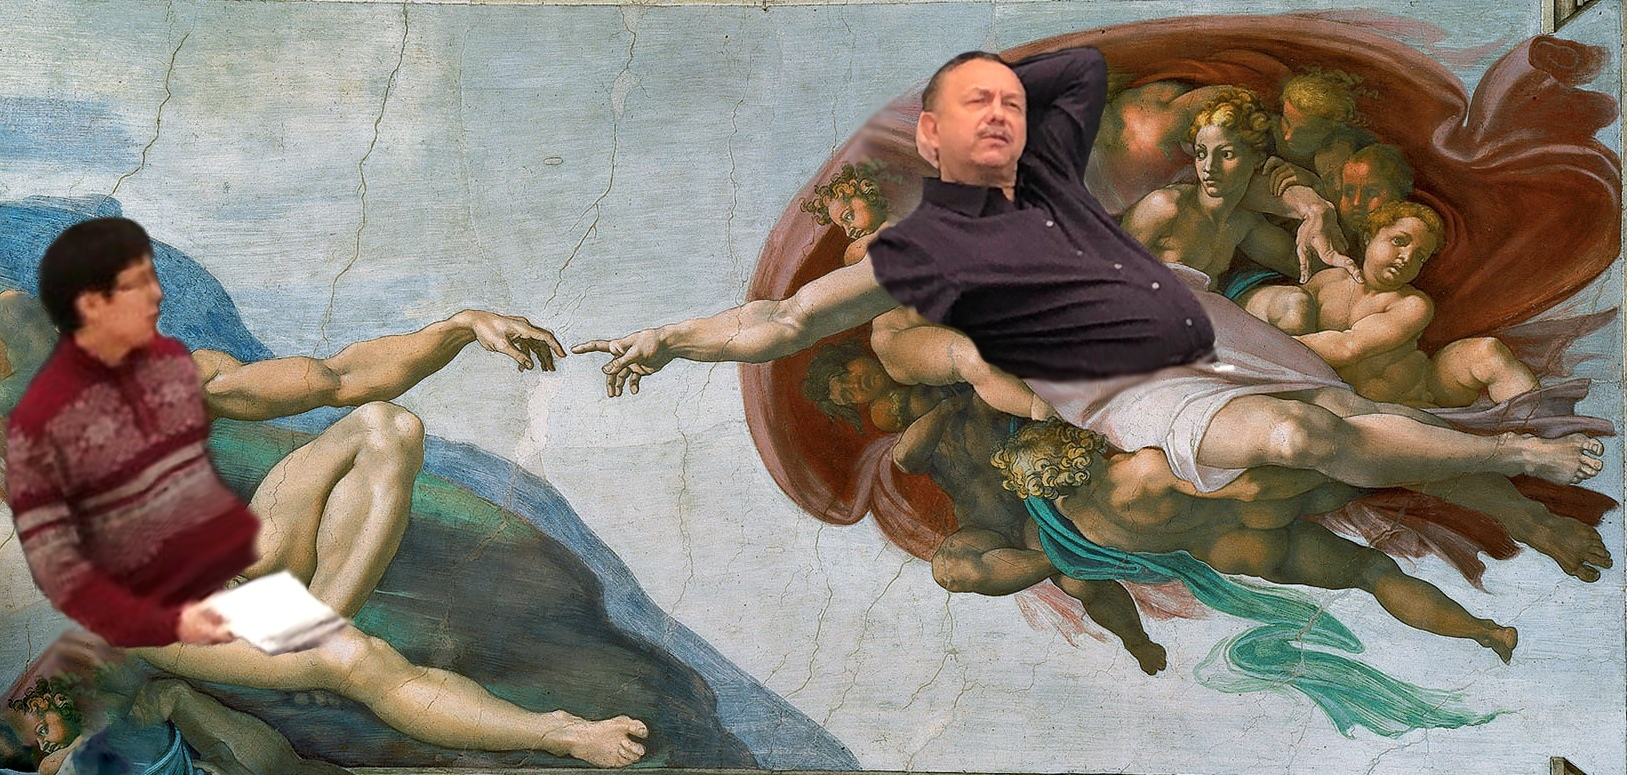
\includegraphics[scale=0.35]{images/palch.jpg}
\end{center}

\end{document}
